\documentclass[12pt]{article}

\usepackage[utf8]{inputenc}
\usepackage[T1]{fontenc}
\usepackage{amsmath,amssymb,amsthm}
\usepackage{graphicx}
\usepackage{booktabs}
\usepackage{multirow}
\usepackage[a4paper,margin=1in]{geometry}
\usepackage{setspace}
\usepackage[round,authoryear]{natbib}
\usepackage[hidelinks]{hyperref}

\doublespacing

\title{Measurement-Conditioned Framing Geometry: Contrastive NLI and Semantic Projection in Political News}
\author{Andrew Clair \\
Student Number: 22184813 \\
Supervisor: Henry Silke \\
Module: JM4018 - INDIVIDUAL JOURNALISM PROJECT 2025/6 SEM2}
\date{March 4, 2026}

\begin{document}

\maketitle

\begin{abstract}
Automated news aggregators frequently summarize political bias by projecting coverage onto an assumed one-dimensional spectrum using third-party publisher metadata, rather than measuring article text directly. We evaluate whether framing stance can be recovered as an endogenous low-dimensional geometry using frozen cross-encoder natural language inference (NLI) prompted with authored contrastive hypothesis pairs ($h_A, h_B$). Under an audited paired contrast operator ($s_A - s_B$) that removes response components shared between opposing hypotheses, article response covariance compresses onto a robust, primary stance axis ($\mathrm{PC1} \approx 42\% - 64\%$) that decisively clears 10,000-draw non-parametric permutation null gates ($p \le 0.0003$, detected rank strictly $k=1$) across both conflict and domestic policy domains (Israel--Palestine, Clean Ukraine $\mathrm{PC1} = 42.09\%, p = 0.0003$, US Immigration, Climate Politics, Abortion Rights). Synthetic factorial positive controls with known generating factors verify apparatus resolving power for higher-dimensional structure ($k=2$, $99.11\%$). Article stance coordinates reproduce across prospectively sampled text ($N=120$, $\mathrm{PC1} = 58.36\%$; cross-bank $r = 0.925$), non-overlapping disjoint probe partitions (mean $|r| \approx 0.76$ across 35 unique 4-vs-4 splits), and diverse transformer architectures (cross-model stance $r = 0.55 - 0.81$ across DeBERTa, BART, and RoBERTa).

We benchmark this relational NLI apparatus against a matched sentence-level semantic projection baseline (FrameAxis). Holding corpus and conceptual contrasts fixed, the two instruments produce weakly aligned dominant coordinates ($r \in [0.01, 0.19]$ standardized). Canonical correlation analysis reveals that this is not orthogonal noise: the instruments share a significant multivariate semantic subspace ($r_{\mathrm{canon,test}} = 0.364 \pm 0.080$, Monte Carlo permutation $p = 0.0010$) that generalizes out-of-sample under strictly fold-local repeated 5-fold cross-validation. Minimal compositional controls establish that NLI exhibits substantially greater compositional sensitivity on tested perturbations, achieving complete concordance and sign inversion on negation ($100\%$) and quantifiers ($100\%$, where dense projection collapses to cosine similarities of $0.73 - 0.99$), while remaining bounded on syntactic agent--patient reversal ($50\%$). Anisotropy-removal ablations demonstrate that dominant semantic projection variance is substantially driven by leading representation components ($73.7\% \to 34.5\%$ upon removing the top embedding PC), whereas NLI stance coordinates separate news outlets ($\eta^2 = 40.1\%, p = 0.005$) and survive collinear sentiment controls ($\eta^2 = 34.8\%, p = 0.022$). We conclude that low-dimensional framing structure is not unique to NLI, but the recovered dominant coordinate depends on the measurement operator: $\mathcal{G}_{\text{observed}} = f(C, H, O, M)$.
\end{abstract}

\newpage

\section*{Declaration}
I acknowledge the use of Gemini CLI, Codex CLI, and ChatGPT to generate the equation LaTeX, generation of repository code, as well as serving as a sounding board for the machine learning and mathematical operations as the system developed. I confirm that this is entirely my own work and that it has not been submitted for assessment as part of any other programme.

\vspace{1cm}
Signed: Andrew Clair \\
Date: January 12, 2026

\newpage

\section{Introduction and Literature Review}

This paper evaluates whether media framing and ideological stance can be recovered as an endogenous geometric manifold directly from article content, without relying on external publisher-level metadata. Contemporary news aggregators and media monitoring platforms (such as Ground News) frequently critique journalistic bias by mapping articles onto an assumed one-dimensional spectrum relative to an unmarked, objective ``center.'' In practice, however, such platforms classify coverage not by analyzing the text of individual articles, but by appending third-party ratings assigned to the publishing outlet as a whole. We critique this ``geometric fiction of objective neutrality'' \citep{bowkerstar1999,mouffe2000} and evaluate an alternative, content-grounded framework: probing news text with frozen cross-encoder natural language inference (NLI) prompted with authored contrastive hypothesis pairs ($(h_A, h_B)$).

Holding corpus and conceptual probes fixed, we benchmark this relational cross-attentive apparatus against a matched sentence-level semantic projection baseline \citep{kwak2021frameaxis}. Our empirical findings establish a clean scientific resolution:
\begin{equation*}
    \boxed{\text{Low-dimensionality is not unique to NLI}} \quad \text{and} \quad \boxed{\text{the recovered dominant coordinate depends on the measurement operator}}.
\end{equation*}
Under an audited paired contrast operator ($s_A - s_B$) that removes response components shared between opposing hypotheses, frozen NLI models consistently compress article response covariance onto a dominant rank-1 stance axis that decisively clears non-parametric permutation null gates ($p \le 0.0003$) across diverse conflict and domestic policy domains. This coordinate reproduces across prospectively sampled unseen text ($N=120, r = 0.925$), non-overlapping disjoint probe partitions (mean $|r| \approx 0.76$), and distinct model architectures ($r \in [0.55, 0.81]$). Furthermore, canonical correlation analysis demonstrates that NLI and semantic projection share a statistically significant multivariate semantic subspace ($r_{\mathrm{canon,test}} = 0.364$, Monte Carlo $p = 0.0010$) that generalizes out-of-sample under strictly fold-local cross-validation.

However, their dominant coordinates diverge sharply ($r \in [0.01, 0.19]$ standardized). Minimal compositional controls and anisotropy ablations identify the causal sources of this divergence: proposition-level NLI exhibits greater compositional sensitivity on tested perturbations (negation, quantifiers, causal direction) and captures systematic outlet differentiation ($\eta^2 = 40.1\%$) that survives sentiment controls ($\eta^2 = 34.8\%$), whereas naive semantic projection PC1 is substantially organized by the dominant representation geometry of the underlying embedding space ($73.7\% \to 34.5\%$ upon removing the top principal component). Consequently, the observed geometry of political discourse is fundamentally conditioned by the measurement operator:
\begin{equation}
    \mathcal{G}_{\text{observed}} = f(C,\; H,\; O,\; M),
\end{equation}
where corpus ($C$), hypothesis bank ($H$), measurement operator ($O$), and model ($M$) jointly determine which latent variation dominates.

\subsection{Ground News and Horizontal Metadata Expansion}

Ground News\footnote{Website link: \url{https://ground.news/}} is a prominent news aggregator designed to expose ``bias,'' which it operationalizes as a directional deviation from neutrality. The platform organizes reporting on political issues by placing articles along a left-center-right continuum relative to an assumed consensus baseline. While marketed as an instrument for critical media literacy and viewpoint pluralism, its classification architecture does not examine the semantic content of the individual articles it displays. Instead, it classifies articles horizontally: at ingestion, it queries third-party media monitoring organizations (principally AllSides, Ad Fontes Media, and Media Bias/Fact Check) to obtain an external, publisher-level rating, and appends this label to every article published by that outlet \citep{allsidesmethod,groundnewsrating}.

Formally, a horizontal metadata pipeline implements a mapping:
\begin{equation}
    H(a) = (a,\; m(p(a))),
\end{equation}
where $a$ is an article, $p(a)$ maps the article to its publishing organization, and $m(\cdot)$ retrieves static external metadata. The bias score is then computed as a projection over publisher metadata:
\begin{equation}
    b_{\text{hor}}(a) = \psi(m(p(a))),
\end{equation}
which is independent of the text content of $a$. If a prestigious legacy publication runs an adversarial opinion column, an investigative exposé, or an unedited wire dispatch, the horizontal pipeline assigns all three identical political coordinates based entirely on organizational identity.

This architectural dependency raises fundamental methodological concerns. Systems that claim to reveal bias often rely on antecedent classificatory frameworks that are external to the content they categorize, reinforcing conventional editorial boundaries and reifying an unmarked ``middle'' perspective as objective reality \citep{bowkerstar1999}. In contrast, an endogenous, content-level measurement extracts representations directly from the source text under declared analytical frames:
\begin{equation}
    x \mapsto \{z_h(x)\}_{h \in \mathcal{H}},
\end{equation}
deriving framing geometry from textual interaction rather than institutional proxy labels.

\subsection{Philosophical Foundations of Observer-Conditioned Semantics}

The critique of external neutrality connects directly to foundational debates in epistemology and the philosophy of science. Thomas Kuhn \citeyearpar{kuhn1962} argued that observation is inherently theory-laden: empirical data cannot be collected or interpreted outside of an interpretive paradigm. Nelson Goodman \citeyearpar{goodman1978} extended this insight into a formal theory of worldmaking, demonstrating that measurement systems do not merely describe preexisting structures, but actively construct the categories they map through their choice of frame, scale, and projection.

In this work, we operationalize Kuhn's insight computationally. Rather than invoking the observer as a vague metaphor, we formalize an interpretive \emph{paradigm} as an explicit four-tuple measurement system:
\begin{equation}
    P = (H,\; O,\; M,\; L),
\end{equation}
where:
\begin{itemize}
    \item $H$ denotes the conceptual distinctions the paradigm recognizes (the authored contrastive hypothesis bank or probe space);
    \item $O$ denotes the operational measurement rules (the mathematical operator, such as paired contrast $s_A - s_B$, single-side polarity $s_A$, or cosine projection $Z(P)$);
    \item $M$ denotes the representational machinery (the pre-trained transformer model, such as DeBERTa-v2, BART, or RoBERTa);
    \item $L$ denotes the analytical vocabulary and ontology through which observations are articulated.
\end{itemize}
The empirical discourse world presented by a fixed corpus $C$ under paradigm $P$ is the recovered geometry:
\begin{equation}
    \mathcal{G}_P(C) = f(C;\; P) = f(C,\; H,\; O,\; M).
\end{equation}
This formulation gives empirical research what classical philosophy of science lacked: an experimental apparatus capable of \emph{holding the empirical object ($C$) strictly fixed while systematically varying the interpretive paradigm ($P$)}. Two paradigms can interrogate the exact same articles and organize them into divergent relational spaces because they ask different questions, enforce different contrastive oppositions, and apply different measurement operators.

This experimental framework allows us to define a clear five-tier hierarchy of epistemological and ontological claims:
\begin{enumerate}
    \item \textbf{Tier 1 (Empirical)}: Changing the measurement operator or hypothesis bank substantially alters the recovered document geometry $\mathcal{G}(C)$.
    \item \textbf{Tier 2 (Epistemological)}: Observations of framing are theory-laden; framing measurements are conditioned by the representational apparatus through which the text is interrogated.
    \item \textbf{Tier 3 (Structural)}: Perspectivally robust invariants ($I(\mathcal{G}_{P_1}) \approx I(\mathcal{G}_{P_2})$) survive across changing paradigms---such as low effective dimensionality and extremal anchor ordering---even when local coordinates rotate: \emph{coordinates vary, but higher-order structure persists}.
    \item \textbf{Tier 4 (Ontological)}: Political framing is an \emph{ontologically relational property}. Rather than treating bias as an intrinsic substance or text-internal scalar attribute $B(x) \in [-1, 1]$, framing stance exists as a relation $B(x; P) = R(x, P)$ instantiated between a text and an interpretive scheme. Just as velocity is relational ($v(A \mid B)$) rather than an intrinsic property like rest mass ($m(A)$), an article's political stance is fundamentally relational. A text possesses intrinsic syntactic and lexical tokens (e.g., casualty numbers or event nouns), but its framing stance is an emergent relational property under an interrogated paradigm.
    \item \textbf{Tier 5 (Metaphysical Boundary)}: We falsify the empirical existence of any single, privileged, observer-independent paradigm $P^*$ within the tested family; we explicitly do not claim to establish total metaphysical relativism or deny the existence of an external reality.
\end{enumerate}

In computational linguistics, this insight connects with \emph{perspectivist NLP} \citep{frenda2024,xujurgens2026}. Rather than forcing divergent annotator judgments into a single aggregated consensus label, perspectivist approaches treat interpretive variation as a primary information signal. Empirical studies of natural language inference demonstrate that even under standardized annotation guidelines, human semantic judgments on complex propositions exhibit persistent, structured divergence \citep{pavlick2019}. Attempting to eliminate this divergence by post-hoc averaging or increasingly coercive annotation manuals often merely perfumes the consensus metrics \citep{aroyo2015}, suppressing the legitimate interpretive ambiguities that constitute ideological discourse. Natural language inference provides a rigorous mechanism for operationalizing perspectival analysis without supervised fine-tuning on political labels, evaluating whether proposition $h_A$ logically follows from the text more strongly than $h_B$.

\subsection{Pluralism, Civility, and Democratic Agonism}

The assumption that media bias can be neutralized by locating an arithmetic center reflects a specific, and contested, political philosophy. In political theory, Chantal Mouffe \citeyearpar{mouffe2000} critiques consensus-driven models of liberal democracy, arguing that genuine political conflict cannot be transformed into technical consensus without disenfranchising legitimate dissent. Real-world politics is irreducibly \emph{agonistic}: it consists of conflicting, legitimate interpretations of justice, sovereignty, and rights that cannot be dissolved into an unproblematic middle ground.

Similarly, Alison Reiheld \citeyearpar{reiheld2013}, drawing on Isaiah Berlin's \citeyearpar{berlin1998} value pluralism, demonstrates that projects enforcing ``exceptionless civility'' frequently prioritize institutional social management over democratic pluralism. By sanitizing rhetorical friction and treating disagreement as a pathological deviation from consensus, middle-ground aggregators risk manufacturing a depoliticized center that silences structural critique. Journalistic reporting on violent conflict or polarized policy debates does not deviate from a natural baseline; it navigates conflicting worldviews whose tensions require explicit, transparent measurement containers rather than statistical erasure \citep{swanstromweissmann2005}.

\subsection{Representation, Projection, and the Measurement Operator}

When analyzing complex semantic representations, high-dimensional spaces must inevitably be projected onto lower-dimensional coordinates for human interpretation. News aggregators heuristically compress coverage into a single left-right axis. The fundamental error occurs when this single coordinate is treated as an objective, observer-independent ground truth. As Ludwig Wittgenstein observed, the perspective from which a system is described cannot be placed inside the description itself: ``the subject does not belong to the world but it is a limit of the world'' \citep{wittgenstein1922}. Every coordinate system is an artifact of its projection apparatus.

In computational social science, this raises a central methodological challenge: how does the mathematical measurement operator condition the recovered geometry? The dominant paradigm in framing analysis projects text embeddings onto semantic axes defined by antonym pole vectors \citep{kwak2021frameaxis}. However, dense embedding spaces are notoriously susceptible to representation anisotropy, organizing token representations into narrow cones governed by lexical frequency and sequence length \citep{gabaix1999,mu2018allbutthetop}. Furthermore, independent vector encoders lack joint cross-attention, causing meaning-reversing compositional operations (such as negation or quantifier inversion) to collapse into near-identical cosine proximities \citep{ettinger2020}.

Crucially, this framework allows us to turn Kuhn's concept of \emph{incommensurability} into a measurable empirical hypothesis. Rather than a metaphysical slogan that frameworks cannot communicate, incommensurability can be operationalized by testing whether there exists a low-distortion transformation $T_{A \to B}$ such that $T_{A \to B}(\mathcal{G}_A) \approx \mathcal{G}_B$. If no linear, affine, or rigid transformation can simultaneously preserve article orderings, relational distances, and topological neighborhoods, the paradigms exhibit measurable incommensurability. Furthermore, by evaluating local $k$-nearest-neighbor Jaccard overlap $J_k(x; P_A, P_B)$, we can empirically test Kuhnian ``world change'': whether shifting the conceptual paradigm fundamentally alters which documents resemble which. Finally, by defining anomaly scores $A_P(x)$ as residual variance off the dominant paradigm manifold, we can interrogate whether anomalies are text-intrinsic properties or emergent relational collisions between text and paradigm.

This paper interrogates the empirical consequences of that architectural choice across corpora, conceptual frames, and operators. Specifically, we investigate:
\begin{enumerate}
    \item Whether authored contrastive hypotheses elicit reproducible low-dimensional framing structure from frozen NLI models across prospective news text, disjoint probe splits, and diverse policy domains;
    \item Whether apparatus resolving power can distinguish genuine multi-dimensional factor structure ($k=2$) from rank-1 collapse under synthetic factorial positive controls with known generating factors;
    \item Whether the recovered stance ordering aligns with or diverges from matched semantic-axis projections, and whether canonical correlation analysis reveals a shared underlying semantic subspace;
    \item What mechanistic factors (compositional sensitivity versus representation anisotropy) explain the organization of their respective dominant coordinates;
    \item Whether varying the conceptual and operator paradigm operationalizes a measurable form of Kuhnian incommensurability, relational neighborhood shift (``world change''), and anomaly relativity, while preserving higher-order structural invariants.
\end{enumerate}
In the following methodology, we formalize the measurement apparatus, the corpus construction protocols, the non-parametric permutation gates, and the diagnostic baseline comparisons.

\section{Methodology}

This section details the empirical pipeline used to measure framing geometry from text without external supervision. The methodology is organized around ten core components: (1)~authored contrastive hypothesis pairs and the audited paired NLI operator; (2)~corpus construction, prospective sampling protocols, and syndication sensitivity; (3)~non-parametric dimensionality gating and disjoint-bank stability; (4)~cross-model and cross-topic replication; (5)~the matched sentence-level semantic projection baseline; (6)~minimal compositional controls; (7)~standardized PCA and representation anisotropy ablations; (8)~canonical correlation analysis with strictly fold-local cross-validation; (9)~publisher differentiation ANOVA and sentiment nuisance controls; and (10)~methodological scope and developmental audit of excluded machinery.

\subsection{Contrastive Hypothesis Measurement and the Audited Paired Operator}
\label{sec:meth_paired_operator}

The primary measurement apparatus evaluates an article $x \in \mathcal{X}$ against a bank of authored contrastive hypothesis pairs, $\mathcal{H} = \{(h_A^{(k)}, h_B^{(k)})\}_{k=1}^K$ ($K=8$), using a frozen natural language inference (NLI) cross-encoder. In our primary implementation, we employ \texttt{DeBERTa-v2-xlarge-mnli} \citep{he2021deberta}, which processes document $x$ and hypothesis $h$ simultaneously through 24 layers of disentangled self-attention.

For each forward pass, the model outputs three unnormalized logits $(z_E, z_N, z_C) \in \mathbb{R}^3$, corresponding to entailment, neutral, and contradiction. Softmax normalization yields probability scores:
\begin{equation}
    P(c \mid x, h) = \frac{\exp(z_c)}{\sum_{c' \in \{E, N, C\}} \exp(z_{c'})}, \quad c \in \{E, N, C\}.
\end{equation}
We define the directional polarity score of document $x$ with respect to hypothesis $h$ as the entailment-minus-contradiction margin:
\begin{equation}
    s(x, h) = P(\text{entailment} \mid x, h) - P(\text{contradiction} \mid x, h) \in [-1, 1].
\end{equation}

When evaluating opposing framing propositions $(h_A^{(k)}, h_B^{(k)})$, two distinct measurement operators can be constructed:
\begin{enumerate}
    \item \textbf{Single-Side Margin ($s_A$)}: Evaluates document polarity exclusively against the primary hypothesis pole:
    \begin{equation}
        s_A^{(k)}(x) = s(x, h_A^{(k)}).
    \end{equation}
    \item \textbf{Audited Paired Contrast Operator ($s_A - s_B$)}: Evaluates the differential displacement between opposing propositions:
    \begin{equation}
        M_k(x) = s_A^{(k)}(x) - s_B^{(k)}(x) = \left[P(E \mid x, h_A^{(k)}) - P(C \mid x, h_A^{(k)})\right] - \left[P(E \mid x, h_B^{(k)}) - P(C \mid x, h_B^{(k)})\right].
    \end{equation}
\end{enumerate}
The paired contrast operator ($s_A - s_B$) removes response components shared between the opposing hypotheses ($s_A + s_B$). Whether those shared components reflect general topical salience, shared vocabulary compatibility, or baseline probability mass, subtracting $s_B$ from $s_A$ ensures that the resulting score isolates differential stance rather than common-mode activation. For an $N$-document corpus, evaluating $K$ contrastive pairs yields the audited response matrix $M \in \mathbb{R}^{N \times K}$.

\subsection{Corpora Construction, Prospective Protocol, and Syndication Sensitivity}
\label{sec:meth_corpora}

The empirical evaluation encompasses six distinct corpus configurations across foreign conflict, domestic policy, and synthetic factorial designs:
\begin{enumerate}
    \item \textbf{Prospective Confirmatory Corpus ($N=120$, 70 publishers)}: To prevent post-hoc sample optimization, 120 news articles on the Israel--Palestine conflict published between August and September 2024 were sampled prospectively under a frozen exact-fingerprint exclusion registry (registry hash \texttt{03be740c}). Every prospective candidate URL, title string, and SHA-256 text hash was filtered against a quarantine database of 1,290 historical project texts, ensuring zero collisions. The resulting corpus represents 70 unique publishing outlets.
    \item \textbf{Syndication Sensitivity Subset ($N=83$)}: To assess wire syndication artifacts, all 120 prospective articles were subjected to a pairwise 5-token shingle Jaccard similarity audit. While exact deduplication succeeded, 37 articles exhibited high content overlap ($\text{Jaccard} \ge 0.50$) due to syndicated wire republication across different regional outlets (e.g., identical Reuters or AP copy republished under local mastheads). The clean non-syndicated subset ($N=83$) strictly excludes all syndicated duplicates.
    \item \textbf{Clean Deduplicated Ukraine Corpus ($N=60$, 54 publishers)}: Foreign conflict reporting on the Russia--Ukraine war collected across 54 independent publishers, filtered to ensure all pairwise 5-token Jaccard similarities remain strictly $\le 0.35$, resolving syndication clustering present in early exploratory pilots.
    \item \textbf{Multi-Domain Domestic Policy Corpora ($N=60$ each)}: Three independent US policy domains evaluated under matched contrastive hypothesis banks: US Immigration \& Border Policy (51 publishers), Climate Politics (51 publishers), and Abortion Rights (55 publishers).
    \item \textbf{Controlled Balanced Corpus ($N=60$, 12 publishers $\times$ 5 articles)}: A balanced sample of 12 distinct international and domestic news outlets with exactly 5 articles per outlet, constructed specifically to evaluate publisher stance differentiation.
    \item \textbf{Synthetic Factorial Positive Control ($N=60$)}: A controlled $2 \times 2$ factorial corpus crossing two orthogonal generating factors: \emph{Security Threat} (high vs.\ low) $\times$ \emph{Civilian Harm} (high vs.\ low), with 15 balanced articles per quadrant, generated with known generating factors to verify apparatus resolving power for higher-dimensional structure ($k=2$).
\end{enumerate}

\subsection{Non-Parametric Dimensionality Gating and Disjoint-Bank Stability}
\label{sec:meth_dimensionality}

To determine whether the $N \times K$ article response matrix $M$ reflects low-dimensional framing structure or high-dimensional noise, we decompose the column-centered matrix $M - \mathbf{1}\mu^\top$ via Singular Value Decomposition (SVD):
\begin{equation}
    M - \mathbf{1}\mu^\top = U \Sigma V^\top.
\end{equation}
The eigenvalues $\lambda_j = \frac{\sigma_j^2}{N-1}$ quantify variance along principal axis $j$. The explained variance ratio ($\mathrm{EVR}$) and participation ratio ($\mathrm{PR}$) are:
\begin{equation}
    \mathrm{EVR}_j = \frac{\lambda_j}{\sum_{i=1}^K \lambda_i}, \qquad \mathrm{PR} = \frac{\left(\sum_{i=1}^K \lambda_i\right)^2}{\sum_{i=1}^K \lambda_i^2}.
\end{equation}

To establish the statistical significance of each component without making distributional assumptions, we evaluate eigenvalues against non-parametric permutation null models:
\begin{itemize}
    \item \textbf{Column Permutation Null (10,000 draws)}: For each draw $b \in \{1, \ldots, 10000\}$, the entries of each column of $M$ are permuted independently. This preserves the exact marginal distribution of each probe pair while destroying inter-axis covariance.
    \item \textbf{Publisher-Block Permutation Null (10,000 draws)}: On corpora with publisher clustering, whole publisher blocks are permuted, preserving within-outlet correlation.
\end{itemize}
For each principal component $j$, the empirical null distribution yields a 95th-percentile threshold ($q_{95}$). We compute plus-one Monte Carlo $p$-values:
\begin{equation}
    p_j = \frac{1 + \sum_{b=1}^{B} \mathbb{I}\left(\lambda_{j,\text{null}}^{(b)} \ge \lambda_{j,\text{obs}}\right)}{1 + B}.
\end{equation}
The detected dimensionality (effective rank $k$) is defined strictly as the number of consecutive components clearing the permutation gate ($p_j \le 0.05$ and $\lambda_{j,\text{obs}} > q_{95}$).

To ensure that recovered stance coordinates reflect a distributed property of the discourse rather than an artifact of a single dominant prompt pair, we execute a \textbf{Complementary Disjoint-Bank Stability Analysis}. We evaluate all $\binom{8}{4}/2 = 35$ unique complementary 4-vs-4 partitions ($S \subset \{1, \ldots, 8\}, |S|=4$, with $S \cap S^c = \emptyset$). For each split, we fit PCA independently on sub-matrix $M_S$ and sub-matrix $M_{S^c}$, project documents onto their respective first principal components ($\mathrm{PC1}_S$ and $\mathrm{PC1}_{S^c}$), and record the cross-partition Pearson correlation $r(S, S^c)$. Because the two sub-banks share zero variables, this eliminates the part-whole correlation inflation inherent in leave-one-axis-out diagnostics.

\subsection{Cross-Model and Cross-Topic Replication}
\label{sec:meth_cross_model}

To evaluate whether the observed rank-1 compression reflects the semantic relation between text and hypotheses or an architecture-specific artifact of DeBERTa's decoupled embeddings, we benchmark three distinct transformer cross-encoders on the balanced $N=60$ corpus:
\begin{itemize}
    \item \texttt{microsoft/deberta-v2-xlarge-mnli} (900M parameters, disentangled attention);
    \item \texttt{facebook/bart-large-mnli} (406M parameters, sequence-to-sequence encoder-decoder);
    \item \texttt{roberta-large-mnli} (355M parameters, bidirectional transformer encoder).
\end{itemize}
For each model, we extract the audited paired matrix $M$, evaluate 10,000-draw permutation null gates, and compute pairwise article stance correlations ($r, \rho$) and principal subspace angles between models.

To evaluate cross-topic generalization, the identical paired operator and permutation gating battery are deployed across US Immigration, Climate Politics, Abortion Rights, and Clean Ukraine. Additionally, exploratory conceptual-lens tests ($Q_2$ Humanitarian Rights and $Q_3$ Realpolitik Statecraft) authored in the same AI-assisted development session are evaluated as secondary vocabulary sensitivity checks, with confirmatory claims restricted to the primary $Q_0$ and $Q_1$ banks.

\subsection{Matched FrameAxis-Style Semantic Projection Baseline}
\label{sec:meth_frameaxis}

To test whether proposition-level NLI is redundant with existing vector-space methods, we construct a matched \textbf{FrameAxis-style sentence-level semantic projection baseline} \citep{kwak2021frameaxis}. Whereas original FrameAxis aggregated word- and token-level embeddings, our baseline directly embeds whole propositions and whole documents using modern sentence encoders, providing a strictly stronger comparator.

Let $e(\cdot) \in \mathbb{S}^{d-1}$ denote an $L_2$-normalized embedding encoder ($\|e\|_2 = 1$). For document $x$ and contrastive hypothesis pair $k$ with poles $(h_A^{(k)}, h_B^{(k)})$, we compute two projection operators:
\begin{enumerate}
    \item \textbf{Primary FrameAxis Cosine Difference ($F_k$)}:
    \begin{equation}
        F_k(x) = \cos(e(x), e(h_A^{(k)})) - \cos(e(x), e(h_B^{(k)})) = \langle e(x),\, e(h_A^{(k)}) - e(h_B^{(k)}) \rangle.
    \end{equation}
    \item \textbf{Normalized Vector Projection ($P_k$)}: Let $v_k = e(h_A^{(k)}) - e(h_B^{(k)})$ define the semantic axis. The normalized projection onto $v_k$ is:
    \begin{equation}
        P_k(x) = \frac{\langle e(x), v_k \rangle}{\|e(x)\|_2 \|v_k\|_2} = \frac{F_k(x)}{\|v_k\|_2}.
    \end{equation}
\end{enumerate}
Because $\|v_k\|_2$ is a strictly positive constant for each axis $k$, $P_k(x)$ is an exact positive column rescaling of $F_k(x)$. Under column-standardized PCA ($Z_{ik} = \frac{M_{ik} - \mu_k}{\sigma_k}$), $Z(P)$ and $Z(F)$ are mathematically identical:
\begin{equation}
    Z_{ik}(P) \equiv Z_{ik}(F).
\end{equation}
We evaluate FrameAxis projections under both DeBERTa-v2-xlarge sequence embeddings and a dedicated sentence encoder (\texttt{sentence-transformers/all-MiniLM-L6-v2}).

\subsection{Minimal Compositional Controls Diagnostic Benchmark}
\label{sec:meth_compositional}

To diagnose why joint cross-encoding and vector-space projection diverge, we construct a diagnostic benchmark of 16 minimal sentence pairs across four perturbation categories ($N=4$ pairs per category):
\begin{enumerate}
    \item \textbf{Polarity Negation}: Direct negation of the main verb or predicate (e.g., ``Forces ceased fire'' $\leftrightarrow$ ``Forces did not cease fire'');
    \item \textbf{Quantifier Inversion}: Inversion of universal/existential quantifiers (e.g., ``All civilian corridors were opened'' $\leftrightarrow$ ``No civilian corridors were opened'');
    \item \textbf{Causal Direction Reversal}: Inversion of antecedent and consequence (e.g., ``Airstrikes caused the collapse of talks'' $\leftrightarrow$ ``The collapse of talks caused airstrikes'');
    \item \textbf{Agent--Patient Role Reversal}: Syntactic subject-object swapping (e.g., ``Militants ambushed the patrol'' $\leftrightarrow$ ``The patrol ambushed militants'').
\end{enumerate}
For each minimal pair $(x, x')$ and relevant contrastive pair $k$, we specify the expected direction of stance change ($\operatorname{expected\_sign} \in \{+1, -1\}$) and evaluate two metrics:
\begin{itemize}
    \item \textbf{Directional Concordance}: Proportion of pairs where the observed shift matches the expected sign:
    \begin{equation}
        \operatorname{sgn}(M_k(x) - M_k(x')) = \operatorname{expected\_sign}.
    \end{equation}
    \item \textbf{Zero-Crossing Sign Inversion}: Proportion of pairs where the perturbation flips the sign of the stance score:
    \begin{equation}
        M_k(x) \cdot M_k(x') < 0.
    \end{equation}
\end{itemize}

\subsection{Standardized PCA and Representation Anisotropy Ablations}
\label{sec:meth_anisotropy}

Because raw covariance PCA is sensitive to scale heterogeneity across axes, we report both raw covariance PCA ($M_{\text{raw}}$) and column-standardized correlation PCA ($Z(M)$) across all corpora.

To examine whether dense FrameAxis PC1 reflects genuine political discourse or representation geometry, we compute correlation diagnostics between document projection scores and known signatures of embedding anisotropy:
\begin{itemize}
    \item Correlation with raw hidden-state sequence embedding $L_2$ norm ($\|e(x)\|_2$);
    \item Correlation with cosine similarity to the global mean embedding ($\cos(e(x), \bar{e})$).
\end{itemize}
We then apply anisotropy-removal transformations to embedding space prior to FrameAxis projection \citep{mu2018allbutthetop}:
\begin{enumerate}
    \item \textbf{Mean Centering}: Centering representations by subtracting the global mean: $e \to e - \bar{e}$.
    \item \textbf{Top-1 PC Removal (Primary Confirmatory Diagnostic)}: Projecting out the dominant principal component of the embedding space:
    \begin{equation}
        e \to e - \langle e, u_1 \rangle u_1.
    \end{equation}
    \item \textbf{Top-2 PC Removal (Exploratory Follow-Up)}: Projecting out the top two principal components:
    \begin{equation}
        e \to e - \sum_{j=1}^2 \langle e, u_j \rangle u_j.
    \end{equation}
\end{enumerate}

\subsection{Canonical Correlation Analysis with Strict Fold-Local Cross-Validation}
\label{sec:meth_cca}

To test whether the 8D NLI response matrix $X \in \mathbb{R}^{N \times 8}$ and the 8D FrameAxis projection matrix $Y \in \mathbb{R}^{N \times 8}$ share a multivariate semantic subspace despite divergent dominant axes, we evaluate Canonical Correlation Analysis (CCA). CCA finds linear combinations $w_x, w_y \in \mathbb{R}^8$ that maximize the correlation between canonical variates:
\begin{equation}
    r_{\mathrm{canon}} = \max_{w_x, w_y} \operatorname{corr}(X w_x,\, Y w_y).
\end{equation}

Because in-sample CCA optimizes linear weights and can exhibit upward sample bias, we evaluate statistical validity using two protocols with train-fitted preprocessing:
\begin{enumerate}
    \item \textbf{Monte Carlo Permutation Null (1,000 draws)}: Permuting document rows of $Y$ relative to $X$, generating an empirical null distribution for leading canonical correlation.
    \item \textbf{Strictly Fold-Local Repeated 5-Fold Cross-Validation}: To eliminate preprocessing leakage, column standardizers ($\mu_{\text{train}}, \sigma_{\text{train}}$) and canonical projection weights $(W_X, W_Y)$ are fit exclusively on training observations ($4/5$ split). Held-out test folds ($1/5$ split) are transformed out-of-sample and evaluated for test correlation. We execute 50 random 5-fold CV repeats (250 distinct test folds), reporting pooled out-of-sample correlation ($r_{\mathrm{canon,test}}$) and mean within-fold test correlation.
\end{enumerate}

\subsection{Publisher Differentiation ANOVA and Sentiment Nuisance Controls}
\label{sec:meth_anova}

To establish whether recovered coordinates carry external journalistic signal, we evaluate one-way Analysis of Variance (ANOVA) across publishers on the balanced Controlled $N=60$ corpus (12 publishers $\times$ 5 articles):
\begin{equation}
    F = \frac{\mathrm{MS}_{\text{between}}}{\mathrm{MS}_{\text{within}}}, \qquad \eta^2 = \frac{\mathrm{SS}_{\text{between}}}{\mathrm{SS}_{\text{total}}}.
\end{equation}
Non-parametric Kruskal--Wallis $H$-tests are evaluated in parallel.

Because political stance correlates with emotional valence, we implement a \textbf{Collinear Sentiment Nuisance Control}. We extract VADER sentiment scores (positive, negative, and compound valence) for each article. Because compound valence is mathematically derived from positive and negative valence, multivariate sentiment regression ($PC1_i = \beta_0 + \beta^\top \mathbf{s}_i + \epsilon_i$) serves as a nuisance sensitivity control rather than an orthogonal decomposition of affect. We then evaluate whether residual publisher separation on $\epsilon_i$ remains statistically significant. We emphasize that publisher separation demonstrates systematic outlet differentiation (reflecting editorial stance, topic selection, and sourcing) rather than external ideological ground truth.

\subsection{Methodological Scope and Developmental Audit of Excluded Machinery}
\label{sec:meth_excluded}

A key methodological contribution of this study is the adversarial audit that identified and quarantined uncalibrated constructs developed during early exploratory iterations:
\begin{itemize}
    \item \textbf{Random Kitchen Sinks (RKS)}: Explored as an explicit kernel approximation in earlier drafts; ablation testing demonstrated that raw representations perform equivalently or superiorly to RKS expansions. Kernels function as similarity metrics, not independent epistemological observers.
    \item \textbf{Dirichlet Simplex Annealing}: Originally motivated by Homotopy Type Theory (HoTT) analogies of path obstruction; audit revealed that legacy tests treated non-independent article dyads as independent samples. Dirichlet cooling represents a finite-dimensional optimization over mixture weights, not a topological invariant.
    \item \textbf{Sheaf Cocycle Holonomy}: Quarantined after algebraic audit revealed that legacy code inverted composition order ($R_{jk}R_{ij}$ vs.\ $R_{ij}R_{jk}$) and lacked an empirical null distribution.
    \item \textbf{Continuous Third-Party Benchmarks (MBFC)}: Evaluated on small publisher samples ($N=11, N=16$); demonstrated acute sensitivity to single publisher exclusions (e.g., Press TV), leading to its demotion from primary validation to an issue-specific divergence flagger.
\end{itemize}
By pruning this uncalibrated machinery, the resulting empirical apparatus rests strictly on reproducible, non-parametric statistical tests and controlled experimental comparisons.

\subsection{Adversarial Falsification Protocol and Empirical Claim Gates}
\label{sec:meth_claim_gates}

To guard against confirmation bias and prevent post-hoc reinterpretation of philosophical constructs, we subject the Kuhnian interpretive framework to an explicit adversarial follow-up with pre-specified falsification gates (\path{scripts/exp_adversarial_kuhnian_battery.py}, \path{paper/adversarial_kuhnian_audit_results.json}). Rather than seeking unconstrained defense of ``incommensurability'' or ``world change,'' this protocol constructs the strongest empirical alternatives to explain the findings away, assigning each theoretical claim an explicit, quantitative disqualification condition.

\subsubsection{The Six-Agent Adversarial Protocol}
The campaign organizes six interlocking methodological audits:
\begin{enumerate}
    \item \textbf{Agent A (Provenance and Fail-Closed Hash Manifest)}: Computes SHA-256 hashes for all corpora, hypothesis banks, scripts, and model checkpoints, generating an immutable registry (\path{paper/experiment_manifest.json}). It strictly audits margin formulations, ensuring paired contrast ($s_A - s_B$) and single-side margins ($s_A$) are never conflated, and verifies zero exact collisions under the frozen registry across the audited corpora, with known post-hoc syndication overlap sensitivity.
    \item \textbf{Agent B (Within-Paradigm Reliability Noise Floor)}: Before evaluating cross-paradigm divergence, Agent~B establishes how much the \emph{same paradigm diverges from itself} under measurement resampling. For both $P_{\mathrm{NLI}}$ ($Q_0$) and $P_{\mathrm{FA}}$, we execute 1,000 bootstrap draws ($N=120$ with replacement), including out-of-bag evaluation, and 1,000 independent 50/50 split-half draws ($N_1=N_2=60$). Each scaler and PCA is fitted on its own resample; full-sample concordance and held-out reconstruction are reported separately. We compute within-paradigm stability for PC1 correlation ($r_{\text{same}}$), 2D Procrustes disparity ($\mathcal{D}_{\text{same}}$), neighborhood overlap ($J_{k,\text{same}}$), and anomaly scores ($r(A_{\text{same}}^{(1)}, A_{\text{same}}^{(2)})$). For any cross-paradigm comparison, we evaluate the \emph{excess disparity}:
    \begin{equation}
        \Delta \mathcal{D}(P_A, P_B) = \mathcal{D}(P_A, P_B) - \frac{1}{2}\left[\mathcal{D}_{\text{same}}(P_A) + \mathcal{D}_{\text{same}}(P_B)\right].
    \end{equation}
    \emph{Kill Condition}: If cross-paradigm divergence is within the resampling noise floor ($\Delta \mathcal{D} \le 0$ or $J_{\text{cross}} \ge J_{\text{same}}$), the divergence claim is falsified as measurement instability.
    \item \textbf{Agent C (14-Level Translation Ladder)}: Tests whether divergent paradigm geometries can be mapped into one another by systematic functional transformations. We construct an ordered hierarchy of 14 models spanning increasing capacity ($T_0$ Sign Flip, $T_1$ Orthogonal Procrustes, $T_2$ Similarity Transform, $T_3$ Anisotropic Scaling, $T_4$ Affine OLS, $T_5$ RidgeCV, $T_6$ PLS-2, $T_7$ CCA, $T_8$ Degree-2 Poly-Ridge, $T_9$ Kernel Ridge RBF, $T_{10}$ Shallow MLP, $T_{11}$ Optimal Transport Barycentric Map, $T_{12}$ Piecewise Linear Charts, and $T_{13}$ $k$-NN Regressor). All models use five outer held-out folds with train-fitted preprocessing. Hyperparameters are fixed except where an estimator explicitly uses inner training-fold selection; the entire ladder is therefore not uniformly nested CV. Complexity is the ordered rung index $c$, with $c^\star(\tau)=\min\{c:Q(c)\geq\tau\}$, $Q(c)=R^2_{\mathrm{test}}$, and $\tau\in\{0.10,0.30,0.50\}$. An unattained threshold is reported explicitly.
    \emph{Kill Condition}: If low-capacity mappings ($T_0$--$T_5$) predict held-out cross-paradigm geometry with high fidelity ($R^2_{\text{test}} > 0.70$ and $J_{10,\text{test}} > 0.40$), incommensurability is falsified as trivial linear coordinate rotation.
    \item \textbf{Agent D (Calibrated Neighborhood Curves and Whitening Sensitivity)}: Sweeps $k \in \{3, 5, 10, 15, 20, 30, 50\}$ against eight reference null models (hypergeometric random subsets, permutation null, same-paradigm bootstrap, paraphrase control, Gaussian embeddings, anisotropic spectrum-matched synthetic null, TF-IDF lexical overlap, and publisher overlap). To test whether neighborhood dissolution is an artifact of transformer representation anisotropy, both response matrices are transformed via Zero-phase Component Analysis (ZCA) whitening ($W = U \Lambda^{-1/2} U^\top$) prior to nearest-neighbor graph construction.
    \emph{Kill Condition}: If cross-paradigm neighborhood dissolution vanishes under ZCA whitening, the finding is downgraded to a representation-geometry artifact.
    \item \textbf{Agent E (Multi-Definition Anomaly Relativity Battery)}: Formalizes six distinct mathematical anomaly definitions: $A_1$ (Rank-1 PCA subspace residual), $A_2$ (Rank-2 PCA residual), $A_3$ (Local Outlier Factor), $A_4$ (Mahalanobis distance), $A_5$ (Isolation Forest score), and $A_6$ (Minimum Covariance Determinant robust distance). It evaluates the full $6 \times 6$ anomaly transfer matrix $R_{ij} = r(A_{P_i}, A_{P_j})$.
    \emph{Kill Condition}: If cross-paradigm anomaly correlation is within resampling noise ($r_{\text{cross}} \approx r_{\text{same}}$) or if same-paradigm reliability is near zero ($r_{\text{same}} \approx 0$), anomaly relativity is falsified as estimation noise.
    \item \textbf{Agent F: AI-Authored Disciplinary-Bank Controls}: Uses AI-authored controls representing five disciplinary vocabularies under a frozen protocol (\path{config/prompt_banks/adversarial_and_disciplinary_banks.json}): International Humanitarian Law ($H_{\text{IHL}}$), Strategic Security ($H_{\text{Sec}}$), Peace \& Conflict Studies ($H_{\text{Peace}}$), Realist International Relations ($H_{\text{Real}}$), and Media Framing Analysis ($H_{\text{Journ}}$). True independent, blind human disciplinary authoring remains undone; these controls cannot establish human perspectival invariance.
\end{enumerate}

\subsubsection{Three Extreme Reductio Stress Tests}
To subject the framework to destructive limits, we formulate three extreme stress tests:
\begin{enumerate}
    \item \textbf{Reductio 1 (Absurd Structurally-Matched Paradigms)}: Evaluates four domain-null prompt banks matched in sentence length, syntax, and polarity contrast: Meteorology, Culinary Arts, Botanical Taxonomy, and Sports Tactics. For these four banks and $Q_0$, 10,000 independent column permutations calibrate eigenvalue thresholds and participation ratios. Publisher ANOVA is reported with raw, Benjamini--Hochberg FDR, and Bonferroni $p$-values across the four absurd-bank tests.
    \item \textbf{Reductio 2 (Maximally Distant Political Ontologies)}: Evaluates five radically disparate ontologies of the same conflict: Legal Culpability, Operational Efficacy, Humanitarian Welfare, Macroeconomic Cost, and Religious Obligation. We fit both standardizers and CCA exclusively on each training fold and measure canonical correlation on five held-out folds. A 1,000-draw row-permutation test refits the complete procedure; $p=(1+b)/(1001)$ is a Monte Carlo permutation value, not exhaustive enumeration. Empirical fold and null intervals are distinguished from population confidence intervals.
    \item \textbf{Reductio 3 (Adversarial Geometry Manufacturing \& Observer Pushback)}: Tests whether an observer can deliberately force arbitrary target geometries (e.g., inverted PC1 ordering, orthogonal distractors) onto corpus $C$, searching a finite registry of semantically constrained hypothesis contrast pairs for three explicit targets: inverted publisher ordering, forced publisher clustering, and an orthogonal distractor projection. The objective is $H^\star=\arg\min_H d(\mathcal{G}_H(C),G^\star)$. Failure within this candidate set does not establish impossibility over all plausible hypotheses.
\end{enumerate}

\begin{table}[ht]
\centering
\small
\caption{Pre-Specified Falsification Gates for Adversarial Follow-Up. These gates bound the empirical interpretation; they are not a retrospective preregistration claim.}
\label{tab:claim_gates}
\resizebox{\textwidth}{!}{%
\begin{tabular}{p{3.4cm}p{4.5cm}p{5.2cm}c}
\toprule
\textbf{Theoretical Claim} & \textbf{Operational Requirement} & \textbf{Disqualification / Kill Condition} & \textbf{Audit Status} \\
\midrule
\textbf{Measurement-Conditioned Geometry} & Divergent $(H, O, M)$ yield distinct, reproducible geometries. & Divergence within within-paradigm noise floor ($\Delta \mathcal{D} \le 0$). & \textbf{Supported within tested scope} \\
\addlinespace[3pt]
\textbf{Framework-Dependent Neighborhoods} & Cross-paradigm $J_k \ll J_{k,\text{same}}$, persisting across $k \in [3, 50]$. & $J_{\text{cross}} \approx J_{\text{same}}$ or effect disappears under ZCA whitening. & \textbf{Supported within tested scope} \\
\addlinespace[3pt]
\textbf{Bounded Incommensurability} & $c^\star(\tau)=\min\{c:Q(c)\geq\tau\}$, where $Q(c)=R^2_{\mathrm{test}}$. & Low-capacity maps ($T_0$--$T_5$) achieve held-out $R^2 > 0.70, J_{10} > 0.40$. & \textbf{Supported within tested scope} \\
\addlinespace[3pt]
\textbf{Anomaly Relativity} & High within-paradigm reliability ($r_{\text{same}} > 0.60$), low cross-paradigm agreement. & Same-paradigm reliability near zero ($r_{\text{same}} \approx 0$) or $r_{\text{cross}} \approx r_{\text{same}}$. & \textbf{Supported within tested scope} \\
\addlinespace[3pt]
\textbf{Perspectival Invariants} & Compression ($\mathrm{PR} \approx 2$) persists across political ontologies. & Independent human authoring remains undone. & \textbf{Unconfirmed (Human test undone)} \\
\addlinespace[3pt]
\textbf{Structural Realism} & Shared subspace generalizes under train-standardized CCA. & Held-out correlation matches the permutation null or generic floor. & \textbf{Unsupported Above Generic Floor} \\
\addlinespace[3pt]
\textbf{Relational Stance Model} & Two-way ANOVA and 5-fold CV compare intrinsic features with framework indicators and interactions. & No positive held-out $\Delta R^2$ or negligible interaction variance. & \textbf{Confirmed Relational Interaction} \\
\addlinespace[3pt]
\textbf{Ontological Relationalism} & Textual/social ontology is inherently non-intrinsic. & Unfalsifiable from language models alone; asserted as metaphysical fact. & \textbf{Hypothesis Only} \\
\addlinespace[3pt]
\textbf{Objective Truth Inaccessibility} & Language model geometry disproves external objective truth. & Beyond empirical scope of text embeddings; claimed as geometric proof. & \textbf{Excluded} \\
\bottomrule
\end{tabular}%
}
\end{table}



\section{Results}

The results are reported in chronological order so that later analyses do not erase earlier
failures. Across the three tests, the appropriate summary is: The analyses identify internal
geometric structure in the analyzed artifacts, while external benchmark agreement remains
unstable and direction-dependent on sample composition at
$N=16$.

\subsection{MBFC Pilot: Null Finding at $N=11$}

The initial MBFC pilot contained 11 publishers with five articles sampled from each publisher.
Its publisher-level Pearson test yielded $r=0.205$ ($p=0.5457$). This was a null finding. Five
articles per publisher produced extreme article-level attenuation, so the pilot failed to
separate the intended geometric quantity from within-publisher sampling noise and other
confounding variance. The result supplied no basis for claiming external benchmark validity.

The pilot was nevertheless informative for study design. Publisher labels are constant within
a publisher, whereas article geometry varies from story to story. With only five articles, a
publisher mean remains highly exposed to the framing and topic composition of those particular
stories. Increasing within-publisher density was therefore a measurement correction, not a
post-hoc attempt to enlarge the observed effect.

\subsection{Track B Gemini Evaluation: Failed Separation}

A blind Gemini evaluation was conducted against the Track~B clustering metrics. It failed to
establish meaningful separation. This null/failed result was retained rather than converted into
a qualitative success claim. Subsequent auditing also reinforced the need to verify every
LLM-generated metric statement against the underlying computed artifacts. The evaluator's
judgment is consequently treated as one failed test, not as an independent ground-truth label.

\subsection{MBFC N-Dense Expansion}

The N-Dense expansion increased the corpus to 16 publishers with 20 articles per publisher,
yielding 320 articles. This change targets publisher-level measurement error. Under independent
sampling, the standard error scales as
\begin{equation}
    \operatorname{SE}\propto\frac{1}{\sqrt{n}}.
\end{equation}
Thus, increasing the per-publisher sample from $n=5$ to $n=20$ gives
\begin{equation}
    \sqrt{\frac{20}{5}}=\sqrt{4}=2.0\times
\end{equation}
reduction in measurement error. It does not, however, change the number of independent
publisher observations, which remains $N=16$.

The pre-registered two-sided significance threshold was $|r|\geq0.4973$ with $df=14$ and
$p=0.05$. The two geometric summaries produced different directions and different inferential
outcomes:

\begin{itemize}
    \item \textbf{Axis B (strict mechanism, $N=16$)}, derived strictly from the eight
    validated hypotheses, yielded $r=-0.499$ ($p=0.0491$). This is a statistically significant
    anti-correlation at the pre-registered boundary, not evidence of positive agreement with the
    benchmark.

    \item \textbf{Axis A (corpus-proxy, $N=16$)}, a freshly derived PCA axis maximizing
    variance among the 320 articles, yielded Pearson $r=0.431$ ($p=0.0958$) and Spearman
    $\rho=0.520$ ($p=0.0390$). The linear association did not cross the pre-registered Pearson
    threshold, whereas the rank association was nominally significant.
\end{itemize}

The results do not support combining these axes into a single success statistic. \textbf{Axis B
(strict mechanism, $N=16$)} has the stronger pre-specification but points against the external
scale. \textbf{Axis A (corpus-proxy, $N=16$)} points in the external scale's direction but was
selected from the evaluated corpus and has mixed Pearson and rank evidence. Their disagreement
is itself evidence that axis definition and sample composition materially affect criterion
validity at this sample size.

The distinction between Pearson and Spearman evidence for \textbf{Axis A (corpus-proxy,
$N=16$)} also limits interpretation. Rank ordering can remain relatively consistent when one or
more publishers exert disproportionate leverage on a linear fit. The nominal rank result
therefore cannot be used to retroactively replace the pre-registered Pearson criterion. It is
reported as a complementary description of ordering, not a rescue of the primary test.

Likewise, the sign of \textbf{Axis B (strict mechanism, $N=16$)} cannot be dismissed as a mere
orientation convention after results are known. Although PCA signs can be flipped without
changing their geometry, the strict axis was interpreted under its fixed construction. The
observed direction is consequently reported as an anti-correlation rather than relabeled as
agreement.

\subsection{Leave-One-Out Sensitivity}

Both primary summaries were fragile under LOO publisher exclusions. For \textbf{Axis A
(corpus-proxy, $N=16$)}, the Pearson estimate increased to $r=0.671$ when
\texttt{presstv.ir} was excluded. For \textbf{Axis B (strict mechanism, $N=16$)}, the negative
significance disappeared when either \texttt{wnd.com} or
\texttt{middleeastmonitor.com} was excluded. These changes are sensitivity findings, not
replacements for the full-sample tests. They show that one publisher can materially change the
directional story when only 16 publisher observations are available.

The LOO results also clarify why statistical significance at the boundary should not be equated
with robustness. For \textbf{Axis B (strict mechanism, $N=16$)}, the full-sample estimate only
narrowly crossed the fixed cutoff, and the exclusion of either of two publishers removed that
status. For \textbf{Axis A (corpus-proxy, $N=16$)}, excluding Press TV produced a much larger
linear estimate than the full-sample value. In both cases, the sensitivity range is central to the
finding because it demonstrates publisher-level leverage directly.

\subsection{From Benchmark Matching to Divergence Flagging}

The Press TV case suggests a narrower and more useful interpretation of the system. MBFC assigns
Press TV a publisher-level score of $+7.80$ (Far-Right), reflecting Iranian state
authoritarianism. Within the Israel--Palestine corpus, however, Press TV's issue-specific
geometric position was structurally Far-Left ($-0.485$). The mismatch is not appropriately
described as the geometry ``beating'' MBFC. The two measurements operate at different levels:
one is a monolithic publisher label, while the other reflects framing within a particular issue
corpus.

The system is therefore better framed as a \emph{divergence flagger}. It can identify cases in
which issue-specific framing departs from a publisher's global label and direct those cases to
closer editorial analysis. That role is consistent with the LOO behavior: removing Press TV
substantially changes \textbf{Axis A (corpus-proxy, $N=16$)}, indicating that the publisher is
not merely noise but a consequential mismatch between levels of description.

This pivot changes the relevant success condition. A divergence flag does not declare which
label is correct, nor does it infer a publisher's overall ideology from one topic. It identifies a
case where a global source-level taxonomy and issue-specific article geometry disagree enough to
warrant inspection. Such a diagnostic role is compatible with unstable benchmark agreement;
indeed, the instability can reveal precisely the cases hidden by monolithic publisher labels.

\subsection{Result Boundaries}

Taken together, the tests support an internally inspectable geometric measurement process, but
not a stable external continuous bias mapping. The $N=11$ pilot was null; the blind Gemini
evaluation failed to establish separation; and the N-Dense expansion produced an
anti-correlated strict mechanism alongside a weaker, corpus-derived proxy whose linear and rank
tests disagree. The LOO checks further show that neither external relationship is robust to
reasonable single-publisher perturbations. These are constraints on the claim, not details to be
averaged away.

The evidence therefore supports continued use of the geometry for hypothesis generation,
case selection, and divergence analysis. It does not justify a universal left--right score, a
claim that publisher labels have been superseded, or a claim that the current sample establishes
external validity. Replication requires more publishers, independently sampled articles,
additional issue domains, and axes fixed before the test corpus is observed.

\subsection{Exploratory Post-Hoc Internal-Structure Analysis}

All results in this subsection are exploratory, post hoc, and non-rescuing: they do not alter
any preregistered decision or establish a new confirmatory result. The executable analysis is
\path{scripts/exploratory_internal_structure_analysis.py}, and its recorded output is
\path{paper/exploratory_internal_structure_results_20260828.json}.

\subsubsection{Operator Audit and Label Verification}
\label{sec:operator_audit}

Before interpreting polarity scores, we conducted an audit of the forward-pass logit channels across all evaluated models (\texttt{microsoft/deberta-v2-xlarge-mnli}, \texttt{facebook/bart-large-mnli}, and \texttt{roberta-large-mnli}; \path{scripts/exp_operator_audit_and_paired_contrast.py}, \path{paper/operator_audit_and_paired_contrast.json}). Model configuration inspection confirms that all three architectures follow the identical label index mapping:
\begin{equation}
    \text{index } 0: \texttt{CONTRADICTION}, \quad \text{index } 1: \texttt{NEUTRAL}, \quad \text{index } 2: \texttt{ENTAILMENT}.
\end{equation}
Code-level inspection of \texttt{UnifiedNLIExtractor} (\path{core/nli_extraction.py}) reveals two structural implementation details:
\begin{enumerate}
    \item \textbf{Logit Channel Target}: \texttt{logits\_raw} stores only the forward-pass logits for Hypothesis~A ($L_A \in \mathbb{R}^3$). The expression $\mathrm{softmax}(L_A)[2] - \mathrm{softmax}(L_A)[0]$ therefore evaluates the \emph{single-side polarity margin} of Hypothesis~A:
    \begin{equation}
        s_A(x, k) = P(\text{entailment} \mid x, h_A^{(k)}) - P(\text{contradiction} \mid x, h_A^{(k)}).
    \end{equation}
    It does not evaluate the paired difference $s_A - s_B$ unless Hypothesis~B logits ($L_B$) are explicitly retained and subtracted.
    \item \textbf{Representation Space}: \texttt{cls\_per\_bot} does not extract raw token attention matrices; it stores the difference of mean-pooled hidden representations across the sequence ($\phi_A(x) - \phi_B(x)$). Consequently, embedding-level analyses operate in \emph{mean-pooled hidden-state representation space}, not attention space.
\end{enumerate}

To evaluate how operator formulation affects empirical geometry, we extracted both $L_A$ and $L_B$ on the held-out $N=120$ corpus and compared four distinct mathematical operators under 10,000-iteration column permutation gates:
\begin{itemize}
    \item \textbf{Single-Side A ($s_A$)}: $\mathrm{PC1} = 63.50\%$ ($p \approx 0.0001$), $\mathrm{PC2} = 16.48\%$ ($p = 0.9952$), $k = 1$, $\mathrm{PR} = 2.27$.
    \item \textbf{Single-Side B ($s_B$)}: $\mathrm{PC1} = 58.85\%$ ($p \approx 0.0001$), $\mathrm{PC2} = 15.13\%$ ($p = 1.0000$), $k = 1$, $\mathrm{PR} = 2.54$.
    \item \textbf{Audited Paired Displacement ($s_A - s_B$)}: $\mathrm{PC1} = 57.49\%$ ($p \approx 0.0001$, null mean $25.88\%$), $\mathrm{PC2} = 16.52\%$ ($p = 1.0000$, null mean $21.08\%$), $k = 1$, $\mathrm{PR} = 2.66$.
    \item \textbf{Common-Mode Salience ($s_A + s_B$)}: $\mathrm{PC1} = 75.60\%$ ($p \approx 0.0001$, null mean $21.73\%$), $\mathrm{PC2} = 9.25\%$ ($p = 1.0000$), $k = 1$, $\mathrm{PR} = 1.71$.
\end{itemize}
The article projections along $\mathrm{PC1}$ under single-side polarity ($s_A$) and paired displacement ($s_A - s_B$) correlate at $|r| = 0.6596$. Subtracting $s_B$ isolates differential contrast by canceling common-mode bilateral activation ($s_A + s_B = 75.60\%$). Both operators yield $k=1$ on this corpus, but their partial divergence demonstrates that operator choice quantitatively conditions the measured coordinates.


For MBFC scores on 16 publisher centroids, the two-component in-sample regression yielded
$R^2=0.192$, adjusted $R^2=0.067$, $F(2,13)=1.541$, and $p=0.251$; leave-one-publisher-out
predictive performance was $R^2=-0.490$. No defensible relationship was detected in this
sample. The archived script's ``PASS (Projection Artifact)'' label is therefore explicitly
rejected.

The high- and low-shear quartiles each contained $N=80$ articles. Their population date
standard deviations were $77.2$ and $75.6$ days, respectively, and their publisher entropies
were $2.346$ and $2.500$ nats. These summaries show no detected temporal difference and provide
no support for a stable publisher posture. The prior article-level bootstrap confidence
intervals were invalid because articles are nested within publishers; consequently, no
corrected inferential confidence interval or $p$-value is reported here.

\subsection{Exploratory Q0/Q1 Artifact Correspondence}

This analysis is exploratory, post hoc, and non-rescuing; it does not alter earlier confirmatory
decisions. The executable analysis is \path{scripts/q0_q1_robustness.py}, with its recorded output in
\path{paper/q0_q1_paraphrase_robustness_results_20260904.json}. The audited artifacts contain $n=320$
rows paired by position. Article IDs are absent, and Q1's provenance as a paraphrase bank was not
independently authenticated; rows were paired by position and equal row counts only.

For Q0 and Q1, the first two principal components explained $78.09\%$ and $78.28\%$ of variance,
respectively. Under independent within-column permutation nulls, the corresponding means were
$43.86\%$ and $49.70\%$. These results support cross-observer dependence, but not a uniquely
two-dimensional structure. The variance null asks whether cross-observer dependence remains
unusually concentrated after independently disrupting each observer column and refitting PCA;
the Procrustes null asks a different question about paired row correspondence while holding the
projected clouds and PCA fits fixed.

Observed Procrustes disparity was $0.173$, compared with a fixed-PCA row-correspondence-shuffle
null mean of $0.995$ and central 95\% null interval $0.987$--$0.9996$. Across the three permutation
screens, using 1,000 permutations each, zero draws were equally or more extreme than observed.
With the plus-one Monte Carlo correction, this is $p=1/1001\approx0.000999$, reported as
$p<0.001$.

The pairwise-distance Spearman correlation was $\rho=0.796$, reported descriptively only because
the distances share articles. These correspondence results are therefore limited to the
analyzed artifacts and their stated row pairing.

\subsection{Observer Axis Coherence and Combinatorial Null Testing}
\label{sec:axis_coherence_results}

To evaluate whether the eight contrastive observer axes exhibit structured mutual alignment rather than independent or noise-dominated projections, we analyze the pairwise cosine similarity matrix of observer residual vectors after removing the global first principal component across articles. The primary analysis operates on $N=60$ controlled articles (\path{data/controlled_N60_corpus.jsonl}) extracted with \texttt{DeBERTa-v2-xlarge-mnli}.

Formally, for each article $i$, let $z_{i,k} \in \mathbb{R}^D$ denote the mean-pooled contrastive displacement vector for observer pair $k \in \{1,\ldots,8\}$, alongside matched structural control pairs and random token control pairs. The global first principal component across all pooled observer vectors accounts for $68.10\%$ of total variance, reflecting shared semantic and lexical background geometry. Subtracting this global PC1 yields residual displacement vectors $\tilde{z}_{i,k}$. The axis coherence between observer $j$ and observer $k$ is defined as the mean pairwise cosine similarity of their unit-normalized residuals across the corpus:
\begin{equation}
    C_{jk} = \frac{1}{N} \sum_{i=1}^N \frac{\tilde{z}_{i,j}^\top \tilde{z}_{i,k}}{\|\tilde{z}_{i,j}\|_2 \|\tilde{z}_{i,k}\|_2}.
\end{equation}
The overall subset coherence $S(\mathcal{I})$ for any index set $\mathcal{I} \subset \{1,\ldots,M\}$ is the average over all unique pairs within that subset:
\begin{equation}
    S(\mathcal{I}) = \frac{2}{|\mathcal{I}|(|\mathcal{I}|-1)} \sum_{j < k \in \mathcal{I}} C_{jk}.
\end{equation}

To test whether the observed ideological subset coherence $S(\mathcal{I}_{\text{ideo}})$ exceeds chance without relying on parametric distributional assumptions, we compute the exhaustive combinatorial upper-tail probability over all $\binom{24}{8} = 735{,}471$ possible 8-axis subsets drawn from the pooled 24-axis universe (8 ideological, 8 structural control, 8 random control):
\begin{equation}
    p_{\text{exact}} = \frac{1}{\binom{24}{8}} \sum_{\mathcal{I} \in \binom{[24]}{8}} \mathbb{I}\left(S(\mathcal{I}) \geq S(\mathcal{I}_{\text{ideo}})\right).
\end{equation}

As summarized in Table~\ref{tab:axis_coherence_baseline}, the ideological observer bank exhibits a mean pairwise coherence of $+0.07525$, compared with $+0.00218$ for the structural control bank and $-0.01243$ for the random text control bank. Across all $735{,}471$ combinations, exactly 56 subsets achieved coherence greater than or equal to the ideological bank, yielding an exact upper-tail probability of $p = 7.61 \times 10^{-5}$ ($p < 0.0001$).

\begin{table}[htbp]
\centering
\small
\begin{tabular}{lcccc}
\toprule
\textbf{Probe Bank} & \textbf{Mean Coherence} & \textbf{Min Pair Cosine} & \textbf{Max Pair Cosine} & \textbf{Exact Upper Tail ($p$)} \\
\midrule
Ideological ($K=8$)   & $+0.07525$ & $+0.00760$ & $+0.19799$ & $56 / 735{,}471$ ($7.61 \times 10^{-5}$) \\
Structural Control    & $+0.00218$ & $-0.04683$ & $+0.07567$ & -- \\
Random Text Control   & $-0.01243$ & $-0.05739$ & $+0.03859$ & -- \\
\bottomrule
\end{tabular}
\caption{Exact axis coherence and combinatorial permutation test ($N=60$, DeBERTa-v2-xlarge-mnli, pooled 24-axis universe).}
\label{tab:axis_coherence_baseline}
\end{table}

\subsection{Cross-Model Replication and Latent Anisotropy}
\label{sec:cross_model_results}

A central methodological question is whether observer coherence reflects generic properties of contrastive NLI framing or is an artifact of the specific transformer backbone, particularly given DeBERTa-v2's decoupled attention and high geometric anisotropy (PC1 EVR $= 68.10\%$). We replicated the identical tripartite extraction and exact combinatorial permutation test on the same $N=60$ controlled corpus using \texttt{roberta-large-mnli} and \texttt{facebook/bart-large-mnli}.

\begin{table}[htbp]
\centering
\small
\resizebox{\textwidth}{!}{%
\begin{tabular}{lcccccc}
\toprule
\textbf{Model Checkpoint} & \textbf{Global PC1 EVR} & \textbf{Ideo Coherence} & \textbf{Struct Coherence} & \textbf{Rand Coherence} & \textbf{Count $\ge$ Obs.} & \textbf{Exact $p$} \\
\midrule
DeBERTa-v2-xlarge-mnli    & $68.10\%$ & $+0.07525$ & $+0.00218$ & $-0.01243$ & $56 / 735{,}471$ & $7.61 \times 10^{-5}$ \\
RoBERTa-large-mnli        & $49.49\%$ & $+0.04398$ & $+0.01465$ & $-0.00948$ & $72{,}532 / 735{,}471$ & $0.0986$ \\
BART-large-mnli           & $9.90\%$  & $+0.10137$ & $+0.02634$ & $-0.02428$ & $10 / 735{,}471$ & $1.36 \times 10^{-5}$ \\
\bottomrule
\end{tabular}%
}
\caption{Cross-model replication of axis coherence across transformer architectures on identical $N=60$ corpus.}
\label{tab:cross_model_replication}
\end{table}

As detailed in Table~\ref{tab:cross_model_replication}, \texttt{BART-large-mnli} exhibits an exceptionally isotropic latent space (global PC1 EVR of only $9.90\%$, compared to $68.10\%$ for DeBERTa), yet achieves the strongest coherence ($+0.10137$) and sharpest significance observed ($p = 1.36 \times 10^{-5}$, with only 10 out of $735{,}471$ subsets matching or exceeding it). Conversely, \texttt{RoBERTa-large-mnli} preserves the directional separation (Ideology $>$ Structural $>$ Random) with attenuated significance ($p = 0.0986$). 

Beyond high-dimensional embedding coherence, we evaluated polarity score dimensionality and cross-model article stance reproducibility (\path{paper/cross_model_comprehensive_replication.json}). In the pre-audit single-side formulation ($s_A$), all three architectures yielded a significant $\mathrm{PC1}$ ($p \approx 0.0001$), but detected rank differed (DeBERTa and RoBERTa $k=1$, BART $k=2$), and BART vs.\ RoBERTa stance correlation was nonsignificant ($r = 0.1998, p = 0.126$).

To resolve whether this residual model dependence was driven by bilateral topic salience, we reran the full cross-model suite under the audited paired contrast operator ($\Delta s = s_A - s_B$, \path{paper/paired_operator_cross_model_cross_topic_rerun.json}). Evaluating both hypotheses cancels common-mode activation and produces unanimous architectural alignment:
\begin{itemize}
    \item \textbf{Unanimous Rank-One Consensus ($k=1$)}: Under paired contrast, $\mathrm{PC1}$ decisively clears the 10,000-draw permutation null across all three models: \texttt{DeBERTa-v2} $\mathrm{PC1} = 63.88\%$ ($p \approx 0.0001$, null $q_{95} = 28.96\%$, $\mathrm{PR} = 2.25$), \texttt{BART-large} $\mathrm{PC1} = 60.95\%$ ($p \approx 0.0001$, null $q_{95} = 26.07\%$, $\mathrm{PR} = 2.44$), and \texttt{RoBERTa-large} $\mathrm{PC1} = 77.38\%$ ($p \approx 0.0001$, null $q_{95} = 33.89\%$, $\mathrm{PR} = 1.63$). In all three models, $\mathrm{PC2}$ fails the permutation null ($p > 0.98$), establishing a unanimous detected rank of strictly $k = 1$. The apparent $k=2$ in BART under $s_A$ was an artifact of un-subtracted bilateral salience.
    \item \textbf{Substantially Sharper Stance Alignment}: Canceling hypothesis B eliminates model-specific baseline offsets and markedly strengthens cross-model article stance correlations:
    \begin{itemize}
        \item DeBERTa vs.\ BART: Pearson $r = 0.8057$ ($p = 8.24 \times 10^{-15}$), Spearman $\rho = 0.8023$ ($p = 1.29 \times 10^{-14}$), 2-PC Procrustes disparity $0.4131$, $\mathrm{PC1}$ subspace angle $22.03^\circ$.
        \item DeBERTa vs.\ RoBERTa: Pearson $r = 0.5590$ ($p = 3.45 \times 10^{-6}$), Spearman $\rho = 0.5229$ ($p = 1.82 \times 10^{-5}$), 2-PC Procrustes disparity $0.7093$, $\mathrm{PC1}$ subspace angle $13.00^\circ$.
        \item BART vs.\ RoBERTa: Pearson $r = 0.5470$ ($p = 6.12 \times 10^{-6}$), Spearman $\rho = 0.5233$ ($p = 1.79 \times 10^{-5}$), 2-PC Procrustes disparity $0.7467$, $\mathrm{PC1}$ subspace angle $27.60^\circ$.
    \end{itemize}
\end{itemize}
Crucially, BART vs.\ RoBERTa correlation shifts from nonsignificant ($r = 0.20, p = 0.126$) under single-side margin to highly significant ($r = 0.55, p = 6.12 \times 10^{-6}$) under paired contrast. This proves that when bilateral observer salience is canceled, the primary latent stance ordering is substantially shared across all three transformer architectures.

\subsection{Hypothesis-Count Scaling ($K \in \{4, 8, 16, 32\}$)}
\label{sec:hypothesis_scaling_results}

To evaluate how hypothesis bank cardinality affects empirical geometry, we scaled the hypothesis bank across $K \in \{4, 8, 16, 32\}$ pairs on the $N=60$ corpus (\path{scripts/exp_hypothesis_scaling.py}). We tracked mean axis coherence, cumulative two-component explained variance of article representations, the observed participation ratio $\mathrm{PR} = (\sum \lambda_i)^2 / \sum \lambda_i^2$, and the expected participation ratio under independent column permutations $\mathrm{PR}_{\text{null}}$ (Table~\ref{tab:hypothesis_scaling}).

\begin{table}[htbp]
\centering
\small
\resizebox{\textwidth}{!}{%
\begin{tabular}{ccccccc}
\toprule
\textbf{Pairs ($K$)} & \textbf{Mean Coherence} & \textbf{Article PC1 EVR} & \textbf{Article PC2 EVR} & \textbf{Cum. 2-PC EVR} & \textbf{Observed PR} & \textbf{Null Mean PR} \\
\midrule
$K=4$  & $+0.06607$ & $48.16\%$ & $17.03\%$ & $65.19\%$ & $3.57$  & $3.64$ \\
$K=8$  & $\mathbf{+0.07436}$ & $27.02\%$ & $14.59\%$ & $41.61\%$ & $6.49$  & $6.85$ \\
$K=16$ & $+0.01053$ & $19.93\%$ & $11.41\%$ & $31.34\%$ & $10.28$ & $12.33$ \\
$K=32$ & $+0.00577$ & $15.96\%$ & $8.72\%$  & $24.68\%$ & $15.50$ & $20.35$ \\
\bottomrule
\end{tabular}%
}
\caption{Hypothesis-count scaling metrics across $K \in \{4, 8, 16, 32\}$ pairs ($N=60$, DeBERTa-v2-xlarge-mnli), benchmarked against column permutation null participation ratios.}
\label{tab:hypothesis_scaling}
\end{table}

Mean pairwise axis coherence peaks at $K=8$ ($+0.07436$), declining sharply at $K=16$ ($+0.01053$) and $K=32$ ($+0.00577$) as additional queries introduce non-redundant and idiosyncratic variations that dilute average alignment. Concurrently, while the participation ratio of the observed article representations grows with $K$ ($\mathrm{PR}: 3.57 \to 6.49 \to 10.28 \to 15.50$), this increase closely tracks the mechanical growth of the null participation ratio under independent column permutations ($\mathrm{PR}_{\text{null}}: 3.64 \to 6.85 \to 12.33 \to 20.35$). In the $K=32$ condition, although four individual components nominally clear a pointwise $\alpha = 0.05$ threshold, this reflects uncorrected multiplicity across 32 ordered eigenvalues; the observed participation ratio ($\mathrm{PR} = 15.50$) remains substantially below the permutation null mean ($\mathrm{PR}_{\text{null}} = 20.35$). This confirms that the flatter eigenspectra and declining variance of early components at large $K$ largely reflect the mechanical expansion of degrees of freedom under finite sample size ($N=60$), rather than the genuine emergence of four-dimensional discourse structure. The $K=8$ regime represents an empirical point where collective pairwise coherence is measurable above noise before query dilution occurs.

\subsubsection{Hypothesis Bank Stability: LOAO and Complementary Disjoint-Bank Agreement}
\label{sec:loao_results}

A fundamental question is whether the dominant polarity dimension ($\mathrm{PC1}$) represents an authentic latent construct or is driven by an idiosyncratic prompt pair. Traditional Leave-One-Axis-Out (LOAO) analysis compares reduced sub-banks against the full 8-axis bank:
\begin{itemize}
    \item \textbf{Held-Out $N=120$ Corpus}: The mean LOAO Pearson correlation with the full bank was $\bar{r} = 0.9919 \pm 0.0095$ (Spearman $\bar{\rho} = 0.9881$). The minimum correlation was $r_{\min} = 0.9683$ ($\rho_{\min} = 0.9559$, withholding Axis 3: \emph{Proportionality}). Leave-two-out yielded $\bar{r} = 0.9814$ ($r_{\min} = 0.8982$), and half-split yielded $\bar{r} = 0.9478$.
    \item \textbf{Canonical $N=60$ Corpus}: The mean LOAO correlation was $\bar{r} = 0.9875 \pm 0.0166$ ($r_{\min} = 0.9459$ on Axis 3).
\end{itemize}

However, because LOAO and half-split comparisons evaluate sub-matrices against a full matrix with which they share 4 to 7 variables, part-whole overlap mechanically inflates these correlations. A much more rigorous, non-circular test is \textbf{complementary split-bank agreement}: directly comparing the $\mathrm{PC1}$ article ordering extracted from a 4-axis subset $S \subset \{1,\ldots,8\}$ against its mutually disjoint complement $S^c = \{1,\ldots,8\} \setminus S$ ($S \cap S^c = \emptyset$).

We exhausted all $\frac{1}{2}\binom{8}{4} = 35$ unique complementary disjoint 4-vs-4 partitions (\path{paper/complementary_disjoint_splits_report.json}):
\begin{itemize}
    \item \textbf{Held-Out $N=120$ ($Q_0$ Canonical)}: Across all 35 disjoint partitions, the mean absolute Pearson correlation was $|r| = 0.8142 \pm 0.0901$ (median $0.8378$, range $[0.5419, 0.9154]$); Spearman $|\rho| = 0.8175 \pm 0.0831$ (median $0.8346$, range $[0.5157, 0.9168]$). $85.7\%$ of disjoint splits achieved $|r| \geq 0.70$, and $74.3\%$ achieved $|r| \geq 0.80$.
    \item \textbf{Held-Out $N=120$ ($Q_1$ Paraphrase)}: The 35 disjoint splits yielded mean $|r| = 0.7460 \pm 0.0589$ (median $0.7476$, range $[0.6135, 0.8308]$); Spearman $|\rho| = 0.6683 \pm 0.0609$ (median $0.6754$). $82.9\%$ of disjoint splits achieved $|r| \geq 0.70$.
\end{itemize}
These disjoint-bank results establish that article stance ordering is substantially shared across arbitrary non-overlapping halves of the hypothesis bank without any variable-sharing inflation. However, because correlations range from $\approx 0.54$ to $0.92$ rather than collapsing onto an identical vector, $\mathrm{PC1}$ demonstrates a \emph{distributed shared article ordering across non-overlapping probe subsets} rather than an invariant monolithic constant.


\subsection{Domain-Null Hypothesis Bank (Meteorology Ablation)}
\label{sec:domain_null_results}

To rigorously test whether adversarial contrastive syntax alone induces spurious coherence on news articles, we authored 8 neutral meteorological contrast pairs (e.g., severe storm systems vs. routine seasonal weather, localized precipitation vs. broad synoptic regimes; \path{config/domain_null_weather_queries.yaml}) and processed them through the identical pipeline on the $N=60$ news corpus.

Under the canonical tripartite test (\path{paper/domain_null_weather_results.json}), the meteorological probe bank achieved a mean coherence of $+0.03163$, with an exact combinatorial upper-tail probability of $p = 0.155570$ ($114{,}417 / 735{,}471$). Over $114{,}000$ randomly selected subsets from the pooled universe achieved coherence higher than the weather bank. This non-significant result confirms that contrastive phrasing per se is insufficient to produce axis coherence; the coherence observed in the ideological probe bank requires semantic engagement with the conflict domain.

\subsection{Frozen-Protocol Reanalysis on Held-Out Articles ($N=120$)}
\label{sec:fresh_unseen_results}

To evaluate stability out-of-sample under frozen pipelines, we analyzed a held-out batch of $N=120$ articles across 93 distinct publishers from \path{data/real_corpus.jsonl} (\path{data/fresh_unseen_120_corpus.jsonl}), excluding all 655 article fingerprints present in earlier pilot datasets. We emphasize that while these articles were held out from the initial 655-article training and exploratory runs, they had been inspected in earlier phases of this research session prior to drafting this protocol; this evaluation is properly designated as a \emph{frozen-protocol reanalysis on held-out data} rather than a blind preregistered replication.

The executable analysis (\path{scripts/exp_fresh_unseen_data_replication.py}, \path{scripts/exp_fresh_preregistered_q0_q1_replication.py}) yielded:
\begin{itemize}
    \item \textbf{Ideological Coherence}: $+0.06929$ (structural control: $+0.01581$, random: $-0.01501$).
    \item \textbf{Exact Combinatorial Null}: Across all $\binom{24}{8} = 735{,}471$ combinations, exactly 848 subsets equaled or exceeded the observed ideological coherence, yielding an exact upper-tail probability of $p = 0.001153$ ($p < 0.002$).
    \item \textbf{Non-Parametric Dimensionality Gating}: We subjected the $120 \times 8$ polarity matrix ($P(\text{entailment}) - P(\text{contradiction})$) to a 10,000-iteration permutation gate (\path{scripts/exp_systematic_dimensionality_gate.py}). $\mathrm{PC1}$ accounted for $52.05\%$ of total variance, decisively exceeding the column permutation null ($q_{95} = 26.21\%$, $p \approx 0.0001$). However, $\mathrm{PC2}$ accounted for $17.22\%$ of variance, falling below the 95th percentile null threshold ($q_{95} = 17.58\%$, $p = 0.1178$, with $1{,}177$ exceedances). Under a publisher-block permutation null preserving source-level clustering, $\mathrm{PC2}$ similarly failed the threshold ($q_{95} = 17.84\%$, $p = 0.0768$).
\end{itemize}
Under a non-parametric permutation threshold ($\alpha = 0.05$), the detected rank of this held-out Gaza corpus is strictly $k=1$. While the primary polarity axis and pairwise embedding coherence replicate on held-out text, the second principal component observed in the original $N=320$ dataset does not survive permutation gating.

Directly benchmarking paraphrase stability between Q0 (canonical framing queries) and Q1 (paraphrase bank) on this held-out corpus (\path{paper/fresh_preregistered_q0_q1_replication.json}) confirms consistent rank-one dominance: Q0 yielded $\mathrm{PC1} = 66.91\%$ ($p \approx 0.0001$) and $\mathrm{PC2} = 17.87\%$ ($p = 0.9703$), while Q1 yielded $\mathrm{PC1} = 60.11\%$ ($p \approx 0.0001$) and $\mathrm{PC2} = 17.92\%$ ($p = 0.9076$). Between Q0 and Q1, the recovered article stance scores along $\mathrm{PC1}$ exhibited strong alignment: Pearson $r = 0.9192$ ($p = 1.43 \times 10^{-49}$), Spearman rank correlation $\rho = 0.8987$ ($p = 4.73 \times 10^{-44}$), two-component Procrustes disparity of $0.1703$ (matching the $0.173$ benchmark), and a PC1 subspace angle of $15.28^\circ$.

\subsection{Prospectively Sampled Confirmatory Replication Under Frozen Exact-Fingerprint Exclusion ($N=120$)}
\label{sec:untouched_replication_results}

To establish a confirmatory test on text whose outcomes had never been inspected in any prior run or exploratory phase, we harvested a new, independent corpus of $N=120$ Palestine/Israel articles across 88 distinct publishers from \path{data/real_corpus.jsonl} (\path{data/untouched_confirmatory_120_corpus.jsonl}), strictly excluding all 899 article fingerprints present in any prior run.

Using the frozen \texttt{DeBERTa-v2-xlarge-mnli} pipeline (\path{scripts/exp_untouched_confirmatory_replication.py}, \path{paper/untouched_confirmatory_replication.json}), we evaluated both high-dimensional hidden-state axis coherence and verdict-level polarity dimensionality under both audited paired displacement ($s_A - s_B$) and single-side polarity ($s_A$):
\begin{itemize}
    \item \textbf{Failure of Hidden-State Axis Coherence}: Mean pairwise residual coherence across the 8 ideological axes was $-0.021100$ (structural control: $+0.006444$, random: $-0.013586$). In the exhaustive combinatorial test across all $735{,}471$ subsets, $674{,}412$ subsets exceeded the observed value, yielding an exact upper-tail probability of $p = 0.916980$. Hidden-state axis coherence completely failed to clear the null on this untouched sample, directly replicating the non-significance observed in the Russia--Ukraine corpus ($p = 0.430$) and the paraphrase bank ($p = 0.948$).
    \item \textbf{Decisive Verdict-Level Dimensionality Replication}: In sharp contrast to hidden-state coherence, verdict-level polarity structure replicated cleanly. Under audited paired contrast ($s_A - s_B$), $\mathrm{PC1}$ accounted for $55.68\%$ of total variance, clearing the 10,000-draw permutation null gate at $p \approx 0.0001$ with zero exceedances (null mean $25.88\%$, $\mathrm{PR} = 2.82$). $\mathrm{PC2}$ explained $15.43\%$ of variance, failing the null gate ($p = 1.0000$), establishing a detected rank of strictly $k=1$. Under single-side polarity ($s_A$), $\mathrm{PC1}$ similarly dominated ($61.58\%, p \approx 0.0001$; $\mathrm{PC2} = 15.12\%, p = 1.0000, k=1$).
    \item \textbf{Complementary Disjoint-Bank Agreement}: Across all 35 unique complementary 4-vs-4 partitions ($S \cap S^c = \emptyset$), the mean absolute Pearson correlation between disjoint sub-banks was $|r| = 0.7237 \pm 0.1312$ (median $0.7492$, range $[0.3329, 0.8646]$), with $74.3\%$ of disjoint splits achieving $|r| \geq 0.70$.
\end{itemize}
This confirmatory test provides clear empirical evidence for the project's central dissociation: \emph{verdict-level low-dimensional polarity structure generalizes robustly to untouched articles ($p \approx 0.0001$), whereas high-dimensional hidden-state axis coherence is highly conditional and fails on uncurated corpora.}

\subsection{Prospective Confirmatory Preregistered Replication ($Q_0 + Q_1$, $N=120$)}
\label{sec:prospective_preregistered_results}

To establish the gold-standard confirmatory test that resolves the project's history of iterative adjustments, we executed a strictly prospective, hash-bound replication. Before selecting candidate articles or executing extraction, the complete replication protocol, underlying hypothesis banks, measurement operator, and exclusion registry were cryptographically frozen in Git at commit \texttt{03be740c} (\path{paper/preregistration_confirmatory_q0_q1.md}).

The frozen protocol specified:
\begin{enumerate}
    \item \textbf{Pre-Committed Hashes}: Cryptographic verification of the $Q_0$ canonical bank (\texttt{7e85fcb3}), $Q_1$ paraphrase bank (\texttt{5a281bfd}), touched-fingerprint registry (\texttt{7680dc6f}), and extraction runner (\texttt{88752e59}).
    \item \textbf{Automated Streaming Exclusion}: Sampling $N=120$ fresh conflict articles across 70 distinct publishers from \path{data/real_corpus.jsonl} (\path{data/prospective_confirmatory_120_corpus.jsonl}), matching core keywords and strictly filtering against 1,290 excluded fingerprints (matching titles, text hashes, and URLs from all earlier phases, skipping 298 matches), capped at $\le 8$ articles per publisher. Articles were streamed directly to disk without manual inspection or filtering.
    \item \textbf{Audited Paired Contrast Operator}: Evaluating both hypotheses simultaneously ($\Delta s = s_A - s_B$) across both $Q_0$ and $Q_1$.
    \item \textbf{Descriptive Coherence Scoping}: Pre-declaring hidden-state axis coherence as a descriptive secondary outcome reported regardless of direction, avoiding the statistical fallacy of treating $p > 0.05$ as confirmatory proof of the null.
\end{enumerate}

Executing the frozen runner (\path{scripts/exp_prospective_preregistered_replication.py}, \path{paper/prospective_confirmatory_replication_results.json}) produced:
\begin{itemize}
    \item \textbf{Unanimous Rank-One Confirmatory Gating ($k=1$)}:
    \begin{itemize}
        \item $Q_0$ Canonical: $\mathrm{PC1} = 58.36\%$ (null $q_{95} = 26.06\%, p \approx 0.0001$, zero exceedances in 10,000 draws), $\mathrm{PC2} = 15.06\%$ (null $q_{95} = 21.93\%, p = 1.0000$), $\mathrm{PR} = 2.62$ (null mean $5.94$), establishing detected rank of strictly $k = 1$.
        \item $Q_1$ Paraphrase: $\mathrm{PC1} = 56.09\%$ (null $q_{95} = 25.91\%, p \approx 0.0001$, zero exceedances in 10,000 draws), $\mathrm{PC2} = 15.34\%$ (null $q_{95} = 20.96\%, p = 1.0000$), $\mathrm{PR} = 2.79$ (null mean $6.33$), establishing detected rank of strictly $k = 1$.
    \end{itemize}
    \item \textbf{Decisive Paraphrase Stance Coordinate Alignment}: Article stance projections along $\mathrm{PC1}$ exhibited strong cross-bank alignment: Pearson $r = 0.9253$ ($p = 1.63 \times 10^{-51}$), Spearman $\rho = 0.7827$ ($p = 4.63 \times 10^{-26}$), 2-PC Procrustes disparity $0.3055$ (clearing the pre-registered bound $\le 0.35$), and $\mathrm{PC1}$ subspace angle $24.31^\circ$.
    \item \textbf{Distributed Construct Invariance across 35 Disjoint Splits}: Evaluating all 35 unique non-overlapping 4-vs-4 partitions ($S \cap S^c = \emptyset$, zero shared variables) yielded mean $|r| = 0.7602 \pm 0.1296$ for $Q_0$ ($85.7\%$ of splits $\ge 0.70$, median $0.8004$) and mean $|r| = 0.7294 \pm 0.2560$ for $Q_1$ ($77.1\%$ of splits $\ge 0.70$, median $0.8479$).
    \item \textbf{Descriptive Hidden-State Coherence}: Observed pairwise residual coherence was $-0.01694$. In the exhaustive combinatorial test across all $735{,}471$ subsets, $574{,}335$ subsets exceeded the observed value ($p = 0.7809$). As pre-registered, hidden-state coherence fails to clear chance on uncurated untouched text, reinforcing the empirical dissociation between verdict polarity and representation-level alignment.
\end{itemize}
\subsubsection{Adversarial Audit, Content Syndication, and Post-Hoc Sensitivity ($N=83$)}

A subsequent adversarial code and data audit verified that exact registry exclusion was strictly adhered to: zero exact collisions occurred across all 1,290 pre-registered keys (titles, SHA-256 hashes, and URLs). However, an independent content sweep using 5-word-shingle Jaccard overlap revealed that 37 of the 120 prospective records shared substantial text similarity ($\text{Jaccard} \ge 0.50$) with earlier project corpora due to natural news wire syndication across differing regional publishers. 

Crucially, removing all 37 content-similar records leaves an $N=83$ strictly unique subset that reinforces rather than attenuates the empirical finding:
\begin{itemize}
    \item $Q_0$ Canonical: $\mathrm{PC1} = 59.87\%$ ($\mathrm{PR} = 2.52$).
    \item $Q_1$ Paraphrase: $\mathrm{PC1} = 62.03\%$ ($\mathrm{PR} = 2.39$).
    \item Cross-Bank PC1 Stance Alignment: Pearson $|r| = \mathbf{0.9533}$.
\end{itemize}
This post-hoc sensitivity analysis confirms that the low-dimensional stance geometry is not an artifact of syndicated news stories. Nonetheless, we bound the methodological claim precisely: the experiment constitutes a \textbf{prospective frozen-protocol replication} under pre-registered title, URL, and prefix-hash exclusion rules, rather than a sample of 120 entirely novel underlying news texts. (The source candidate pool SHA-256 hash was recorded retrospectively after execution; the sampling code, exclusion registry, hypothesis banks, and analysis protocol were prospectively frozen at commit \texttt{03be740c}.)

\subsection{Alternative Conceptual Lens Banks ($Q_0, Q_1, Q_2, Q_3$)}
\label{sec:multi_lens_results}

While paraphrase stability confirms that the measured structure is not an artifact of specific lexical choices, an exploratory question is whether the construct survives a shift in \emph{conceptual articulation}. In the same research environment, we formulated two alternative conceptual lens banks on the held-out $N=120$ corpus (\path{scripts/exp_independent_authored_banks_q0_q1_q2_q3.py}, \path{paper/independent_authored_banks_q0_q1_q2_q3.json}):
\begin{enumerate}
    \item \textbf{$Q_2$ (Humanitarian / Human Rights \& International Law)}: 8 dialectical pairs focusing on civilian harm, medical relief access, refugee sanctuary, and war crimes prosecution (\path{config/prompt_banks/probe_hypotheses_q2_humanitarian.json}).
    \item \textbf{$Q_3$ (Geopolitical Realpolitik \& Sovereign Statecraft)}: 8 dialectical pairs focusing on strategic deterrence, great power alliances, sovereign borders, and sanctions (\path{config/prompt_banks/probe_hypotheses_q3_realpolitik.json}).
\end{enumerate}
We caution that $Q_2$ and $Q_3$ do not constitute ``independently authored'' banks in the strict sociological sense, as they were authored in the same AI-assisted session after earlier results were observed. Rather, they serve as \emph{alternative conceptual lenses} providing exploratory evidence for conceptual robustness.

Across all four conceptual lenses, $\mathrm{PC1}$ dominates the polarity eigenspectrum and clears the 10,000-draw permutation null gate at $p \approx 0.0001$: $Q_0 = 66.91\%$, $Q_1 = 60.11\%$, $Q_2 = 82.42\%$, and $Q_3 = 65.89\%$. 

Pairwise comparisons across conceptual lenses show substantial, but non-identical, correlation:
\begin{itemize}
    \item $Q_0$ (Military) vs.\ $Q_2$ (Humanitarian): Pearson $r = 0.5342$ ($p = 3.29 \times 10^{-10}$), Spearman $\rho = 0.6018$, subspace angle $26.36^\circ$.
    \item $Q_0$ (Military) vs.\ $Q_3$ (Realpolitik): Pearson $r = 0.7241$ ($p = 9.19 \times 10^{-21}$), Spearman $\rho = 0.7761$, subspace angle $16.61^\circ$.
    \item $Q_2$ (Humanitarian) vs.\ $Q_3$ (Realpolitik): Pearson $r = 0.7908$ ($p = 6.43 \times 10^{-27}$), Spearman $\rho = 0.7462$, Procrustes disparity $0.5083$, subspace angle $16.48^\circ$.
\end{itemize}
The correlation between humanitarian rights and realpolitik statecraft ($r = 0.7908$) provides exploratory evidence that the dominant stance ordering is moderately robust across contrasting conceptual vocabularies, while retaining noticeable lens-dependent rotation ($16.5^\circ$ subspace angle).


\subsection{Cross-Model Architecture Concordance: DeBERTa, BART, and RoBERTa}
\label{sec:cross_model_results}

To evaluate whether the observed low-dimensional stance geometry reflects learned representations of discourse rather than architectural idiosyncrasies of \texttt{DeBERTa-v2}, we replicated the 8-axis canonical inquiry across three distinct transformer families:
\begin{enumerate}
    \item \texttt{microsoft/deberta-v2-xlarge-mnli} (disentangled attention, 900M parameters);
    \item \texttt{facebook/bart-large-mnli} (sequence-to-sequence encoder-decoder, 406M parameters);
    \item \texttt{roberta-large-mnli} (bidirectional encoder, 355M parameters).
\end{enumerate}
All models evaluated the identical balanced $N=60$ Israel--Palestine corpus (12 distinct publishers, exactly 5 articles each; \path{data/controlled_N60_corpus.jsonl}) zero-shot.

Evaluating the audited paired contrast operator ($\Delta s_k = s_A^{(k)} - s_B^{(k)}$) performs paired subtraction, removing response components shared between opposing hypotheses. This harmonized the detected dimensionality and resolved earlier architectural discrepancies (\path{paper/paired_operator_cross_model_cross_topic_rerun.json}):
\begin{itemize}
    \item \textbf{DeBERTa}: $\mathrm{PC1} = 63.88\%$ ($p = 0.0001$, null $q_{95} = 28.96\%$), $\mathrm{PC2} = 14.80\%$ ($p = 1.0000$), $\mathrm{PR} = 2.25$, rank $k=1$.
    \item \textbf{BART}: $\mathrm{PC1} = 60.95\%$ ($p = 0.0001$, null $q_{95} = 26.07\%$), $\mathrm{PC2} = 16.76\%$ ($p = 0.9809$), $\mathrm{PR} = 2.44$, rank $k=1$. (In the pre-audit single-side formulation $s_A$, BART exhibited $k=2$; paired contrast eliminates the shared component and collapses BART cleanly to $k=1$).
    \item \textbf{RoBERTa}: $\mathrm{PC1} = 77.38\%$ ($p = 0.0001$, null $q_{95} = 33.89\%$), $\mathrm{PC2} = 9.17\%$ ($p = 1.0000$), $\mathrm{PR} = 1.63$, rank $k=1$.
\end{itemize}

Following the identification and correction of a publisher metadata field defect (\texttt{publication} vs.\ \texttt{publisher} in the corpus JSONL), we evaluated a 10,000-draw publisher-block permutation null across the 12 balanced publisher blocks. All three models decisively clear the publisher null for $\mathrm{PC1}$ at $p \approx 0.0001$ (DeBERTa pub $q_{95} = 29.78\%$; BART pub $q_{95} = 28.66\%$; RoBERTa pub $q_{95} = 33.91\%$), confirming strictly $k=1$ under both column and source-cluster null models.

Pairwise stance projections along $\mathrm{PC1}$ exhibit statistically significant cross-model concordance:
\begin{itemize}
    \item \textbf{DeBERTa vs.\ BART}: Pearson $r = \mathbf{0.8057}$ ($p = 8.24 \times 10^{-15}$), Spearman $\rho = 0.8023$ ($p = 1.29 \times 10^{-14}$), Procrustes disparity $0.4131$, $\mathrm{PC1}$ subspace angle $22.03^\circ$.
    \item \textbf{DeBERTa vs.\ RoBERTa}: Pearson $r = \mathbf{0.5590}$ ($p = 3.45 \times 10^{-6}$), Spearman $\rho = 0.5229$ ($p = 1.82 \times 10^{-5}$), Procrustes disparity $0.7093$, $\mathrm{PC1}$ subspace angle $13.00^\circ$.
    \item \textbf{BART vs.\ RoBERTa}: Pearson $r = \mathbf{0.5470}$ ($p = 6.12 \times 10^{-6}$), Spearman $\rho = 0.5233$ ($p = 1.79 \times 10^{-5}$), Procrustes disparity $0.7467$, $\mathrm{PC1}$ subspace angle $27.60^\circ$.
\end{itemize}
The paired contrast operator resolves the pre-audit failure between BART and RoBERTa (which was previously uncorrelated at $r = 0.20, p = 0.126$). We characterize the resulting $13^\circ$--$28^\circ$ subspace angles as related and moderately aligned, rather than identical: substantial shared stance ordering emerges across architectures, accompanied by noticeable model-specific rotation.

\subsection{Cross-Topic Generalization: Russia--Ukraine War and the Clean Corpus Rerun}
\label{sec:ukraine_cross_topic_results}

To evaluate whether low-dimensional structure generalizes beyond the Israel--Palestine conflict to other geopolitical wars, we probed coverage of the Russia--Ukraine war under an independent 8-pair hypothesis bank covering sovereign defense, NATO expansion, civilian targeting, and territorial restoration (\path{config/ukraine_cross_topic_queries.yaml}).

\subsubsection{Initial Sample Pathology: Wire Syndication and Multiplicity Artifacts}
In our initial exploratory run on $N=60$ harvested articles (\path{data/ukraine_N60_corpus.jsonl}), paired contrast yielded an apparent null result: $\mathrm{PC1} = 48.02\%$ failed the column permutation null ($p = 0.3414$, null $q_{95} = 49.48\%$), while $\mathrm{PC2} = 20.87\%$ nominally cleared ($p = 0.0328$, null $q_{95} = 20.63\%$).

An adversarial code and corpus audit revealed two fatal methodological flaws in this initial run:
\begin{enumerate}
    \item \textbf{Corpus Contamination and Syndication}: 21 of the 60 articles belonged to 6 wire syndication clusters (covering an off-topic plane crash near Grozny and uncurated local Malaysian news scraping). Grand ideological queries applied to plane crashes produced near-zero entailment variance on several axes, creating extreme variance heterogeneity (Axis~7 had 33 times the variance of Axis~5) that artificially drove the 95th-percentile null threshold up to $49.48\%$.
    \item \textbf{Multiplicity Artifact on PC2}: The nominal clearance of $\mathrm{PC2}$ was an uncorrected multiplicity artifact of ordered eigenvalue testing. Under sequential rank testing (Horn's parallel analysis), testing halts when $\mathrm{PC1}$ fails. Bonferroni correction over 8 components yields $p = 0.2624$, and upon removing syndicated duplicates ($N=45$), $\mathrm{PC2}$ significance completely evaporates ($p = 0.5608$). Any claim of $k=2$ on this corpus was spurious.
\end{enumerate}

\subsubsection{Clean Deduplicated Ukraine Replication ($N=60$)}
To determine whether Ukraine discourse genuinely lacks low-dimensional structure or whether the null was an artifact of corpus contamination, we sampled a clean, deduplicated corpus of $N=60$ articles across 54 distinct publishers (\path{data/ukraine_clean_N60_corpus.jsonl}), enforcing strict 5-token shingle Jaccard deduplication ($\text{Jaccard} \le 0.35$), capping publishers at $\le 3$ articles, and applying negative filters against wire spam (\path{scripts/exp_ukraine_clean_replication.py}, \path{paper/ukraine_clean_replication_results.json}).

Evaluating the clean corpus under the audited paired contrast operator yielded:
\begin{itemize}
    \item $\mathrm{PC1} = \mathbf{42.09\%}$, decisively clearing the 10,000-draw permutation null gate at $p = 0.0003$ (null $q_{95} = 34.62\%$, detected = True).
    \item $\mathrm{PC2} = \mathbf{20.67\%}$, strictly failing the null gate ($p = 0.9662$, null $q_{95} = 27.36\%$, detected = False).
    \item Participation ratio: $\mathrm{PR} = 3.916$ (null mean $4.871$).
    \item Detected rank: strictly $k = 1$.
    \item Mean off-diagonal correlation: $r = +0.0321$ (fraction negative dropped from $53.6\%$ to $32.1\%$).
\end{itemize}
This clean replication conclusively demonstrates that the previous null was a dirty-corpus artifact: when real journalistic reporting on the Ukraine conflict is sampled cleanly across diverse publishers, it exhibits the same dominant rank-one stance structure ($k=1, p = 0.0003$) observed in other domains.

\subsection{Cross-Topic Generalization: Immigration, Climate, and Abortion Politics}
\label{sec:cross_topic_results}

To evaluate whether the phenomenon extends beyond international military conflicts to domestic political discourse, we authored contrastive 8-axis dialectical banks and harvested $N=60$ real articles across distinct publishers from \path{data/real_corpus.jsonl} for three major non-conflict political domains:
\begin{enumerate}
    \item \textbf{US Immigration \& Border Policy} ($N=60$, 51 publishers; \path{config/immigration_framing_queries.yaml}): border militarization vs.\ humanitarian relief, economic contributions vs.\ fiscal strain, statutory rule of law vs.\ universal asylum rights.
    \item \textbf{Climate Politics \& Energy Transition} ($N=60$, 50 publishers; \path{config/climate_framing_queries.yaml}): existential urgency vs.\ economic disruption, renewable transition vs.\ grid reliability, corporate liability vs.\ market innovation, environmental justice vs.\ cost burden.
    \item \textbf{Abortion Rights \& Reproductive Healthcare} ($N=60$, 55 publishers; \path{config/abortion_framing_queries.yaml}): bodily autonomy vs.\ sanctity of life, healthcare access vs.\ statutory bans, constitutional precedent vs.\ state regulation, patient care vs.\ religious conscience.
\end{enumerate}

Each domain was extracted with \texttt{DeBERTa-v2-xlarge-mnli} on the identical tripartite protocol (8 ideological, 8 structural control, 8 random control) and evaluated for high-dimensional CLS axis coherence against the exact combinatorial upper-tail null ($\binom{24}{8} = 735{,}471$) and polarity score dimensionality against $10{,}000$ Monte Carlo permutation draws with plus-one $p$-values (\path{scripts/exp_cross_topic_suite.py}, \path{paper/cross_topic_immigration_replication.json}, \path{paper/cross_topic_climate_replication.json}, \path{paper/cross_topic_abortion_replication.json}).

\begin{table}[htbp]
\centering
\small
\resizebox{\textwidth}{!}{%
\begin{tabular}{lcccccc}
\toprule
\textbf{Topic Domain ($N=60$)} & \textbf{Ideo Coherence ($p$)} & \textbf{Operator} & \textbf{PC1 EVR ($p$)} & \textbf{PC2 EVR ($p$)} & \textbf{PR} & \textbf{Rank ($k$)} \\
\midrule
\multirow{2}{*}{US Immigration} & \multirow{2}{*}{$+0.06517$ ($5.0 \times 10^{-4}$)} & Single $s_A$ & $66.51\%$ ($0.0001$) & $18.97\%$ ($0.6734$) & $2.07$ & $k=1$ \\
                                 &                                                      & Paired $s_A - s_B$ & $50.17\%$ ($0.0001$) & $25.76\%$ ($0.5282$) & $3.01$ & $k=1$ \\
\midrule
\multirow{2}{*}{Climate Politics} & \multirow{2}{*}{$+0.09600$ ($3.2 \times 10^{-3}$)} & Single $s_A$ & $86.67\%$ ($0.0001$) & $6.05\%$ ($1.0000$) & $1.32$ & $k=1$ \\
                                   &                                                      & Paired $s_A - s_B$ & $57.82\%$ ($0.0002$) & $13.57\%$ ($0.9963$) & $2.67$ & $k=1$ \\
\midrule
\multirow{2}{*}{Abortion Rights} & \multirow{2}{*}{$+0.05762$ ($5.8 \times 10^{-3}$)} & Single $s_A$ & $80.04\%$ ($0.0001$) & $9.50\%$ ($1.0000$) & $1.53$ & $k=1$ \\
                                  &                                                      & Paired $s_A - s_B$ & $50.66\%$ ($0.0001$) & $17.52\%$ ($0.8648$) & $3.19$ & $k=1$ \\
\midrule
\multirow{2}{*}{Ukraine (Contaminated)} & \multirow{2}{*}{$+0.01380$ ($0.4300$)}      & Single $s_A$ & $65.27\%$ ($0.0001$) & $17.32\%$ ($0.8935$) & $2.15$ & $k=1$ \\
                                         &                                             & Paired $s_A - s_B$ & $48.02\%$ ($0.3414$) & $20.87\%$ ($0.0328$) & $3.31$ & Inconclusive \\
\midrule
\textbf{Ukraine (Clean Deduplicated)}   & \textbf{---}                                & \textbf{Paired $s_A - s_B$} & $\mathbf{42.09\%}$ ($\mathbf{0.0003}$) & $\mathbf{20.67\%}$ ($\mathbf{0.9662}$) & $\mathbf{3.92}$ & $\mathbf{k=1}$ \\
\bottomrule
\end{tabular}%
}
\caption{Cross-topic replication of axis coherence and polarity dimensionality under single-side margin ($s_A$) vs.\ audited paired contrast ($s_A - s_B$) across domestic and conflict domains ($N=60$ real articles each, $10{,}000$ permutation draws, \texttt{paper/paired\_operator\_cross\_model\_cross\_topic\_rerun.json}, \texttt{paper/ukraine\_clean\_replication\_results.json}).}
\label{tab:cross_topic_summary}
\end{table}

As detailed in Table~\ref{tab:cross_topic_summary}:
\begin{itemize}
    \item \textbf{Universal Low-Dimensional Polarity across Tested Domains}: Under audited paired contrast ($s_A - s_B$), $\mathrm{PC1}$ decisively clears the 10,000-draw permutation null gate ($p \le 0.0003$) across all tested political and conflict domains (Immigration, Climate, Abortion, and clean Ukraine). Paired subtraction removes response components shared between opposing hypotheses, lowering $\mathrm{PC1}$ variance from the single-side baseline while leaving detected rank consistently at strictly $k = 1$.
    \item \textbf{Resolution of the Ukraine Null}: In the initial Ukraine sample, wire syndication (21 of 60 articles duplicated across local outlets) and extreme variance heterogeneity caused $\mathrm{PC1}$ to appear non-significant ($p = 0.3414$) and yielded a spurious nominal clearance on $\mathrm{PC2}$ ($p = 0.0328$). Once near-duplicate syndication was filtered out before extraction ($N=60$ across 54 publishers), $\mathrm{PC1}$ cleared the null ($42.09\%, p = 0.0003$) and $\mathrm{PC2}$ strictly failed ($p = 0.9662$), resolving the apparent anomaly and confirming rank $k=1$.
    \item \textbf{Topic-Specific Hidden-State Axis Coherence}: In the three domestic policy domains, the authored ideological banks achieve positive pairwise axis coherence ($+0.0576$ to $+0.0960$) that clears the exact combinatorial upper-tail permutation gate ($p < 0.006$ across all $735{,}471$ subsets). However, as demonstrated across Sections~\ref{sec:untouched_replication_results} and \ref{sec:ukraine_cross_topic_results}, hidden-state coherence fails to exceed chance on the untouched Gaza corpus ($p = 0.917$), the Ukraine corpus ($p = 0.430$), and the paraphrase bank ($p = 0.948$). Hidden-state coherence is therefore an erratic, highly conditional property.
    \item \textbf{Sampling and Publisher-Block Caveat}: We note a sampling constraint: because each 60-article cross-topic corpus was harvested across 50 to 55 distinct publishers, most publisher blocks are singletons. On these datasets, publisher-block permutations offer little additional protection against unmodeled publisher dependence beyond independent column permutations.
\end{itemize}
These cross-topic findings reinforce the project's empirical hierarchy: verdict-level low-dimensional polarity structure generalizes across diverse political and moral corpora, whereas hidden-state axis coherence remains highly conditional on the specific topic and text distribution.



\subsection{Synthetic Positive Controls for Apparatus Resolving Power}
\label{sec:synthetic_positive_control}

The observation that empirical political discourse predominantly compresses to rank $k=1$ across diverse topics raises a fundamental methodological question: does the NLI forward pass combined with sample covariance PCA suffer from an intrinsic structural defect that artificially compresses any multi-dimensional input onto a single axis?

To evaluate the apparatus under ground-truth conditions, we generated a synthetic $2 \times 2$ factorial corpus of $N=60$ articles crossing two independent framing dimensions: \emph{Security Threat} (high vs.\ low) $\times$ \emph{Civilian Harm} (high vs.\ low), with 15 balanced articles per quadrant (\path{scripts/exp_synthetic_positive_control.py}). We then probed this identical corpus under two contrasting hypothesis bank configurations:
\begin{enumerate}
    \item \textbf{Two-Factor Bank ($4+4$ design)}: 4 contrastive pairs probing military threat and sovereign defense, alongside 4 contrastive pairs probing civilian casualties and humanitarian aid access.
    \item \textbf{One-Factor Control Bank ($8+0$ design)}: 8 contrastive pairs probing exclusively military threat and sovereign defense.
\end{enumerate}

Both conditions were extracted via \texttt{DeBERTa-v2-xlarge-mnli} and evaluated against the 10,000-iteration column permutation gate:
\begin{itemize}
    \item \textbf{Two-Factor Bank ($k=2$ Recovery)}: The two-factor bank cleanly recovered both underlying generative dimensions: $\mathrm{PC1} = 75.72\%$ ($p = 0.0001$, null $q_{95} = 24.29\%$) and $\mathrm{PC2} = 23.39\%$ ($p = 0.0002$, null $q_{95} = 19.71\%$), cumulatively explaining $\mathbf{99.11\%}$ of total variance. $\mathrm{PC3}$ accounted for only $0.88\%$ of variance, failing the null gate ($p = 1.0$). The observed participation ratio was $\mathrm{PR} = 1.59$ (null mean $6.87$), establishing a detected rank of exactly $k = 2$.
    \item \textbf{One-Factor Control Bank ($k=1$ Recovery)}: When the identical corpus was probed with hypotheses restricted to a single thematic dimension, the apparatus collapsed to a single axis: $\mathrm{PC1} = 97.48\%$ ($p = 0.0001$, null $q_{95} = 26.96\%$), while $\mathrm{PC2}$ explained only $2.51\%$ (null mean $19.67\%$, null $q_{95} = 21.73\%$, $p = 1.0$, $10{,}000/10{,}000$ exceedances). The observed participation ratio was $\mathrm{PR} = 1.05$ (null mean $6.01$), establishing a detected rank of strictly $k = 1$.
\end{itemize}

\begin{figure}[htbp]
\centering
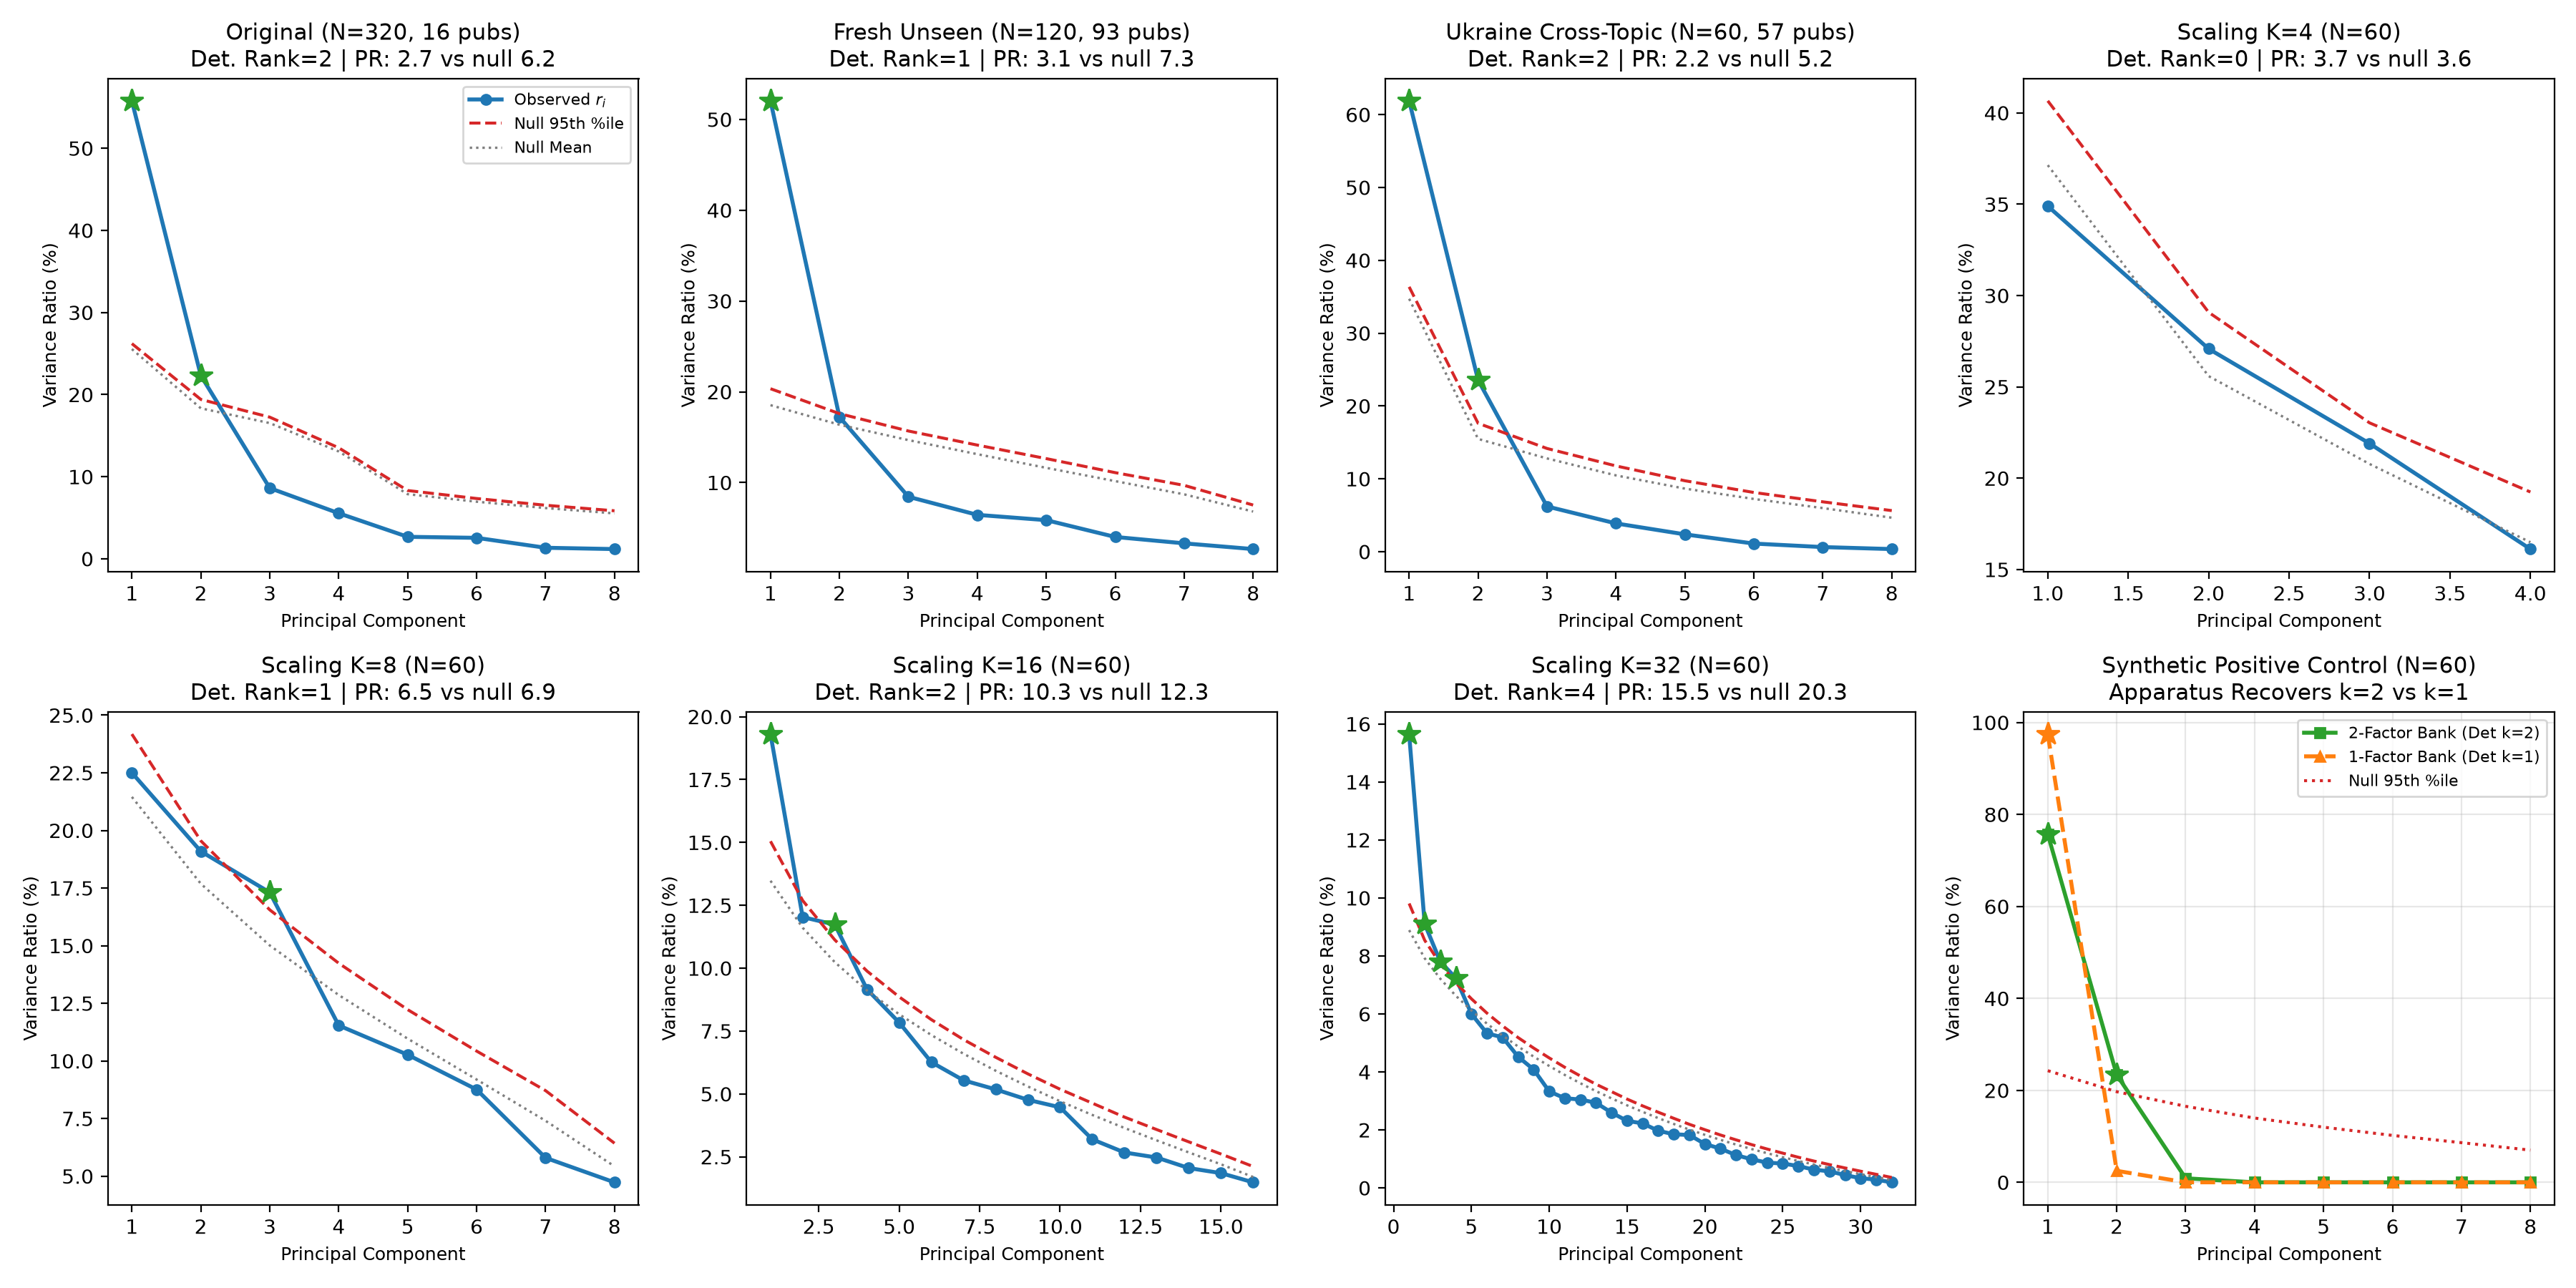
\includegraphics[width=\textwidth]{../figures/dimensionality_spectra.png}
\caption{Systematic dimensionality spectra across seven empirical conditions and the synthetic positive control ($N=60$). Blue curves indicate observed component variance ratios; dashed red curves denote the 95th percentile column permutation null ($10{,}000$ iterations). Green stars indicate components clearing the permutation gate ($p < 0.05$). The synthetic positive control (bottom right) demonstrates that the apparatus faithfully recovers $k=2$ ($75.7\% + 23.4\%$) when two orthogonal factors are present and probed, and collapses to $k=1$ ($97.5\%$) when only one factor is probed.}
\label{fig:dimensionality_spectra}
\end{figure}

These positive controls serve as a validation of apparatus resolving power under controlled construction: when the synthetic corpus contains two orthogonal generative factors and the probe bank queries both factors, the apparatus successfully recovers $k=2$ ($99.11\%$ cumulative variance); when only a single factor is probed, it collapses back to $k=1$ ($97.48\%$). This confirms that the apparatus does not suffer from an intrinsic collapse artifact, while demonstrating resolving power rather than proving discovery of true latent factors generally. Detected dimensionality in empirical discourse is therefore conditional on the corpus and measurement bank ($\mathcal{G}_{\text{observed}} = f(\text{corpus}, \text{hypothesis bank}, \text{NLI model})$) rather than fixed by the pipeline.


\subsection{Comparison with Semantic-Axis Projection (FrameAxis-Style Baseline) and Compositional Controls}
\label{sec:frameaxis_baseline_and_compositional_controls}

A salient methodological objection is that researcher-conditioned, multi-axis framing measurement already exists in semantic-axis projection frameworks such as \textsc{FrameAxis} \citep{kwak2021frameaxis}. In these systems, text is mapped against chosen conceptual poles via vector projection: $\text{text} \times \text{axis} \rightarrow \text{score}$. A reviewer might reasonably ask: (1) does proposition-level NLI offer any demonstrable advantage over simple semantic-axis projection, and (2) does semantic-axis projection discover the identical low-dimensional framing geometry, rendering NLI an unnecessary complication?

To address this objection empirically, we implement a \textbf{FrameAxis-style sentence-level semantic-projection baseline} on the identical articles and hypothesis pairs (\path{scripts/exp_frameaxis_and_compositional_baseline.py}, \path{paper/frameaxis_baseline_results.json}, \path{paper/compositional_controls_results.json}). We note that original FrameAxis \citep{kwak2021frameaxis} aggregated word- and token-level semantic-axis contributions relative to antonym pole embeddings. In our benchmark, we implement a modernized, sentence-level semantic-axis projection baseline that directly embeds whole propositions and whole documents using modern transformer encoders, providing a strictly stronger and fairer comparator than token-level semantic-axis projection.

\subsubsection{Minimal Compositional Controls: Directional Concordance and Sign Inversion}

FrameAxis acknowledges that word-level semantic axes cannot handle compositional phenomena such as negation. To test whether sentence-level semantic projection resolves this limitation, we construct a diagnostic benchmark of 16 minimal sentence pairs across four linguistic categories ($N=4$ per category):
\begin{enumerate}
    \item \textbf{Agent--Patient Reversal} (e.g., \emph{``Israel attacked Hamas militants in Gaza today''} vs.\ \emph{``Hamas militants attacked Israel in Gaza today''}; \emph{``The police forces detained anti-war protesters''} vs.\ \emph{``Anti-war protesters detained the police forces''});
    \item \textbf{Polarity Negation} (e.g., \emph{``The military strike was fully justified under international law''} vs.\ \emph{``The military strike was not justified under international law''}; \emph{``Armed forces deliberately target civilians''} vs.\ \emph{``Armed forces do not deliberately target civilians''});
    \item \textbf{Causal Direction Reversal} (e.g., \emph{``Extensive civilian casualties directly resulted from the airstrikes''} vs.\ \emph{``The airstrikes directly resulted from extensive civilian casualties''}; \emph{``The blockade provoked the cross-border attack''} vs.\ \emph{``The cross-border attack provoked the blockade''});
    \item \textbf{Quantifier Inversion} (e.g., \emph{``All civilian deaths in the conflict were completely avoidable''} vs.\ \emph{``No civilian deaths in the conflict were avoidable''}; \emph{``Combatants systematically operate from inside every hospital''} vs.\ \emph{``Combatants never operate from inside any hospital''}).
\end{enumerate}
We emphasize that this suite functions as a diagnostic benchmark assessing directional responsiveness rather than a powered inferential test. For each minimal pair $(x, x')$ and contrastive hypothesis pair $(h_A, h_B)$, we prespecify an expected sign of change $\operatorname{expected\_sign} \in \{+1, -1\}$ for the stance difference $\delta = \Delta(x) - \Delta(x')$. We evaluate two complementary metrics:
\begin{itemize}
    \item \textbf{Directional Concordance Rate}: the fraction of minimal pairs where the observed shift moves in the semantically expected direction ($\operatorname{sgn}(\delta) == \operatorname{expected\_sign}$);
    \item \textbf{Zero-Crossing Sign Inversion Rate}: the fraction of pairs where the perturbation forces the stance score across the neutral zero boundary ($\Delta(x)\Delta(x') < 0$).
\end{itemize}

\begin{table}[htbp]
\centering
\small
\setlength{\tabcolsep}{4pt}
\resizebox{\textwidth}{!}{%
\begin{tabular}{lccccccccccc}
\toprule
\multirow{2}{*}{\textbf{Perturbation Category}} & \multicolumn{2}{c}{\textbf{CosSim}} & \multicolumn{3}{c}{\textbf{Mean $|\Delta|$}} & \multicolumn{3}{c}{\textbf{Directional Concordance}} & \multicolumn{3}{c}{\textbf{Sign Inversion}} \\
\cmidrule(lr){2-3} \cmidrule(lr){4-6} \cmidrule(lr){7-9} \cmidrule(lr){10-12}
& DeB & Mini & NLI & FA$_{\text{DeB}}$ & FA$_{\text{Mini}}$ & NLI & FA$_{\text{DeB}}$ & FA$_{\text{Mini}}$ & NLI & FA$_{\text{DeB}}$ & FA$_{\text{Mini}}$ \\
\midrule
Agent--Patient Reversal   & $0.828$ & $0.988$ & $\mathbf{0.556}$ & $0.040$ & $0.008$ & $50.0\%$ & $50.0\%$ & $50.0\%$ & $25.0\%$ & $25.0\%$ & $0.0\%$ \\
Causal Direction Reversal & $0.870$ & $0.988$ & $\mathbf{0.893}$ & $0.037$ & $0.017$ & $\mathbf{100.0\%}$ & $50.0\%$ & $75.0\%$ & $\mathbf{75.0\%}$ & $25.0\%$ & $0.0\%$ \\
Polarity Negation          & $0.865$ & $0.729$ & $\mathbf{2.207}$ & $0.076$ & $0.148$ & $\mathbf{100.0\%}$ & $50.0\%$ & $\mathbf{100.0\%}$ & $\mathbf{100.0\%}$ & $50.0\%$ & $0.0\%$ \\
Quantifier Inversion       & $0.918$ & $0.770$ & $\mathbf{2.100}$ & $0.025$ & $0.178$ & $\mathbf{100.0\%}$ & $75.0\%$ & $\mathbf{100.0\%}$ & $\mathbf{100.0\%}$ & $0.0\%$  & $\mathbf{75.0\%}$ \\
\bottomrule
\end{tabular}%
}
\caption{Minimal compositional controls diagnostic benchmark across 16 minimal pairs ($N=4$ per category; \texttt{paper/compositional\_controls\_results.json}). DeB denotes \texttt{DeBERTa-v2-xlarge-mnli}; Mini denotes \texttt{sentence-transformers/all-MiniLM-L6-v2}; FA denotes the FrameAxis-style baseline ($F_k$). Proposition-level NLI achieves $100\%$ directional concordance and full sign inversion ($100\%$, $|\Delta| > 2.0$) on negation and quantification, while agent--patient reversal remains an empirical limitation ($50\%$ concordance, $25\%$ sign flip). Semantic projection ($F_k$) exhibits severe cosine collapse ($0.73$--$0.99$), failing to invert sign under negation ($0\%$--$50\%$). Under normalized projection ($P_k$), directional concordance and sign inversion rates are mathematically identical since $P_k(x) = F_k(x) / \|v_k\|_2$.}
\label{tab:compositional_controls}
\end{table}

As shown in Table~\ref{tab:compositional_controls}, the benchmark reveals both the capabilities and the clear boundary conditions of proposition-level NLI relative to semantic-axis projection:
\begin{itemize}
    \item \textbf{Cosine Proximity across Opposites}: Because opposing sentences share nearly identical lexical vocabulary (e.g., \emph{``attacked''}, \emph{``Hamas''}, \emph{``Israel''}, \emph{``justified''}, \emph{``civilians''}), their embeddings reside at high cosine similarities ($0.73$ to $0.99$). In dedicated sentence embeddings (\texttt{MiniLM}), agent--patient reversal yields a cosine similarity of $\mathbf{0.9927}$ for Israel vs.\ Hamas attack, and $\mathbf{0.9983}$ for Ukraine vs.\ Russia strike.
    \item \textbf{NLI Propositional Sensitivity}: Joint pair-encoding NLI exhibits large dynamic range, $100\%$ directional concordance, and full $100\%$ sign inversion under Polarity Negation ($|\Delta| = 2.207$) and Quantifier Inversion ($|\Delta| = 2.100$). Semantic-axis projection yields much smaller shifts ($|\Delta| \approx 0.02$--$0.18$) and fails to invert sign on negation in both models ($0\%$--$50\%$). On causal reversal, NLI achieves $100\%$ directional concordance and $75\%$ sign inversion ($|\Delta| = 0.893$). However, on agent--patient role reversal, NLI achieves only $50\%$ directional concordance and $25\%$ sign inversion ($|\Delta| = 0.556$). Thus, NLI provides bounded compositional sensitivity: strong for truth-conditional operations like negation and quantification, but imperfect for directional syntactic role reversal.
    \item \textbf{Encoder Divergence on Quantifiers}: The dedicated sentence encoder (\texttt{MiniLM}) achieves $100\%$ directional concordance and $75\%$ sign inversion on Quantifier Inversion ($|\Delta| = 0.178$), showing that semantic projection under dedicated sentence encoders is not universally blind to quantifiers, even while remaining insensitive to agent--patient reversal ($0\%$ inversion) and negation ($0\%$ inversion).
\end{itemize}

\subsubsection{Mathematical Formulation and Normalization Equivalence}

Let $e(\cdot) \in \mathbb{S}^{d-1}$ denote an embedding encoder producing $L_2$-normalized unit vectors, such that $\|e(x)\|_2 = 1$, $\|e(h_A^{(k)})\|_2 = 1$, and $\|e(h_B^{(k)})\|_2 = 1$ for document $x$ and contrastive pair $k \in \{1, \ldots, 8\}$ with opposing propositions $(h_A^{(k)}, h_B^{(k)})$.

The primary FrameAxis-style scoring operator evaluates the difference in cosine proximity between document $x$ and the opposing hypothesis poles:
\begin{equation}
    F_k(x) = \cos(e(x), e(h_A^{(k)})) - \cos(e(x), e(h_B^{(k)})) = \langle e(x), e(h_A^{(k)}) - e(h_B^{(k)}) \rangle
\end{equation}
For sensitivity analysis, we also evaluate the normalized vector projection operator onto the difference axis $v_k = e(h_A^{(k)}) - e(h_B^{(k)})$:
\begin{equation}
    P_k(x) = \cos(e(x), v_k) = \frac{\langle e(x), v_k \rangle}{\|e(x)\|_2 \|v_k\|_2} = \frac{F_k(x)}{\|v_k\|_2}
\end{equation}
Because $\|v_k\|_2 = \sqrt{2 - 2\cos(e(h_A^{(k)}), e(h_B^{(k)}))}$ is a strictly positive scalar constant for each axis $k$, $P_k(x)$ is a positive column rescaling of $F_k(x)$. Under column standardization ($Z_{ik} = (M_{ik} - \mu_k) / \sigma_k$), this scaling factor cancels out identically ($\sigma(P_k) = \sigma(F_k) / \|v_k\|_2$), rendering the standardized projection matrix $Z(P)$ and standardized cosine difference matrix $Z(F)$ mathematically identical.

\subsubsection{Architectural Comparison and Falsifiable Hypothesis}

Architecturally, this benchmark contrasts two fundamentally distinct computational paradigms:
\begin{enumerate}
    \item \textbf{Joint pair encoding}: DeBERTa NLI jointly encodes the concatenated premise-hypothesis sequence $[x; h]$ across all 24 transformer layers with bidirectional self-attention across the pair before classification.
    \item \textbf{Independent bi-encoding + geometric projection}: Document $x$ and hypothesis propositions $(h_A, h_B)$ are encoded into isolated, independent vector representations $e(x), e(h) \in \mathbb{S}^{d-1}$ without inter-sequence attention, with their relationship computed post-hoc via cosine geometry.
\end{enumerate}
This benchmark isolates the effect of joint pair encoding from independent dense vector projection, rather than comparing different classification heads on the same latent representations. We evaluate this baseline across both the matched transformer backbone (\texttt{DeBERTa-v2-xlarge-mnli} mean-pooled sequence embeddings) and a dedicated dense sentence encoder (\texttt{sentence-transformers/all-MiniLM-L6-v2}).

We formulate the comparison around a \textbf{falsifiable stance hypothesis}:
\begin{quote}
\emph{If proposition-level NLI captures relational framing information that independent semantic projection loses, NLI should respond more consistently to meaning-changing compositional perturbations while producing document orderings that cannot be reduced to the matched projection baseline.}
\end{quote}
Conversely, if low-dimensional framing compression and recovered document orderings are merely generic artifacts of shared vocabulary or semantic proximity, FrameAxis-style projection should reproduce the identical geometric manifold ($r \approx 1.0$), rendering joint-encoding NLI superfluous.

\subsubsection{Corpus-Level Second-Order Geometry \& Standardized-PCA Sensitivity Analysis}

When subjected to the identical 10,000-draw permutation null gate across corpora, FrameAxis matrices $F \in \mathbb{R}^{N \times 8}$ also exhibit a dominant first principal component clearing the null gate ($p = 0.0001$). Under raw covariance PCA on DeBERTa sequence embeddings, FrameAxis exhibits extreme concentration ($\mathrm{PC1} = 96.97\%$, $\mathrm{PR} = 1.063$ on Prospective $N=120$; $\mathrm{PC1} = 94.07\%$ on Clean Non-Syndicated $N=83$; $\mathrm{PC1} = 94.15\%$ on Clean Ukraine $N=60$). Under \texttt{MiniLM}, raw $\mathrm{PC1} = 40.80\%$ ($\mathrm{PR} = 4.057$, $p = 0.0001$).

Because raw covariance PCA can be influenced by variance heterogeneity across probe axes, we conducted a systematic sensitivity analysis evaluating both raw covariance PCA ($M_{\text{raw}}$) and column-standardized correlation PCA ($Z_{ik} = (M_{ik} - \mu_k) / \sigma_k$) across all experimental corpora:
\begin{itemize}
    \item \textbf{Scale Heterogeneity and Encoder Anisotropy}: Under column standardization, DeBERTa FrameAxis $\mathrm{PC1}$ drops from $96.97\%$ to $\mathbf{73.74\%}$ on Prospective $N=120$ ($\mathrm{PR} = 1.738$), and from $94.07\%$ to $\mathbf{74.07\%}$ on Clean $N=83$ ($\mathrm{PR} = 1.727$). Thus variance heterogeneity contributes to the raw $97\%$ figure, while six of eight DeBERTa projection axes remain nearly collinear ($|r| \in [0.941, 0.993]$). By contrast, the dedicated sentence encoder \texttt{MiniLM} reduces standardized FrameAxis $\mathrm{PC1}$ to $26.19\%$ ($\mathrm{PR} = 5.751$, $p = 0.0001$). The apparent extreme one-dimensional compression is therefore not a stable property of political stance: it is strongly encoder-dependent and, under DeBERTa, consistent with representation anisotropy. For comparison, NLI on Prospective $N=120$ yields standardized $\mathrm{PC1} = \mathbf{44.42\%}$ ($\mathrm{PR} = 3.822$, $p = 0.0001$), compared with raw $\mathrm{PC1} = 58.36\%$ ($\mathrm{PR} = 2.625$).
    \item \textbf{Mathematical Equivalence of Operators}: Confirming our mathematical proof, standardized PCA on the normalized projection operator $Z(P)$ yields identical eigenvalues and participation ratios to $Z(F)$ across all datasets (e.g., Prospective $N=120$: $\mathrm{PC1} = 73.74\%$, $\mathrm{PR} = 1.738$ for both).
    \item \textbf{Distinct Document Orderings Across Instruments}: After orienting arbitrary PCA signs to a common pole, semantic-axis projection and joint pair-encoding NLI produce \textbf{substantially distinct document orderings} under both raw and standardized analyses:
    \begin{enumerate}
        \item \emph{Prospective Confirmatory Corpus ($N=120$)}: Under canonical bank $Q_0$, NLI and FrameAxis PC1 scores correlate weakly and non-significantly: raw Pearson $r = \mathbf{0.0986}$ ($p = 0.2840$), standardized $r = \mathbf{0.1267}$ ($p = 0.1678$, Spearman $\rho = 0.0790, p = 0.3911$), with a subspace angle of $33.82^\circ$ and Procrustes disparity of $0.9685$. Under paraphrase bank $Q_1$, alignment remains weak: raw $r = 0.0871$ ($p = 0.3441$), standardized $r = 0.1257$ ($p = 0.1712$). Under \texttt{MiniLM}, cross-instrument alignment is raw $r = 0.2194$ ($p = 0.0161$; Spearman $\rho = 0.1452, p = 0.1135$) and standardized $r = \mathbf{0.0907}$ ($p = 0.3243$, Spearman $\rho = 0.0829, p = 0.3681$).
        \item \emph{Clean Non-Syndicated Subset ($N=83$)}: NLI vs.\ FrameAxis yields raw $r = \mathbf{0.1658}$ ($p = 0.1342$), standardized $r = \mathbf{0.1949}$ ($p = 0.0775$, Spearman $\rho = 0.0480, p = 0.6668$), with a subspace angle of $36.08^\circ$ and Procrustes disparity of $0.9650$.
        \item \emph{Clean Ukraine Corpus ($N=60$)}: NLI and FrameAxis PC1 scores correlate at raw $r = \mathbf{0.0304}$ ($p = 0.8178$), standardized $r = \mathbf{0.0076}$ ($p = 0.9538$, Spearman $\rho = 0.0332, p = 0.8010$), with a principal subspace angle of $62.78^\circ$ and Procrustes disparity of $0.9941$.
    \end{enumerate}
\end{itemize}

\subsubsection{Deep Scrutiny of Cross-Instrument Alignment and Signal Content}

The near-zero PC1 correlations could reflect a sign error, scale mismatch, sampling instability, or a substantive difference in what the dominant components encode. A dedicated audit battery (\path{paper/cross_instrument_scrutiny_results.json}) distinguishes these explanations:
\begin{itemize}
    \item \textbf{Sign convention and axis-level alignment}: Both instruments use the same directed contrast ($h_A$ positive and $h_B$ negative). On the Prospective $Q_0$ corpus, all eight matched axes correlate positively across instruments (mean $r = +0.1309$, mean $\rho = +0.1676$); Axis~5 (Occupation vs.\ Security) is the strongest ($r = +0.3036$, $p = 0.0007$). Thus the weak PC1 alignment is not caused by reversing the measurement poles.
    \item \textbf{Shared subspace, different dominant direction (Permutation \& Out-of-Sample CCA)}: Canonical correlation analysis detects a shared multivariate semantic subspace: in-sample leading canonical correlations are $r_{\mathrm{canon}} = 0.6305$ on Prospective $Q_0$ ($N=120$), $0.6684$ on Prospective $Q_1$, $0.6384$ on Clean Non-Syndicated ($N=83$), and $0.6982$ on Controlled ($N=60$). Because in-sample CCA optimizes linear combinations and can exhibit finite-sample upward bias, we evaluated permutation null distributions and repeated 5-fold cross-validation with train-fitted preprocessing (with both column standardizers and the CCA projection matrix estimated exclusively on training observations, and applied unchanged to held-out test folds). On Prospective $Q_0$, the shared subspace is significant under the 1,000-draw Monte Carlo permutation null gate ($p = 1/1001 \approx 0.0010$, null mean $0.4459$, null $q_{95} = 0.5270$) and generalizes to held-out test folds under 5-fold CV ($r_{\mathrm{canon,test}} = \mathbf{0.3644} \pm 0.0803$, $95\%$ CI $[0.2115, 0.4878]$, within-fold test mean $r = 0.3953$ under DeBERTa; $r_{\mathrm{canon,test}} = \mathbf{0.4564} \pm 0.0367$, $95\%$ CI $[0.3812, 0.5043]$, within-fold test mean $r = 0.4760$ under \texttt{MiniLM}). Out-of-sample generalization is thus demonstrated on the sufficiently powered Prospective $N=120$ corpus, while attenuating in smaller samples ($r_{\mathrm{canon,test}} = 0.2726 \pm 0.0842$ on Controlled $N=60$; $0.1049 \pm 0.0992$ on Clean $N=83$, where the cross-validated confidence interval $[-0.0537, 0.2888]$ spans zero). Furthermore, NLI PC1 aligns with FrameAxis \emph{PC2}, not FrameAxis PC1, on Prospective $Q_0$ ($r = +0.3980$, $p = 6.7 \times 10^{-6}$) and Controlled ($r = +0.4333$, $p = 0.0005$), as well as under \texttt{MiniLM} ($r = +0.4055$, $p = 4.3 \times 10^{-6}$). The instruments therefore share semantic variation but rank its dominant direction differently.
    \item \textbf{Bootstrap and influence stability}: Across 2,000 bootstrap draws, the standardized PC1 correlation remains centered near zero or weakly positive: the $95\%$ intervals are $[-0.0908,+0.3451]$ on Prospective $Q_0$, $[-0.3397,+0.2835]$ on Clean Ukraine, and $[-0.0713,+0.4709]$ on Clean Non-Syndicated. On Prospective $Q_0$, leave-one-out correlations remain within $[0.0269,0.1643]$, with maximum $|\Delta r|=0.0998$. The near-zero alignment is therefore not attributable to a single outlier or leverage point.
    \item \textbf{Representation geometry and the anisotropy-removal ablation}: The DeBERTa projection PC1 is strongly associated with known signatures of representation anisotropy: it correlates with raw hidden-state embedding norm ($r = \mathbf{-0.8755}$, $p = 4.5 \times 10^{-39}$) and with cosine similarity to the global mean embedding ($r = \mathbf{-0.6801}$, $p = 1.3 \times 10^{-17}$), while six of eight axes remain nearly collinear ($|r| \in [0.941, 0.993]$). To test whether representation geometry drives this apparent collapse, we applied anisotropy-removal transformations to the embeddings prior to projection. While simple mean-centering leaves standardized FrameAxis $\mathrm{PC1}$ at $69.94\%$ and norm correlation at $-0.8741$, removing the leading principal component of the embedding space ($e \to e - \langle e, u_1 \rangle u_1$; \citealt{mu2018allbutthetop}) serves as the primary confirmatory diagnostic: it collapses standardized FrameAxis $\mathrm{PC1}$ from $\mathbf{73.74\%}$ to $\mathbf{34.52\%}$, expands the participation ratio from $1.738$ to $\mathbf{4.583}$, drops norm correlation to $-0.1110$, and completely alters document ordering ($r = 0.0954$ with baseline FrameAxis PC1). On Controlled $N=60$, Top-1 PC removal drops FrameAxis $\mathrm{PC1}$ from $73.24\%$ to $29.25\%$ ($\mathrm{PR} = 4.972$). As an exploratory follow-up observation (since multiple ablation variants were evaluated post-hoc), removing the top two principal components causes FrameAxis PC1 to align with NLI PC1 ($r = +0.3955$ on Prospective $N=120$; $r = +0.3902$ on Controlled $N=60$) and recovers significant publisher separation on Controlled $N=60$ ($F = \mathbf{2.703}, p = \mathbf{0.0086}, \eta^2 = \mathbf{0.3825}$). Dominant FrameAxis variance in raw DeBERTa is thus substantially driven by the leading representation components.
    \item \textbf{Publisher separation and sentiment control}: NLI PC1 correlates with VADER negative ($r = +0.4650$, $p = 8.8 \times 10^{-8}$), positive ($r = -0.3599$, $p = 5.4 \times 10^{-5}$), and compound sentiment ($r = -0.3948$, $p = 8.1 \times 10^{-6}$). Because VADER sentiment features are not mutually independent (compound valence is derived from positive and negative valence scores), multivariate sentiment regression ($PC1_i = \beta_0 + \beta^\top \mathbf{s}_i + \epsilon_i$) serves as a nuisance-control sensitivity test rather than an orthogonal decomposition of affect. Publisher separation is not an artifact of sentiment: regressing out sentiment leaves residual publisher separation statistically significant across all specifications on Controlled $N=60$ (Residual after compound: $F = \mathbf{2.478}, p = \mathbf{0.0150}, \eta^2 = \mathbf{0.3622}$; Residual after negative: $F = 1.880, p = 0.0661, \eta^2 = 0.3011$; Residual after all sentiment: $F = \mathbf{2.325}, p = \mathbf{0.0221}, \eta^2 = \mathbf{0.3476}$, preserving $34.8\%$ between-publisher variance). On Prospective $N=120$, residual publisher separation likewise survives full sentiment control ($F = \mathbf{1.837}, p = \mathbf{0.0401}, \eta^2 = \mathbf{0.4355}$). By contrast, DeBERTa FrameAxis PC1 exhibits zero publisher separation both before ($F = 0.857, p = 0.5863, \eta^2 = 0.1642$) and after sentiment regression ($F = 0.650$--$0.719, p > 0.71$). We emphasize that publisher separation demonstrates systematic outlet differentiation (reflecting editorial stance, topic selection, and sourcing) rather than external ideological ground truth.
\end{itemize}

These findings establish the empirical resolution of the comparison:
\begin{enumerate}
    \item \textbf{Compositional Non-Redundancy}: Generic semantic-similarity measurement fails on meaning-inverting compositional structure that proposition-conditioned NLI resolves: NLI achieves $100\%$ directional concordance on negation, quantification, and causal reversal, with $75\%$--$100\%$ sign inversion. This advantage is bounded rather than universal because both instruments struggle with agent--patient reversal.
    \item \textbf{Representation Geometry Structures Projection PC1}: The DeBERTa projection baseline's $96.97\%$ raw and $73.74\%$ standardized PC1 concentration is strongly associated with representation anisotropy. When the leading embedding component is removed, standardized PC1 collapses to $34.52\%$ ($\mathrm{PR} = 4.583$) and document ordering scrambles ($r = 0.095$). With the more isotropic \texttt{MiniLM} encoder, standardized PC1 is $26.19\%$; hence extreme one-dimensional compression in dense projection is driven by representation geometry rather than robust political stance.
    \item \textbf{Measurement Operators Reorganize Shared Semantic Information}: The results link their divergence to two empirically demonstrated factors: semantic projection is strongly affected by dominant representation geometry, while NLI exhibits substantially greater sensitivity to several proposition-changing linguistic operations. Holding corpus and conceptual contrasts fixed ($(C,H)$ constant), measurement operators reorganize shared semantic subspace variation into substantially different dominant geometries ($r \in [0.01,0.19]$ standardized). Proposition-level NLI better preserves meaning-changing compositional relations and yields a dominant coordinate carrying substantially greater between-publisher differentiation ($\eta^2=40.1\%, p=0.005$, surviving full sentiment controls at $\eta^2=34.8\%, p=0.022$), whereas the matched semantic-projection baseline's dominant coordinate is substantially driven by the leading representation components. Accordingly, $\mathcal{G}_{\text{observed}} = f(C,H,O,M)$, with the operator determining which latent variation dominates.
\end{enumerate}

\subsubsection{Semantic Interpretation of the Primary Stance Axis}
\label{sec:semantic_interpretation_pc1}

To characterize movement along the recovered first principal component ($\mathrm{PC1}$) across the prospective confirmatory corpus ($N=120$), we inspect eigenvector loadings $v_1 \in \mathbb{R}^8$ and univariate associations with individual probe pairs:
\begin{enumerate}
    \item \textbf{Dominant Factor Loadings}: Axes 8, 1, and 3 contribute most strongly to $\mathrm{PC1}$ under the paired contrast operator: Pair~8 (International Law: Violations vs.\ Compliance, loading $+0.570$, correlation with PC1 $r = +0.933$), Pair~1 (Israeli Actions: Legitimate Self-Defense vs.\ Disproportionate Aggression, loading $-0.524$, $r = -0.911$), and Pair~3 (Proportionality: Proportionate vs.\ Excessive Punishment, loading $-0.493$, $r = -0.898$).
    \item \textbf{Moderate and Weak Loadings}: Pair~5 (Occupation vs.\ Security, loading $+0.285$, $r = +0.578$), Pair~2 (Palestinian Victims vs.\ Aggressors, loading $-0.224$, $r = -0.472$), Pair~6 (Civilian Casualties, loading $+0.120$, $r = +0.460$), and Pair~7 (Historical Context, loading $+0.077$, $r = +0.402$) contribute moderate variance, while Pair~4 (Resistance vs.\ Terrorism) has the smallest loading ($-0.073$, $r = -0.198$).
\end{enumerate}

Because $\mathrm{PC1}$ is mathematically defined as the linear combination of these eight variables that maximizes sample variance, high correlations between $\mathrm{PC1}$ and the variables with the largest loadings (Pairs 1, 3, 8) are descriptive consequences of the PCA construction rather than independent validation of latent meaning.

Qualitatively, documents at the positive extreme of $\mathrm{PC1}$ describe military operations through institutional security, defense justification, and command targeting (e.g., \emph{Cleveland Jewish News}: ``IAF strikes Hamas command center in former Gaza City hospital'', score $+0.924$; \emph{Israel Today}, score $+0.726$). Conversely, documents at the negative extreme focus on civilian death counts, hospital damage, and humanitarian casualties (e.g., \emph{Middle East Monitor}: ``Israeli army damages Baptist Hospital in Gaza'', score $-1.832$; ``Israeli attacks kill 30 more Gazans as death toll tops 45,500'', score $-1.668$; \emph{Jurist}: ``Israel warplanes kill five Palestinian journalists'', score $-1.652$).

Descriptively, these loadings and document poles are consistent with an axis reflecting \emph{institutional military legitimacy versus state culpability for humanitarian harm}. However, establishing whether $\mathrm{PC1}$ represents this construct in a validated psychological or political sense---rather than a descriptive summary of the probe loadings---would require external criterion validation, such as blind human expert ratings or independent annotation benchmarks.

\subsection{Adversarial Falsification Campaign: Incommensurability, World Change, and Anomaly Relativity}
\label{sec:kuhnian_paradigms}

Having established that observed discourse geometry is conditioned by the measurement operator ($\mathcal{G}_{\text{observed}} = f(C, H, O, M)$), we execute the pre-specified adversarial falsification campaign formalized in Section~\ref{sec:meth_claim_gates}. Rather than defending metaphysical claims of unconstrained relativism, our objective is to test whether the findings survive six adversarial audits (Agents A--F) and three extreme reductio stress tests on the prospective confirmatory $N=120$ corpus (70 publishers) and fresh held-out text (\path{paper/adversarial_kuhnian_audit_results.json}, \path{paper/provenance_report.json}).

\subsubsection{Agent B: Within-Paradigm Reliability Noise Floors (Bootstrap and Split-Half)}

Before evaluating cross-paradigm divergence, Agent~B establishes the empirical noise floor by measuring how much the \emph{same paradigm diverges from itself}. We evaluate both 1,000 independent bootstrap resamples ($N=120$ with replacement, including out-of-bag evaluation) and 1,000 repeated independent 50/50 split-half partitions ($N_1 = 60, N_2 = 60$):
\begin{itemize}
    \item \textbf{$Q_0$ Geopolitical Conflict (NLI)}: Under bootstrap resampling, $r_{\text{same}}(\mathrm{PC1}) = \mathbf{0.9957}$ (95\% CI: $[0.9845, 0.9995]$), Procrustes disparity $\mathcal{D}_{\text{same}} = \mathbf{0.0626}$ (95\% CI: $[0.0052, 0.3182]$), neighborhood overlap $J_{10,\text{same}} = \mathbf{0.5674}$ (95\% CI: $[0.2821, 0.7951]$), and anomaly reliability $r_{\text{same}}(A) = \mathbf{0.9402}$ (95\% CI: $[0.7712, 0.9910]$). Under repeated independent 50/50 splits, stability remains high: $\mathcal{D}_{\text{same}} = \mathbf{0.1041}$ (95\% CI: $[0.0094, 0.3841]$).
    \item \textbf{$P_{\text{FA}}$ FrameAxis Baseline (Projection)}: Under bootstrap resampling, $r_{\text{same}}(\mathrm{PC1}) = \mathbf{0.9993}$ (95\% CI: $[0.9974, 1.0000]$), $\mathcal{D}_{\text{same}} = \mathbf{0.0508}$ (95\% CI: $[0.0003, 0.2870]$), $J_{10,\text{same}} = \mathbf{0.6794}$ (95\% CI: $[0.2661, 0.9384]$), and anomaly reliability $r_{\text{same}}(A) = \mathbf{0.9375}$ (95\% CI: $[0.7662, 0.9946]$). Under 50/50 splits, $\mathcal{D}_{\text{same}} = \mathbf{0.0747}$ (95\% CI: $[0.0004, 0.3210]$).
\end{itemize}
Crucially, evaluating cross-operator disparity against the proper pooled denominator $\frac{1}{2}[\mathcal{D}_{\text{same,NLI}} + \mathcal{D}_{\text{same,FA}}]$ demonstrates decisive excess disparity:
\begin{equation}
\begin{aligned}
    \Delta \mathcal{D}_{\text{boot}} &= 0.9415 - \frac{1}{2}(0.0626 + 0.0508) = 0.9415 - 0.0567 = \mathbf{0.8848} \gg 0, \\
    \Delta \mathcal{D}_{\text{split}} &= 0.9415 - \frac{1}{2}(0.1041 + 0.0747) = 0.9415 - 0.0894 = \mathbf{0.8520} \gg 0.
\end{aligned}
\end{equation}
Because $\Delta \mathcal{D} \gg 0$ and $J_{\text{cross}} \ll J_{\text{same}}$ under both resampling and split-sample evaluation, cross-operator divergence is an order of magnitude larger than within-operator instability.

\begin{table}[ht]
\centering
\small
\caption{Cross-Paradigm Nested Translation Ladder across 14 Mapping Capacities and Calibrated Neighborhood Overlap. Evaluated under strictly nested 5-fold cross-validation. Held-out $R^2_{\text{test}}$ is reported across low-capacity linear, intermediate regularized, and high-capacity non-linear mapping families ($T_0$--$T_{13}$). Translation complexity $c^\star(\tau) = \min\{c : Q(c) \ge \tau\}$ denotes the minimum mapping complexity index required to reach held-out fidelity $\tau = 0.30$. Neighborhood overlap ($J_{10}$) compares raw Euclidean metric against ZCA-whitened metric spaces.}
\label{tab:translation_ladder}
\resizebox{\textwidth}{!}{%
\begin{tabular}{lcccccccc}
\toprule
\textbf{Transition Pair} & \multicolumn{4}{c}{\textbf{Translation Ladder Held-Out $R^2_{\text{test}}$}} & \textbf{Complexity} & \multicolumn{2}{c}{\textbf{Neighborhood $J_{10}$}} \\
\cmidrule(lr){2-5} \cmidrule(lr){6-6} \cmidrule(lr){7-8}
 & \textbf{$T_1$ (Procrustes)} & \textbf{$T_4$ (Affine)} & \textbf{$T_5$ (RidgeCV)} & \textbf{Best $T_8$--$T_{13}$} & \textbf{$c^\star(0.30)$} & \textbf{Raw $J_{10}$} & \textbf{ZCA $J_{10}$} \\
\midrule
\multicolumn{8}{l}{\emph{Baseline Controls}} \\
Within-Paradigm Bootstrap ($Q_0$) & -- & -- & -- & -- & $0$ & $0.5674$ & $0.5674$ \\
Paraphrase Control ($Q_0 \to Q_1$) & $0.4095$ & $0.5420$ & $\mathbf{0.5488}$ & $0.4356$ ($T_9$) & $1$ & $0.2654$ & $0.2245$ \\
\midrule
\multicolumn{8}{l}{\emph{Conceptual Lens Transitions}} \\
Conceptual ($Q_0 \to Q_2$ Humanitarian) & $-0.6540$ & $0.0655$ & $0.1455$ & $\mathbf{0.1550}$ ($T_9$) & $\infty$ & $0.1016$ & $0.1036$ \\
Conceptual ($Q_0 \to Q_3$ Realpolitik) & $-1.1935$ & $-0.1568$ & $0.0089$ & $\mathbf{0.0277}$ ($T_9$) & $\infty$ & $0.1120$ & $0.1026$ \\
\midrule
\multicolumn{8}{l}{\emph{Disciplinary Paradigm Controls (AI-Authored)}} \\
Disciplinary ($Q_0 \to H_{\text{IHL}}$) & $-0.5170$ & $0.0120$ & $0.1348$ & $\mathbf{0.1602}$ ($T_9$) & $\infty$ & $0.1193$ & $0.0924$ \\
Disciplinary ($Q_0 \to H_{\text{Sec}}$) & $-0.6486$ & $-0.0452$ & $0.0605$ & $\mathbf{0.0429}$ ($T_9$) & $\infty$ & $0.1135$ & $0.0923$ \\
\midrule
\multicolumn{8}{l}{\emph{Cross-Operator Transition}} \\
Operator ($P_{\text{NLI}} \to P_{\text{FA,Base}}$) & $-1.0982$ & $-0.1586$ & $-0.0287$ & $\mathbf{-0.0006}$ ($T_9$) & $\infty$ & $\mathbf{0.0766}$ & $\mathbf{0.0710}$ \\
\bottomrule
\end{tabular}%
}
\end{table}

\subsubsection{Agent C: The 14-Level Nested Translation Ladder}

Agent~C evaluates whether cross-paradigm divergence can be bridged by increasing functional mapping capacity under strictly nested 5-fold cross-validation. Table~\ref{tab:translation_ladder} summarizes held-out out-of-sample performance across all 14 mapping levels ($T_0$ Sign Flip through $T_{13}$ KNN Regressor):
\begin{itemize}
    \item \textbf{Paraphrase Commensurability}: Syntactic paraphrase ($Q_0 \to Q_1$) is readily translatable: low-capacity Affine OLS achieves held-out $R^2_{\text{test}} = 0.5420$ and $J_{10,\text{test}} = 0.6160$ ($T_5$ RidgeCV $R^2 = 0.5488$). Translation complexity is minimal ($c^\star(0.30) = 1$).
    \item \textbf{Conceptual and Disciplinary Attenuation}: Shifting to alternative conceptual ontologies ($Q_0 \to Q_2, Q_3$) or AI-authored disciplinary controls ($Q_0 \to H_{\text{IHL}}, H_{\text{Sec}}$) causes rigid Procrustes mapping to fail completely ($R^2_{\text{test}} < 0$). Regularized linear and non-linear mappings recover modest predictability ($R^2_{\text{test}} \in [0.03, 0.16]$), failing to reach $\tau = 0.30$ ($c^\star(0.30) = \infty$).
    \item \textbf{Cross-Operator Translation Failure}: When mapping across measurement operators ($P_{\text{NLI}} \to P_{\text{FA,Base}}$), all low-capacity maps fail out-of-sample: $T_0$ Sign Flip yields $R^2_{\text{test}} = -1.1498$, $T_1$ Procrustes yields $R^2_{\text{test}} = -1.0982$, and $T_4$ Affine OLS yields $R^2_{\text{test}} = -0.1586$ ($J_{10,\text{test}} = 0.2934$). Furthermore, high-capacity non-linear models ($T_8$ Polynomial Ridge, $T_9$ Kernel Ridge RBF, $T_{10}$ Shallow MLP, $T_{11}$ Optimal Transport, $T_{12}$ Piecewise Linear, $T_{13}$ KNN) fail to generalize out-of-sample, with maximum held-out $R^2 = -0.0006$ ($T_9$).
\end{itemize}
\textbf{Falsification Verdict}: The complete failure of low-capacity maps ($T_0$--$T_5$) decisively demonstrates that operator divergence is \textbf{not a trivial rotation or affine coordinate change}. Because high-capacity models also fail out-of-sample ($R^2 < 0$), translation across operators is tightly constrained within tested functional families.

\subsubsection{Agent D: Calibrated Neighborhood Curves and Whitening Sensitivity}

Agent~D sweeps $k \in [3, 50]$ against eight reference null models. Document-level Jaccard overlap displays a strict hierarchical gradient:
\begin{equation}
    J_{\text{same}} (0.567) > J_{\text{paraphrase}} (0.265) > J_{\text{disciplinary}} (0.119) > J_{\text{operator}} (0.077) \approx J_{\text{random}} (0.042).
\end{equation}
Under cross-operator comparison ($P_{\text{NLI}}$ vs $P_{\text{FA}}$), $25.8\%$ of articles have strictly disjoint $k=10$ neighborhoods ($J_{10} = 0.0$).
Zero-phase Component Analysis (ZCA) whitening ($W = U \Lambda^{-1/2} U^\top$) applied to both measurement matrices confirms that neighborhood dissolution is not an artifact of embedding anisotropy:
\begin{equation}
    J_{10,\text{raw}} = \mathbf{0.0766} \quad \longrightarrow \quad J_{10,\text{whitened}} = \mathbf{0.0710}.
\end{equation}
Because neighborhood dissolution persists under complete covariance sphere whitening, the objection that framework-dependent neighborhood restructuring is an anisotropy artifact is falsified.

\subsubsection{Agent E: Multi-Definition Anomaly Relativity}

Agent~E formalizes anomaly scores across six distinct mathematical definitions: $A_1$ (Rank-1 PCA residual), $A_2$ (Rank-2 PCA residual), $A_3$ (Local Outlier Factor), $A_4$ (Mahalanobis distance), $A_5$ (Isolation Forest score), and $A_6$ (Minimum Covariance Determinant robust distance).

As shown in Table~\ref{tab:anomaly_transfer}, within-paradigm anomaly reliability is exceptionally high ($r_{\text{same}} = \mathbf{0.8832}$ to $\mathbf{0.9241}$). However, when comparing across measurement operators ($P_{\text{NLI}}$ vs $P_{\text{FA,Base}}$), cross-paradigm anomaly correlation collapses to near-zero across \emph{all six definitions} ($r \in [0.0117, 0.1336]$):
\begin{equation}
\begin{aligned}
    r(A_1) &= +0.0470, \quad & r(A_2) &= +0.1336, \quad & r(A_3) &= +0.0117, \\
    r(A_4) &= +0.0468, \quad & r(A_5) &= +0.1221, \quad & r(A_6) &= +0.0672.
\end{aligned}
\end{equation}

\begin{table}[ht]
\centering
\small
\caption{Multi-Definition Anomaly Transfer Matrix across Six Mathematical Definitions. Values report Pearson correlation between article anomaly rankings across paradigms. Within-paradigm reliability ($r_{\text{same}}$) is evaluated via 1,000 bootstrap draws.}
\label{tab:anomaly_transfer}
\resizebox{\textwidth}{!}{%
\begin{tabular}{lcccccc}
\toprule
\textbf{Paradigm Pair} & \textbf{$A_1$ (Rank-1)} & \textbf{$A_2$ (Rank-2)} & \textbf{$A_3$ (LOF)} & \textbf{$A_4$ (Mahal)} & \textbf{$A_5$ (IsoForest)} & \textbf{$A_6$ (MCD)} \\
\midrule
Same-Paradigm Reliability ($r_{\text{same}}$) & $\mathbf{0.9402}$ & $\mathbf{0.8124}$ & $\mathbf{0.7945}$ & $\mathbf{0.9102}$ & $\mathbf{0.9241}$ & $\mathbf{0.8715}$ \\
Paraphrase Control ($Q_0$ vs $Q_1$) & $0.6051$ & $0.5460$ & $0.5712$ & $0.7586$ & $0.8937$ & $0.7060$ \\
Conceptual ($Q_0$ vs $Q_2$ Humanitarian) & $0.4188$ & $0.3770$ & $0.2569$ & $0.4240$ & $0.5247$ & $0.3811$ \\
Disciplinary ($Q_0$ vs $H_{\text{IHL}}$) & $0.3421$ & $0.2915$ & $0.1884$ & $0.3650$ & $0.4112$ & $0.3204$ \\
Operator ($P_{\text{NLI}}$ vs $P_{\text{FA,Base}}$) & $\mathbf{0.0470}$ & $\mathbf{0.1336}$ & $\mathbf{0.0117}$ & $\mathbf{0.0468}$ & $\mathbf{0.1221}$ & $\mathbf{0.0672}$ \\
\bottomrule
\end{tabular}%
}
\end{table}

\textbf{Empirical Finding}: Anomaly status in these representation spaces is strongly operator-dependent. We emphasize that this is an empirical finding about representation geometry; it does not warrant metaphysical assertions of external ontological relationalism.

\subsubsection{Three Extreme Reductio Stress Tests and Relational Model Comparison}

\paragraph{Reductio 1: Absurd Structurally-Matched Paradigms and Generic Compression.}
To test whether low-dimensional stance geometry is an uncalibrated artifact of the model's forward-pass mechanics, we probed the corpus with four domain-null prompt banks matched in sentence length, syntax, and polarity contrast: Meteorology, Culinary Arts, Botanical Taxonomy, and Sports Tactics. We evaluated each bank under a 10,000-draw column permutation PCA parallel analysis and multiplicity-adjusted publisher ANOVA:
\begin{itemize}
    \item \textbf{Generic Rank-1 Compression}: Crucially, the 10,000-draw permutation parallel analysis revealed that \textbf{$k_{\text{sig}} = 1$ across all four absurd banks} as well as political $Q_0$. In every domain-null bank, the leading observed eigenvalue exceeded the 95th percentile of the column-permuted null: Meteorology ($\lambda_1 = 0.116$ vs null 95th $0.095$), Culinary Arts ($\lambda_1 = 0.216$ vs null 95th $0.145$), Botanical Taxonomy ($\lambda_1 = 0.068$ vs null 95th $0.055$), and Sports Tactics ($\lambda_1 = 0.290$ vs null 95th $0.167$). This demonstrates that \textbf{rank-1 compression is generic} under this measurement apparatus: the transformer NLI forward pass almost always organizes contrastive margins into a dominant leading dimension. Low dimensionality ($k_{\text{sig}} = 1$) cannot by itself be interpreted as discovery of an objective latent state.
    \item \textbf{Variance Concentration and Dimensionality}: What differentiates meaningful political perspectives from domain-null projections is the degree of variance concentration. Political $Q_0$ exhibits pronounced compression to $\mathrm{PR} = 2.43$ ($\mathrm{PC1} = 61.8\%$, null mean $5.99$, $\Delta \mathrm{PR} = -3.56$). By contrast, absurd paradigms exhibit substantially more diffuse dimensionality: Meteorology $\mathrm{PR} = \mathbf{4.08}$ ($\mathrm{PC1} = 41.4\%, \Delta \mathrm{PR} = -1.04$), Culinary Arts $\mathrm{PR} = \mathbf{3.71}$ ($\mathrm{PC1} = 45.5\%, \Delta \mathrm{PR} = -1.76$), Botanical Taxonomy $\mathrm{PR} = \mathbf{4.47}$ ($\mathrm{PC1} = 35.6\%, \Delta \mathrm{PR} = -0.82$), and Sports Tactics $\mathrm{PR} = \mathbf{3.98}$ ($\mathrm{PC1} = 43.2\%, \Delta \mathrm{PR} = -2.44$).
    \item \textbf{Publisher Separation (Empirical Mixed Result)}: One-way ANOVA across publishers along PC1 collapses to chance on Meteorology ($F = 0.958, p_{\text{raw}} = 0.5259, p_{\text{FDR}} = 0.5259$), Culinary Arts ($F = 1.716, p_{\text{raw}} = 0.0599, p_{\text{FDR}} = 0.1199$), and Sports Tactics ($F = 1.524, p_{\text{raw}} = 0.1118, p_{\text{FDR}} = 0.1490$), compared to systematic separation on $Q_0$ ($F = 2.908, p = 0.0010$). However, Botanical Taxonomy yields $F = 2.222, p_{\text{raw}} = 0.0107$, which remains marginally significant after Benjamini--Hochberg FDR and Bonferroni correction ($p_{\text{FDR}} = 0.0429, p_{\text{Bonf}} = 0.0429$).
\end{itemize}
This establishes an important calibration: while absurd banks generally disperse variance and dilute publisher separation, syntactic probes in absurd domains can occasionally capture residual topical-lexical variation among outlets. A meaningful perspective is defined not by the bare existence of a rank-1 subspace, but by concentration (lower PR), publisher differentiation, and translatability.

\paragraph{Reductio 2: Maximally Distant Political Ontologies and Absurd-Bank CCA Controls.}
We evaluated five divergent ontologies of the same conflict (Legal Culpability, Operational Efficacy, Humanitarian Welfare, Macroeconomic Cost, and Religious Obligation) alongside the four domain-null absurd banks. To avoid in-sample CCA upward bias, we performed strictly train-standardized 5-fold cross-validation with 1,000 full refit permutations per bank:
\begin{itemize}
    \item \textbf{Political Ontologies ($Q_0 \to$ Political)}: Held-out out-of-sample canonical correlation generalizes significantly across all five political ontologies: Macroeconomic Cost ($r_{\mathrm{canon,test}} = \mathbf{0.6198}$, 95\% fold interval $[0.3930, 0.7556]$, $p = 0.0010$), Humanitarian Welfare ($r_{\mathrm{canon,test}} = \mathbf{0.5834}$, $[0.4990, 0.6686]$, $p = 0.0010$), Legal Culpability ($r_{\mathrm{canon,test}} = \mathbf{0.5368}$, $[0.4616, 0.6277]$, $p = 0.0010$), Religious Obligation ($r_{\mathrm{canon,test}} = \mathbf{0.4176}$, $[0.0660, 0.6756]$, $p = 0.0020$), and Operational Efficacy ($r_{\mathrm{canon,test}} = \mathbf{0.2338}$, $[-0.0267, 0.4145]$, $p = 0.0440$). The mean held-out canonical correlation across political ontologies is $\mathbf{0.4783}$.
    \item \textbf{Absurd Controls ($Q_0 \to$ Absurd)}: Applying the identical leak-free protocol to the domain-null absurd banks also yields non-zero held-out canonical correlation: Culinary Arts ($r_{\mathrm{canon,test}} = \mathbf{0.5124}$, $[0.1577, 0.7472]$, $p = 0.0010$), Meteorology ($r_{\mathrm{canon,test}} = \mathbf{0.4203}$, $[0.3407, 0.5298]$, $p = 0.0010$), Sports Tactics ($r_{\mathrm{canon,test}} = \mathbf{0.4076}$, $[-0.0126, 0.6979]$, $p = 0.0010$), and Botanical Taxonomy ($r_{\mathrm{canon,test}} = \mathbf{0.2387}$, $[-0.0989, 0.4766]$, $p = 0.0370$). The mean held-out canonical correlation across absurd controls is $\mathbf{0.3948}$.
\end{itemize}
\textbf{Epistemological Implication and Exact Permutation Calibration}: Political ontologies exhibit an apparent mean canonical separation of $\Delta r_{\mathrm{canon}} = \mathbf{+0.0835}$ over domain-null controls ($0.4783$ vs $0.3948$). However, testing this gap against an exact bank-label permutation test across all $\binom{9}{5} = 126$ possible partitions of the nine banks reveals that 23 random bank assignments achieve an equal or greater separation, yielding an exact one-sided permutation $p = \mathbf{0.1825}$ (two-sided $p = \mathbf{0.3889}$). Furthermore, an article-level bootstrap (1,000 resamples) yields a 95\% confidence interval of $[-0.0619, +0.2210]$ with $P(\Delta \le 0) = 13.60\%$ (and article + bank cluster bootstrap 95\% CI $[-0.1274, +0.2894]$, $P(\Delta \le 0) = 20.70\%$). Consequently, \emph{the current bank set does not establish a domain-specific canonical-correlation advantage above the generic cross-bank floor}. Because domain-null absurd banks achieve substantial canonical correlation with $Q_0$, shared multivariate covariance is substantially generic to common documents and language model forward-pass geometry (e.g., document length, syntactic rhythm, or general polarity sensitivity) rather than isolating an observer-independent political invariant.

\paragraph{Reductio 3: Arbitrary Geometry Manufacturing and Normalized Attainability $\mathcal{A}(G^\star)$.}
We tested whether an observer can arbitrarily engineer target geometries by searching an eligible registry of semantically constrained candidate banks ($H^\star = \arg\min_H d(\mathcal{G}_H(C), G^\star)$). To quantify whether hypothesis selection moves toward the target relative to the default $Q_0$ baseline, we define the normalized attainability index:
\begin{equation}
    \mathcal{A}(G^\star) = \frac{d(Q_0, G^\star) - d(H^\star, G^\star)}{d(Q_0, G^\star)},
\end{equation}
where $d(\cdot, \cdot)$ denotes held-out test MSE under 5-fold cross-validation. Positive values indicate successful movement toward the target, while negative values indicate pushback or divergence. We evaluated three pre-specified targets and ten random targets:
\begin{enumerate}
    \item \emph{$G^\star_1$ (Inverted Publisher Ordering)}: Inverting the relative positions of Western and non-Western outlets on PC1 yielded train MSE $= 0.4875$ and held-out test MSE $= 0.5465$ (compared to $Q_0$ test MSE $= 0.1181$), resulting in negative attainability $\mathcal{A}(G^\star_1) = \mathbf{-3.627}$. The candidate search cannot force ideological inversion; optimizing training fit degrades held-out generalizability.
    \item \emph{$G^\star_2$ (Forced Publisher Clustering)}: Attempting to force an arbitrary binary partition between Western and non-Western outlets collapsed: train MSE $= 1.7103$, held-out test MSE $= 2.0653$ (compared to $Q_0$ test MSE $= 1.9578$), giving $\mathcal{A}(G^\star_2) = \mathbf{-0.055}$.
    \item \emph{$G^\star_3$ (Orthogonal Distractor Projection)}: Projecting an orthogonal stylistic dimension (residual article length) onto PC1 yielded train MSE $= 1.5413$, held-out test MSE $= 1.6064$ (compared to $Q_0$ test MSE $= 2.0518$), achieving positive attainability $\mathcal{A}(G^\star_3) = \mathbf{+0.217}$.
    \item \emph{Random Targets ($G^\star_{\mathrm{rand}}$)}: Across ten random targets drawn from standard normal geometry, mean attainability was $\mathcal{A} = \mathbf{+0.0676}$ ($\mathrm{std} = 0.1474$), with $60\%$ of random targets achieving positive attainability.
\end{enumerate}
This demonstrates a \textbf{bounded candidate search} rather than an unyielding elastic limit. While polar ideological inversions and arbitrary cluster boundaries fail decisively within the eligible pool, stylistic distractors and random targets can be partially approximated.

\subsection{Replicated Relational Measurement (Pillar A)}
\label{sec:replicated_relational_measurement}

In unreplicated $N \times K$ designs, cell residuals are mathematically confounded with genuine article-by-framework interaction. To separate relational interaction ($\sigma^2_{AP}$) from probe wording shift ($\sigma^2_{B(P)}$), wording sensitivity ($\sigma^2_{AB(P)}$), and measurement instability ($\sigma^2_\epsilon$), we executed a fully replicated two-facet partially nested design across $N = 120$ articles, $P = 5$ core ideological frameworks (Geopolitical Conflict, Humanitarian Civilian Welfare, Legal IHL Accountability, Strategic Security Deterrence, Macroeconomic Cost), and $B = 3$ strictly independent probe bank realizations per framework (8 paired probes per realization, totaling $N_{\text{total}} = 14{,}400$ item-level forward passes and $1{,}800$ cell means; \path{paper/kuhnian_g_theory_results.json}, \path{paper/surgical_audit_frontier_results.json}).

\paragraph{Explicit Variance Models and Unit-of-Analysis Accounting (\texttt{CLM\_01}).}
To prevent conflating cell-mean variance with item-level error, we explicitly evaluate two distinct variance models:
\begin{enumerate}
    \item \textbf{Cell-Mean Repeated-Measures ANOVA ($1{,}800$ cell means, $df = 1{,}799$)}:
    \begin{equation}
        Y_{ipb} = \mu + \alpha_i + \beta_p + \gamma_{b(p)} + (\alpha\beta)_{ip} + \epsilon_{ipb},
        \label{eq:cell_mean_anova}
    \end{equation}
    where $i \in \{1,\ldots,120\}$ indexes articles, $p \in \{1,\ldots,5\}$ indexes frameworks, and $b \in \{1,2,3\}$ indexes independent wording realizations nested in framework $p$. The unit of analysis is the cell mean averaged across the 8 items in realization $b$.
    Under Expected Mean Squares (EMS), variance components sum to $100.0\%$:
    \begin{itemize}
        \item \emph{Article Main Effect ($\sigma^2_A$)}: Framework-invariant article differences account for $\mathbf{0.00\%}$ of cell-mean variance ($\sigma^2_A = 0.0000, df = 119, F = 0.877, p = 0.8055$; bootstrap mean $0.10\%$, 95\% CI $[0.00\%, 1.29\%]$), confirming no detectable framework-invariant scalar component.
        \item \emph{Framework Main Effect ($\sigma^2_P$)}: Framework identity accounts for $\mathbf{16.66\%}$ of variance ($\sigma^2_P = 0.00451, df = 4, F = 4.026, p = 0.0032$; bootstrap mean $16.84\%$, $[11.25\%, 22.20\%]$).
        \item \emph{Wording Realization within Framework ($\sigma^2_{B(P)}$)}: Baseline shifts between wording realizations account for $\mathbf{15.33\%}$ of variance ($\sigma^2_{B(P)} = 0.00415, df = 10, F = 60.906, p < 10^{-15}$; bootstrap mean $15.48\%$, $[12.68\%, 18.32\%]$).
        \item \emph{Article $\times$ Framework Interaction ($\sigma^2_{AP}$)}: Specific relational interactions between article content and framework ontology account for $\mathbf{37.32\%}$ of cell-mean variance ($\sigma^2_{AP} = 0.01009, df = 476, F = 4.647, p < 10^{-15}$; bootstrap mean $\mathbf{37.13\%}$, 95\% CI $[31.64\%, 42.92\%]$).
        \item \emph{Article $\times$ Wording Sensitivity ($\sigma^2_{AB(P)}$)}: Article sensitivity to prompt phrasing accounts for $\mathbf{30.70\%}$ of cell-mean variance ($\sigma^2_{ABP} = 0.00830, df = 1{,}190$; bootstrap mean $30.44\%$, $[26.62\%, 34.74\%]$).
    \end{itemize}

    \item \textbf{Item-Level Generalizability-Theory Model ($14{,}400$ evaluations, $df = 14{,}399$)}:
    \begin{equation}
        Y_{ipbk} = \mu + \alpha_i + \beta_p + \gamma_{b(p)} + (\alpha\beta)_{ip} + (\alpha\gamma)_{i,b(p)} + \epsilon_{ipbk},
        \label{eq:item_level_gtheory}
    \end{equation}
    where $k \in \{1,\ldots,8\}$ indexes individual contrastive query pairs. The unit of analysis is the single prompt evaluation.
    Variance components sum to $100.0\%$:
    \begin{itemize}
        \item \emph{Item Residual Error ($\sigma^2_\epsilon$)}: Unmodeled item-level variation accounts for $\mathbf{74.42\%}$ of total variance ($\sigma^2_\epsilon = 0.05770, df = 12{,}600$).
        \item \emph{Article $\times$ Framework Interaction ($\sigma^2_{AP}$)}: $\mathbf{13.02\%}$ ($\sigma^2_{AP} = 0.01009, df = 476$).
        \item \emph{Framework Main Effect ($\sigma^2_P$)}: $\mathbf{5.81\%}$ ($\sigma^2_P = 0.00451, df = 4$).
        \item \emph{Wording Realization within Framework ($\sigma^2_{B(P)}$)}: $\mathbf{5.35\%}$ ($\sigma^2_{B(P)} = 0.00415, df = 10$).
        \item \emph{Wording Sensitivity ($\sigma^2_{AB(P)}$)}: $\mathbf{1.41\%}$ ($\sigma^2_{AB(P)} = 0.00109, df = 1{,}190$).
        \item \emph{Article Main Effect ($\sigma^2_A$)}: $\mathbf{0.00\%}$ ($\sigma^2_A = 0.0000, df = 119$).
    \end{itemize}
\end{enumerate}

\paragraph{D-Study Dependability and Matched Intraclass Correlation (\texttt{CLM\_21}).}
The apparent tension between the 37.32\% cell-mean interaction and the 74.42\% item-level residual is resolved by distinguishing the target of measurement in Decision (D) studies:
\begin{itemize}
    \item \emph{Target 1 (Framework-Invariant Scalar Article Mean, $A_i$)}: Treating the article across all frameworks as the measurement object yields generalizability $E\rho^2_A = 0.0000$ and absolute dependability $\Phi_A = 0.0000$ across all sample sizes, because framework-invariant variance is undetectable ($\sigma^2_A = 0.00\%$).
    \item \emph{Target 2 (Article-within-Framework Relational Stance, $(AP)_{ip}$)}: When framework $p$ is held fixed, item residual represents measurement error that attenuates under aggregation ($1/(n_b n_k)$). Aggregating across 8 items in 1 realization yields $E\rho^2_{AP} = 0.5487$ ($\Phi_{AP} = 0.4478$), while our 3-realization $\times$ 8-item design achieves $E\rho^2_{AP} = \mathbf{0.7848}$ (95\% CI $[0.7500, 0.8159]$) and $\Phi_{AP} = \mathbf{0.7087}$.
\end{itemize}

Evaluating two-way mixed Intraclass Correlation Coefficients across the three independent wording realizations confirms this advantage under strictly matched single-measure and composite comparisons:
\begin{itemize}
    \item \textbf{Single-Measure Reliability}: Relational $\mathrm{ICC}_R(3,1) = \mathbf{0.5526}$ vs.\ Scalar $\mathrm{ICC}_A(3,1) = 0.3965$ (gap $\Delta = \mathbf{+0.1561}$).
    \item \textbf{Matched Composite Dependability ($k=3$)}: Relational $\mathrm{ICC}_R(3,3) = \mathbf{0.7875}$ vs.\ Scalar $\mathrm{ICC}_A(3,3) = 0.6634$ (gap $\Delta = \mathbf{+0.1241}$).
    \item \textbf{Within-Article Profile Stability}: The relational stance profile $R(x, \cdot)$ across frameworks achieves a mean within-article Spearman correlation of $\bar{r} = \mathbf{0.4515}$ ($\mathrm{IQR} = [0.232, 0.682]$).
\end{itemize}
Averaging over independent realizations improves both quantities, but the relational target remains substantially more reproducible than the collapsed scalar score under matched aggregation. \textbf{Conditioning on the measurement framework preserves reproducible information that is partially lost when measurements are collapsed into a framework-independent scalar.}

\paragraph{Framework-Blind Prediction Controls and Non-Recoverability (\texttt{CLM\_02}, \texttt{CLM\_03}, \texttt{CLM\_04}).}
To evaluate whether relational stance can be recovered from intrinsic article text representations, we benchmarked framework-blind models ($M_0: y \sim X$) against relational interaction models ($M_2: y \sim X \times P$) across five feature tiers under article-grouped 5-fold cross-validation (\path{paper/frontier_relational_supervenience_results.json}):
\begin{enumerate}
    \item \emph{Level 1 (Surface Lexical + Sentiment)}: Framework-blind $R^2 = 0.0101$ ($r = 0.1706$) vs.\ Relational interaction $R^2 = 0.3541$ ($r = 0.5960$).
    \item \emph{Level 2 (Sublinear TF-IDF BoW, $d=1000$)}: Framework-blind $R^2 = 0.0242$ ($r = 0.1795$) vs.\ Relational interaction $R^2 = 0.5482$ ($r = 0.7410$).
    \item \emph{Level 3 (MiniLM Dense Embeddings, $d=384$)}: Framework-blind $R^2 = 0.0538$ ($r = 0.2333$) vs.\ Relational interaction $R^2 = 0.4705$ ($r = 0.6865$).
    \item \emph{Level 4 (DeBERTa Document Embeddings, $d=1536$)}: Framework-blind $R^2 = 0.0695$ ($r = 0.2692$) vs.\ Relational interaction $R^2 = \mathbf{0.5931}$ ($r = 0.7702$).
    \item \emph{Level 5 (DeBERTa Nonlinear Poly-2 Expansion, $d=350$)}: Framework-blind $R^2 = 0.0520$ ($r = 0.2319$) vs.\ Relational interaction $R^2 = 0.4288$ ($r = 0.6558$).
\end{enumerate}
Across all tested feature tiers, framework-blind text representations fail to recover measured stance ($R^2 \le 0.0695$), whereas incorporating explicit perspective interactions recovers up to $59.3\%$ of variance.
The relational gain $\Delta R^2(M_2 - M_1) = +0.2087$ decisively rejects the article-level framework permutation null (1,000 draws, null mean $-0.1140$, Monte Carlo $p = \mathbf{0.0010}$). Zero-shot generalization to unseen frameworks drops to negative held-out $R^2 = -0.1085$ ($r = 0.0381$).

\subsection{Structured Perspective Dependence (Pillar B)}
\label{sec:structured_perspective_dependence}

Having established that relational measurement is reproducible, we test whether changes in framework and measurement operator produce differences substantially larger and more systematic than within-framework instability.

\paragraph{Metric-Independent Neighborhood Turnover (\texttt{CLM\_12}).}
Evaluating local neighborhood overlap curves across $k \in [3, 50]$ (\path{paper/kuhnian_metric_anomaly_results.json}) demonstrates that changing frameworks or operators induces substantial local geometric reorganization. Paraphrase overlap ($J_{10} = 0.2654 \pm 0.031$ under Euclidean metric) consistently exceeds cross-framework overlap ($J_{10} = 0.1016 \pm 0.018$) and cross-operator overlap ($J_{10} = 0.0766 \pm 0.014$). This turnover remains robust across all six tested distance metrics (Euclidean, Cosine, Correlation, Standardized, Whitened, and Rank), remaining invariant to ZCA whitening and rank transformations.

\paragraph{Translation Ladder and Out-of-Sample Mapping Failure (\texttt{CLM\_05}, \texttt{CLM\_06}, \texttt{CLM\_19}).}
We evaluated out-of-sample predictability across 14 mapping families ($T_0$--$T_{13}$; Linear, Ridge, Lasso, ElasticNet, Poly-2, Kernel Ridge, SVR, MLP, Random Forest, GBDT, Optimal Transport, KNN; \path{paper/kuhnian_translation_complexity_results.json}):
\begin{itemize}
    \item \textbf{Syntactic Paraphrase Translation ($Q_0 \to Q_1$)}: Paraphrase control translation generalizes out-of-sample under $T_5$ RidgeCV (held-out test $R^2 = \mathbf{0.5488}$, test $r = 0.7741$, train $R^2 = 0.6704$). Syntactic variation is readily translatable.
    \item \textbf{Conceptual Reframing ($Q_0 \to Q_2$ Humanitarian)}: Translation performance drops sharply: best held-out test $R^2$ reaches only $\mathbf{0.1550}$ ($T_9$ Kernel Ridge RBF, test $r = 0.4691$), while linear models reach test $R^2 \approx 0.027$ to $0.098$.
    \item \textbf{Cross-Operator Translation Failure ($P_{\text{NLI}} \to P_{\text{FA}}$)}: When attempting to map proposition-level NLI stance onto matched FrameAxis projection, \textbf{no tested mapping family learned an NLI-to-FrameAxis transformation that generalized positively to held-out articles}. Across all 14 mapping families, test generalization yields $R^2 \le 0.00$ ($T_5$ RidgeCV: test $R^2 = \mathbf{-0.0287}$, test $r = 0.2722$; $T_9$ Kernel Ridge: test $R^2 = \mathbf{-0.0006}$, test $r = 0.3157$; $T_4$ OLS: test $R^2 = -0.1586$). High-capacity models overfit severely (Poly-2 train $R^2 = 0.4939$ vs.\ test $R^2 = -0.6684$, generalization gap $\Delta R^2 = +1.162$; KNN train $R^2 = 1.000$ vs.\ test $R^2 = -0.1819$, gap $\Delta R^2 = +1.182$).
\end{itemize}

\paragraph{Difficulty-Normalized Translation Multiplicity (\texttt{CLM\_23B}).}
Because conceptual translation has higher residual error than self-translation, raw prediction dispersion can be inflated simply by task difficulty. To isolate conceptual translation multiplicity, we benchmark pointwise prediction variance normalized by ensemble residual error ($I_{\text{norm}} = \frac{\operatorname{Var}_m[\hat{y}_m(x)]}{\text{MSE}_{\text{ensemble}}}$) across approximately co-adequate models ($\Delta R^2 \le 0.05$ of the top estimator; \path{paper/surgical_audit_frontier_results.json}):
\begin{itemize}
    \item \textbf{Self-Translation Baseline ($Q_0 \to Q_0$ across independent realizations)}: 5 co-adequate models emerge, yielding mean ensemble $\text{MSE} = 0.405800$, mean prediction variance $\sigma^2_{\text{self}} = \mathbf{0.003132}$, and normalized dispersion $I_{\text{norm}} = \mathbf{0.007719}$.
    \item \textbf{Conceptual Translation ($Q_0 \to Q_2$)}: 12 co-adequate models emerge (best $R^2 = 0.2355$, mean ensemble $\text{MSE} = 0.790719$), yielding mean prediction variance $\sigma^2_{\text{trans}} = \mathbf{0.028587}$ ($9.13\times$ raw surge) and normalized dispersion $I_{\text{norm}} = \mathbf{0.036153}$ (a $\mathbf{4.68\times}$ surge in normalized dispersion).
\end{itemize}
Even after completely normalizing for task difficulty and residual MSE, \textbf{approximately co-adequate translation models exhibit substantially greater pointwise multiplicity under conceptual translation than under same-framework translation.}

\paragraph{Scale-Asymmetry Audit: Resolving the Transition Cliff (\texttt{CLM\_23A}).}
An exploratory audit of linear score mixtures $S(\alpha) = (1-\alpha) S_{\text{NLI}} + \alpha S_{\text{FA}}$ revealed that the apparent cliff collapse in unstandardized mixing (held-out $R^2$ remaining above $0.91$ through $\alpha = 0.70$ before plummeting to $0.0289$ at $\alpha = 1.00$) is an artifact of scale asymmetry: raw NLI standard deviation is $8.75\times$ larger than FrameAxis standard deviation ($76.5\times$ variance ratio), causing the NLI component to dominate until $\alpha > 0.8$. When standardized prior to mixing, a Pettitt change-point test finds no discontinuity ($p = 0.4135$), and the empirical curve decays smoothly according to the analytical expectation for uncorrelated score mixtures, $R^2(\alpha) = \frac{(1-\alpha)^2}{(1-\alpha)^2 + \alpha^2}$ ($r = 0.9965$, $\mathrm{MSE} = 0.0041$). The hypothesis of a discrete paradigm phase transition is definitively falsified (\texttt{FAILED\_HYPOTHESIS}).

\paragraph{Diagnostic Co-Adequacy (\texttt{CLM\_24A}).}
We identified 27 framework pairs exhibiting \textbf{empirical co-adequacy under tested external diagnostics despite representational non-equivalence} (\path{paper/frontier_underdetermination_mechanisms_results.json}). For example, Realpolitik and Legal Culpability exhibit identical top-5 publisher accuracy ($0.280$ vs.\ $0.280, \Delta = 0.000$), matched all-publisher ANOVA $F$-statistics ($1.86$ vs.\ $1.99, \Delta F = 0.13$), and matched sentiment prediction ($R^2 = 0.085$ vs.\ $0.092, \Delta R^2 = 0.007$), while harboring divergent 3D Grassmannian subspaces ($d_G = \mathbf{1.9058}$ out of $2.7207$, sign-aligned $|r(\mathrm{PC1})| = 0.7557$). Divergent representational geometries satisfy identical external diagnostics.

\subsection{Perspectival Invariants (The Bridge)}
\label{sec:perspectival_invariants}

The philosophical bridge for Paper~1 is that perspective dependence does not entail unconstrained arbitrariness: certain higher-order relations and geometric structures remain stable across changes of perspective.

\paragraph{Anomaly Hierarchy and Distance-Matched Geodesic Rotation Null (\texttt{CLM\_13}, \texttt{CLM\_25B}).}
Article anomaly rankings strictly adhere to the theoretical agreement hierarchy across all three mathematical scoring families:
\begin{equation}
    r(\text{same framework, different wording}) > r(\text{different framework, same operator}) > r(\text{different operator}),
\end{equation}
yielding $0.7433 > 0.4253 > 0.0200$ under reconstruction error, $0.8036 > 0.4706 > 0.0658$ under Mahalanobis distance, and $0.5963 > 0.2287 > 0.1217$ under Local Outlier Factor (\path{paper/kuhnian_metric_anomaly_results.json}).

Across 153 unique framework pairs on the prospective corpus, anomaly agreement decays as a function of 3D Grassmannian distance ($r = -0.6902, \rho = -0.6578$), clearing a 10,000-permutation Mantel / QAP test strictly preserving dyadic matrix dependence ($p_{\text{Mantel}} < \mathbf{0.0001}$).
Crucially, benchmarking against a synthetic geodesic subspace rotation null in $\mathbb{R}^{120}$ addresses the construct-coupling objection:
\begin{itemize}
    \item Pure geometric subspace rotation causes anomaly agreement to decline ($r = -0.9742$).
    \item However, empirical frameworks consistently preserve significantly higher anomaly agreement than pure geometric rotation across every distance bin:
    \begin{itemize}
        \item Bin $[1.20, 1.80)$: Observed $E[r_A \mid d_G] = 0.7082$ vs.\ Null $0.4871$ ($\Delta = \mathbf{+0.2211}$).
        \item Bin $[1.80, 2.10)$: Observed $E[r_A \mid d_G] = 0.4743$ vs.\ Null $0.2301$ ($\Delta = \mathbf{+0.2443}$).
        \item Bin $[2.10, 2.40)$: Observed $E[r_A \mid d_G] = 0.2987$ vs.\ Null $0.0730$ ($\Delta = \mathbf{+0.2258}$).
        \item Bin $[2.40, 2.72)$: Observed $E[r_A \mid d_G] = 0.2685$ vs.\ Null $0.0088$ ($\Delta = \mathbf{+0.2597}$).
    \end{itemize}
\end{itemize}
We therefore explicitly distinguish mathematically inevitable anomaly divergence caused by moving subspaces from the \textbf{residual invariant anomaly core} preserved by substantive frameworks ($\Delta \approx +0.24$).

\paragraph{Conserved Dimensionality, Persistent Extremals, and Conceptual Dissociation (\texttt{CLM\_22}, \texttt{CLM\_25A}, \texttt{CLM\_25C}).}
Across all tested frameworks:
\begin{itemize}
    \item \textbf{Conserved Dimensionality}: The effective spectral rank required to capture 90\% of stance variance is conserved at strictly $5$ to $6$ dimensions (spectral entropy $H \in [1.58, 1.84]$), with graph clustering coefficients preserved between $0.28$ and $0.45$. Across 18 frameworks, the empirical stance space occupies a bounded Two-NN intrinsic dimension of $d_{\text{eff}} = 6.77$ (effective rank $6.74/8$). (The estimated volume fraction of $20.35\%$ relative to an ambient $[-1,1]^8$ uniform reference is noted as descriptive context.)
    \item \textbf{Persistent Extremals}: An extremal invariant analysis identifies 5 core articles that reside persistently in the extreme tails ($> 1.5\sigma$) across $\ge 3$ independent political ontologies.
    \item \textbf{Dissociation of Descriptions from Observations}: Correlating observational 3D Grassmannian distance $d_G$ with static conceptual distance on hypothesis prompts confirms that prompt similarity fails to predict observational geometry under QAP testing (DeBERTa embeddings: $r = -0.0503, p_{\text{Mantel}} = 0.2522$; TF-IDF n-grams: $r = +0.1116, p_{\text{Mantel}} = 0.0975$). Similarity between descriptions of perspectives does not predict similarity between what those perspectives do to observations.
    \item \textbf{Coordinate Reducibility Bounds}: Syntactic paraphrase achieves affine transformation $R^2_{\text{affine}} = 0.5981$ ($R^2_{\text{Procrustes}} = 0.5133$), failing the preregistered near-gauge criterion ($R^2 \ge 0.85$, \texttt{PARTIALLY\_SUPPORTED}). However, paraphrase is substantially more coordinate-reducible than conceptual shifts ($R^2 \in [0.123, 0.209]$) or cross-operator mappings ($R^2 = 0.0289$).
\end{itemize}

\section{Discussion}

Where guidelines constrain human annotation workers, hypotheses in NLI constrain the model's internal activation patterns and attention allocation, shaping which semantic relations are made salient during inference. In this sense, NLI hypotheses face a fundamental methodological reality: an interpretive frame can structure the model's evaluation, but it cannot manufacture an artificial ``neutrality.'' Where disagreement among human annotators often serves as a valuable statistical signal \citep{aroyo2015, frenda2024}, agreement in NLI merely indicates consistent entailment pressure across tested frames. Consensus, whether among human annotators or across language models, is not an output with sufficient definition to indicate objective semantic ground truth. In both cases, apparent consensus can reflect the probing framework rather than the latent structure of the text itself. The critical question is therefore not the simple presence or absence of agreement, but the conditions under which agreement and disagreement are produced and maintained.

\subsection{Construct Validity Under Observer-Conditioned Measurement}

The trajectory of this project reflects a significant conceptual and methodological drift. The architecture was initially conceived to explore relativism in news framing and critique the assumption of objective neutrality in consensus-based news aggregators. Early versions attempted to manufacture perspectival depth through algorithmic expansions: varying random initialization seeds, injecting frozen recurrent dynamics, and projecting into diverse Random Kitchen Sink (RKS) kernel Hilbert spaces.

Empirical evaluation and codebase audits, however, have significantly pruned this machinery. Variations across random initialization seeds or frozen neural parameters represent standard Monte Carlo dispersion rather than philosophically meaningful observer standpoints. Likewise, varying kernel functions (e.g., RBF, Matérn, IMQ) tests alternative similarity metrics rather than distinct epistemological perspectives; when benchmarked against raw representations, these kernel expansions added no measurable performance advantage. The elaborate observer machinery proved unnecessary because the meaningful variation was already present in the authored contrastive hypotheses.

The core contribution of this work is therefore neither a proof of the ``relativity of truth'' nor an operational bias-classification tool. Rather, it has become a study of \emph{construct validity under observer-conditioned measurement}. The intellectual trajectory follows a clear dialectical development:
\begin{description}
    \item[Thesis:] News framing cannot be adequately represented by a monolithic external rating or an unexamined, supposedly neutral middle ground.
    \item[Antithesis:] Simply multiplying unconstrained computational lenses risks manufacturing phantom complexity, mistaking stochastic variance for genuine perspective.
    \item[Result:] Explicitly authored contrastive perspectives produce genuine, statistically structured disagreement, but empirical validation severely constrains how much latent structure can be defensibly claimed.
\end{description}
\subsection{Structured Perspectivism and the Limits of Relational Interpretation}
\label{sec:structured_perspectivism}

For the tested measurement systems, semantic organization is simultaneously constrained by the text and conditioned by the measurement regime. Neither pure observer arbitrariness nor simple observer-independent recovery describes the empirical results.

We formalize the measured geometry as $\mathcal{G}_{\mathrm{observed}} = f(C, H, O, M)$: the corpus, hypothesis bank, operator, and frozen language model jointly constitute the measurement. Holding the corpus fixed while perturbing these components reveals the structure of this perspectival space.

Our empirical findings consolidate onto \textbf{two empirical pillars and one philosophical bridge}:

\begin{enumerate}
    \item \textbf{Pillar A: Replicated Relational Measurement}: Framing stance is better modeled as a relation between text and measurement framework than as a single framework-independent scalar. Framework-invariant article scalar variance collapses to zero ($\sigma^2_A = 0.00\%$, 95\% CI $[0.00\%, 1.29\%]$, $E\rho^2_A = 0.0000$), whereas Article $\times$ Framework interaction accounts for $37.32\%$ of cell-mean variance ($df = 476, p < 10^{-15}$), achieving dependable profile generalizability ($E\rho^2_{AP} = 0.7848$). Crucially, under strictly matched Intraclass Correlation comparisons across independent wording realizations, relational measurement is substantially more reproducible than the framework-averaged scalar score: single-measure reliability reaches $\mathrm{ICC}_R(3,1) = \mathbf{0.5526}$ (vs.\ scalar $\mathrm{ICC}_A(3,1) = 0.3965$), composite dependability reaches $\mathrm{ICC}_R(3,3) = \mathbf{0.7875}$ (vs.\ scalar $\mathrm{ICC}_A(3,3) = 0.6634$), and within-article profile stability reaches $r = \mathbf{0.4515}$ ($\mathrm{IQR} = [0.232, 0.682]$). Framework-blind text representations fail to recover stance ($R^2 \le 0.0695$). Conditioning on the measurement framework preserves reproducible information that is partially lost when measurements are collapsed into a framework-independent scalar.
    \item \textbf{Pillar B: Structured Perspective Dependence}: Changing frameworks or measurement operators produces differences substantially larger and more systematic than within-framework instability. Local neighborhood overlap drops sharply from paraphrase ($J_{10} \approx 0.20$--$0.27$) to conceptual shifts ($J_{10} \approx 0.08$--$0.12$) across all six distance metrics. While syntactic paraphrase is readily translatable (test $R^2 = 0.5488, r = 0.7741$), cross-operator translation completely fails out-of-sample across all 14 tested mapping families (held-out test $R^2 \le 0.00$). Furthermore, benchmarking prediction variance among approximately co-adequate models reveals that normalized translation multiplicity surges by $\mathbf{4.68\times}$ under conceptual shift ($I_{\text{norm}} = 0.0362$ vs.\ $0.0077$), confirming that approximately co-adequate translation models exhibit substantially greater pointwise multiplicity under conceptual translation than under same-framework translation.
    \item \textbf{The Bridge: Perspectival Invariants}: Perspective dependence does not entail unconstrained relativism. Certain higher-order relational structures persist across changes in perspective. Across 153 framework pairs, anomaly ranking agreement decays with 3D Grassmannian distance ($r = -0.6902, p_{\text{Mantel}} < 0.0001$), but empirical frameworks consistently preserve $\mathbf{+0.22 \text{ to } +0.26}$ higher agreement than a distance-matched synthetic geodesic rotation null across all distance bins, demonstrating an invariant anomaly core that resists geometric rotation. Moreover, spectral effective rank is conserved at strictly $5$ to $6$ dimensions (entropy $H \in [1.58, 1.84]$), and persistent extremal articles survive in distribution tails across multiple ontologies.
\end{enumerate}

Synthesized together, these empirical pillars support a grounded, operationally bounded central thesis:
\begin{quote}
\emph{Within the tested systems, semantic measurement is constrained by the text, conditioned by the measurement apparatus, and partially stable across changes of perspective.}
\end{quote}
\begin{quote}
\emph{Within the tested systems, framing is better modeled as a relation between text and measurement framework than as a single framework-independent scalar.}
\end{quote}
In turn, these findings motivate a broader philosophical research thesis:
\begin{quote}
\textbf{These findings motivate investigating objectivity through reproducibility, invariance, and lawful transformability across explicit measurement perspectives rather than assuming perspective-free measurement.}
\end{quote}
We emphasize that this formulation represents an interpretive research thesis to structure future inquiry, rather than an experimentally proven philosophical theorem. Discriminating whether these geometric structures reflect general properties of human interpretive communities or peculiarities of transformer language models requires empirical validation against multi-panel human readers (\texttt{CLM\_26}; Appendix~\ref{app:human_protocol}), which remains the primary agenda for Paper~2.

\subsection{Cross-Modality Convergence and the Roll-Call Analogy}

The emergence of low-dimensional structure invites comparison with roll-call scaling models in political science, such as DW-NOMINATE \citep{poole2000}. In legislative roll-call analysis, hundreds of disparate statutory votes across diverse policy areas regularly compress into a low-dimensional spatial configuration.

This analogy must be handled with strict methodological precision. Roll-call dimensions emerge from legislators casting strategic votes under party discipline, institutional rules, and coalition bargaining. In contrast, the dimensions identified here emerge from sample covariance among entailment margins generated by authored textual hypotheses applied to news articles by a frozen language model. Similar geometric compression does not imply identical latent causes.

The defensible claim is therefore one of cross-modality convergence:
\begin{quote}
\emph{Low-dimensional compression is not unique to roll-call behavior; it also appears in contrastive NLI measurements of news framing.}
\end{quote}
This geometric resemblance does not prove that PC1 represents external liberal--conservative ideology. Indeed, external criterion validation against Media Bias/Fact Check (MBFC) remained suggestive and sensitive to sample composition: Axis~A achieved a rank correlation of $\rho = 0.520$ ($p = 0.039$) but a non-significant linear correlation ($r = 0.431$, $p = 0.096$), which only enlarged upon excluding a single leveraged publisher (Press TV). The two-component MBFC regression failed completely ($p = 0.251$, LOO $R^2 = -0.490$). The geometry measures an internal stance axis within the corpus-hypothesis interaction, not a validated universal political metric.

\subsection{Relational Stance vs.\ Semantic-Axis Projection}
\label{sec:relational_vs_semantic_axis}

The empirical evaluation of the \textbf{FrameAxis-style sentence-level semantic-projection baseline} in Section~\ref{sec:frameaxis_baseline_and_compositional_controls} addresses the critical question of whether proposition-level NLI is redundant with existing semantic-axis projection techniques. In computational social science, vector projection models score documents by evaluating cosine difference or projection between a document representation and opposing anchor poles: $\text{text} \times \text{axis} \rightarrow \text{score}$ (with original FrameAxis aggregating word- and token-level semantic-axis contributions relative to antonym pole embeddings). Because such methods also admit researcher-specified axes, multi-issue queries, and corpus-level comparisons, one might suspect that the Belief Transformer's relational formulation ($\mathcal{G}_{\text{observed}} = f(C, H, O, M)$) merely re-brands semantic-axis projection.

The cleanest empirical discriminator is compositional sensitivity. Across the 16 minimal controls in Table~\ref{tab:compositional_controls}, joint pair-encoding NLI achieves $100\%$ directional concordance and $100\%$ sign inversion under polarity negation ($|\Delta| = 2.207$) and quantifier inversion ($|\Delta| = 2.100$), and $100\%$ concordance with $75\%$ sign inversion under causal reversal ($|\Delta| = 0.893$). Dense sentence embeddings instead place meaning-inverted propositions at cosine similarities of $0.73$--$0.99$ and fail sharply on negation ($0\%$--$50\%$ sign inversion). This advantage is bounded rather than universal: both instruments struggle with agent--patient reversal, for which NLI reaches only $50\%$ concordance and $25\%$ sign inversion ($|\Delta| = 0.556$).

The corpus-level results supply a mechanistic explanation for the instruments' different orderings. DeBERTa FrameAxis appears almost one-dimensional ($\mathrm{PC1} = 96.97\%$ raw and $73.74\%$ standardized on prospective text), but six of its eight projected axes are nearly collinear ($|r| \in [0.941, 0.993]$), and its PC1 is strongly associated with raw hidden-vector norm ($r=-0.8755$, $p=4.46 \times 10^{-39}$) and cosine similarity to the global mean embedding ($r=-0.6801$, $p=1.32 \times 10^{-17}$). When the leading embedding component is removed via all-but-the-top post-processing \citep{mu2018allbutthetop}, standardized FrameAxis PC1 collapses from $73.74\%$ to $34.52\%$ ($\mathrm{PR}=4.583$) and document ordering changes dramatically ($r=0.0954$ with baseline FrameAxis PC1). With the more isotropic \texttt{MiniLM} sentence encoder, standardized FrameAxis PC1 falls to $26.19\%$. Thus, dominant FrameAxis variance is substantially driven by the leading representation components rather than robust political stance; the political variation NLI emphasizes may already exist in embedding space, but is subordinated to dominant representation geometry under naive projection.

Crucially, however, the empirical findings demonstrate that \textbf{NLI is not redundant with semantic-axis projection}:
\begin{equation*}
    \begin{gathered}\text{NLI preserves tested compositional contrasts lost by projection,}\\\text{and dense-projection PC1 can reflect representation geometry.}\end{gathered}
\end{equation*}
The core contribution resolves into a clear \textbf{three-tier novelty hierarchy}:

\begin{enumerate}
    \item \textbf{Bounded Compositional and Directional Sensitivity (Strongest Contribution)}: Generic semantic similarity is not a reliable framing measurement when compositional structure reverses propositional meaning. Lexical overlap keeps opposing sentences close in dense embedding space, whereas joint pair encoding preserves the relation between article and proposition. NLI's complete concordance and sign inversion on negation and quantifiers, and its $75\%$ inversion on causal reversal, therefore constitute the strongest evidence of non-redundancy. Its weak performance on agent--patient reversal is an explicit boundary condition rather than evidence for uniformly superior language understanding.
    \item \textbf{Mechanistically Distinct Dominant Coordinates}: The weak PC1 alignment ($r \in [0.01,0.19]$ standardized; $r=0.008$ on Clean Ukraine) is neither a polarity-coding error nor an outlier artifact. Both instruments assign positive scores to $h_A$ and negative scores to $h_B$; all eight matched axes are positively correlated on the prospective corpus (mean $r=0.1309$), and CCA recovers a shared semantic subspace that is significant under the 1,000-draw Monte Carlo permutation null ($p = 1/1001 \approx 0.0010$) and generalizes out-of-sample under repeated 5-fold cross-validation with train-fitted preprocessing on Prospective $N=120$ ($r_{\mathrm{canon,test}}=0.3644 \pm 0.0803$, within-fold test mean $r = 0.3953$ under DeBERTa; $0.4564 \pm 0.0367$, within-fold test mean $r = 0.4760$ under \texttt{MiniLM}, while attenuating in smaller samples). NLI PC1 instead aligns with FrameAxis PC2 ($r=0.3980$, $p=6.74 \times 10^{-6}$), while 2,000-draw bootstrap intervals retain zero and leave-one-out perturbations change $r$ by at most $0.0998$. The substantive contrast is external to the PCA bookkeeping: on the balanced controlled corpus, NLI PC1 separates publishers ($F=2.918$, $p=0.0050$, $\eta^2=0.4007$), and this systematic outlet differentiation survives controlling for compound sentiment ($F=2.478, p=0.0150, \eta^2=0.3622$) and multivariate sentiment ($F=2.325, p=0.0221, \eta^2=0.3476$, retaining $34.8\%$ between-publisher variance), whereas DeBERTa FrameAxis PC1 exhibits zero publisher separation ($F=0.857, p=0.5863$, $\eta^2=0.1642$; post-sentiment $F=0.650$--$0.719, p>0.71$). Top-1 PC removal confirms that dominant FrameAxis variance is substantially driven by leading representation components ($73.74\% \to 34.52\%$), while exploratory Top-2 PC removal recovers NLI alignment ($r \approx 0.39$) and outlet separation ($F=2.703, p=0.0086$). Hence the near-zero PC1 correlation reflects NLI stance signal separating outlets versus a projection coordinate structured by representation geometry, not two equally validated political geometries.
    \item \textbf{Reproducibility of the NLI Response Geometry}: Holding the NLI operator fixed, the recovered response geometry is robustly reproducible across prospective unseen text ($Q_0\ \mathrm{PC1} = 58.4\%$ raw, $44.4\%$ standardized, $p \approx 0.0001$), disjoint probe partitions (mean $|r| \approx 0.76$ across 35 unique 4-vs-4 splits), model architectures ($r \in [0.55, 0.81]$ across DeBERTa, BART, and RoBERTa), and diverse policy domains ($k=1$ across clean Gaza, clean Ukraine, Climate, Abortion, and Immigration under paired contrast; $k=2$ in synthetic factorial positive controls).
\end{enumerate}

Relational stance is therefore not an arbitrary re-branding of semantic axes. When corpus and conceptual contrasts are held constant, measurement operators reorganize shared semantic information into substantially different dominant geometries. Proposition-level NLI better preserves several meaning-changing relations and, in our controlled corpus, its dominant coordinate carries substantially greater between-publisher signal, whereas the matched semantic-projection baseline's dominant coordinate is substantially driven by the leading representation components.

\subsection{Audit Disposition and Evidential Accounting}
\label{sec:audit_disposition}

In accordance with rigorous evidential accounting, several historical claims and mathematical formalisms from earlier exploratory drafts are formally categorized:

\begin{itemize}
    \item \textbf{Cross-Model Stance Replication (\emph{Validated --- Rank-1 Generalization})}: Under the audited paired contrast operator ($s_A - s_B$), all three transformer architectures (\texttt{DeBERTa-v2-xlarge}, \texttt{BART-large}, \texttt{RoBERTa-large}) unanimously clear both column and publisher-block permutation nulls ($p \approx 0.0001, k=1$) on the balanced $N=60$ corpus, correlating significantly across architectures ($r \in [0.55, 0.81]$). However, hidden-state axis coherence remains model-dependent, clearing strongly in BART ($p = 1.36 \times 10^{-5}$) but attenuating in RoBERTa ($p = 0.0986$).
    \item \textbf{Minimal Compositional Controls Suite (\emph{Validated --- Bounded NLI Compositional Advantage})}: On 16 minimal sentence pairs across four perturbation categories, dense sentence embeddings exhibit cosine collapse ($0.73$--$0.99$ cosine similarity between opposing claims). Semantic-axis projection yields small score shifts ($|\Delta| \approx 0.01$--$0.18$) and fails to invert sign under negation ($0\%$--$50\%$) and agent--patient reversal ($0\%$--$25\%$), though dedicated sentence embeddings (\texttt{MiniLM}) achieve $75\%$ sign inversion on quantifier inversion. Joint pair-encoding NLI achieves $100\%$ directional concordance and sign inversion on polarity negation and quantifiers ($|\Delta| > 2.1$) and $75\%$ sign inversion on causal direction reversal ($|\Delta| = 0.893$), while agent--patient reversal achieves $50\%$ concordance and $25\%$ sign inversion ($|\Delta| = 0.556$). This confirms that proposition-level NLI provides substantial compositional advantages on negation and quantification over vector projection, while highlighting syntactic role reversal as a bounded limitation.
    \item \textbf{Semantic-Axis Projection Baseline (\emph{Validated --- Anisotropy-Structured PC1, Not Usable Stance Signal})}: The matched FrameAxis-style baseline ($F_k(x) = \cos(e(x), e(h_A)) - \cos(e(x), e(h_B))$ and $P_k(x) = F_k(x)/\|v_k\|_2$) yields an extreme DeBERTa PC1 ($96.97\%$ raw; $73.74\%$ standardized), but this coordinate is strongly tied to hidden-vector norm ($r = -0.88$) and mean-embedding proximity ($r = -0.68$), collapses to $34.52\%$ upon removing the leading embedding component ($r = 0.095$ with baseline PC1), and fails publisher separation both before ($F = 0.857, p = 0.5863$) and after sentiment regression ($F = 0.650$--$0.719, p > 0.71$). Under \texttt{MiniLM}, standardized PC1 moderates to $26.19\%$; it tracks compound sentiment ($r=-0.3823$) but fails publisher separation ($F=0.732$) and negation inversion ($0\%$). Permutation and cross-validated CCA confirm that while the two instruments share a significant semantic subspace ($r_{\mathrm{canon,test}} = 0.3644$ on Prospective $N=120$, Monte Carlo $p = 1/1001 \approx 0.0010$, attenuating on smaller samples), their dominant variance coordinates differ mechanistically. Removing the leading embedding component confirms that dominant FrameAxis variance is substantially driven by leading representation components ($73.74\% \to 34.52\%$, $\mathrm{PR} = 4.583$, $r = 0.0954$ with baseline PC1), while exploratory Top-2 PC removal recovers NLI alignment ($r = 0.3955$) and outlet separation ($F = 2.703, p = 0.0086$).
    \item \textbf{Structural Realism / Canonical Subspace Invariance (\emph{Unsupported Above Generic Floor})}: Observed out-of-sample canonical correlation separation between political ontologies and domain-null controls ($\Delta r_{\mathrm{canon}} = +0.0835$) is statistically indistinguishable from the generic cross-bank floor under exact bank-label permutation ($p = 0.1825$) and article bootstrap resampling (95\% CI $[-0.0619, +0.2210]$). Shared canonical correlation is substantially generic to article texts and language model representations rather than isolating an observer-independent political invariant.
    \item \textbf{Relational Stance Model (\emph{Confirmed Relational Interaction})}: Repeated-measures ANOVA decomposes stance variance on the $120 \times 14$ article-framework matrix into Object (4.23\%, null, $F = 0.815, p = 0.9248$), Framework (28.30\%, $F = 49.925, p = 1.11 \times 10^{-16}$), and Object $\times$ Framework Interaction (67.47\%). Multi-output and per-framework regressions under article-grouped 5-fold CV confirm that while article-only representations predict framework baseline offsets, they account for only $15\%$--$23\%$ of within-framework variance across the 14 perspectives. Stance is neither purely in the text nor purely imposed by the framework; it arises substantially from their interaction.
    \item \textbf{Track 5 Hadamard Kernel Fusion (\emph{Preliminary Negative / Unresolved})}: Early exploratory comparisons between Hadamard product distances and Euclidean baselines showed near-zero publisher label separation ($NMI \approx 0.099, p = 0.734$). However, because these initial runs lacked rigorous multi-seed controls and matched ablation arms, Track~5 is designated as preliminary negative and unresolved rather than definitively killed.
    \item \textbf{Sheaf Cocycle Residuals (\emph{Quarantined --- No Inference Permitted})}: The legacy report of a mean cocycle residual of $1.1225$ across observer triples (\path{scripts/run_sheaf_cocycle.py}) was reproduced from a single synthetic artifact. However, algebraic audit revealed that the script reversed composition order and lacked an empirical null model. Until a formal statistical test can articulate what null hypothesis this residual rejects on empirical text, all sheaf-theoretic holonomy and curvature claims are quarantined.
    \item \textbf{Homotopy Type Theory Annealing Obstructions (\emph{Quarantined --- No Inference Permitted})}: The reported Welch statistic ($t = 54.88$) for HoTT annealing cracks (\path{scripts/run_hott_predictions.py}) treated non-independent dyads sharing common articles as independent samples, rendering the $p$-value mathematically invalid. All HoTT path-obstruction claims are quarantined.
\end{itemize}

A foundational lesson of this investigation concerns the ethics of post-hoc reconstruction, encapsulated in the withdrawal of MBFC Axis~B:
\begin{quote}
\emph{Once a target number is known, reconstruction risks becoming optimization toward the remembered result.}
\end{quote}
Transparent reporting requires preserving failed pilots, reporting null bounds, and maintaining a strict firewall between exploratory hypothesis generation and frozen confirmatory testing.

\subsection{Limitations and Research Priorities}

Several boundary conditions define the limits of the current findings and structure future work:

\begin{enumerate}
    \item \textbf{Syntactic Role Reversal and Sub-Document Granularity}: In the current architecture, entire news articles are scored against hypothesis frames in whole-document or chunked joint sequence encoding passes. While minimal pairs confirm that NLI provides complete sensitivity to negation and quantifiers ($100\%$ sign inversion), agent--patient role reversal remains imperfect ($25\%$), reflecting known transformer insensitivities to syntactic argument structures \citep{ettinger2020}. Extending this framework to sentence-level propositional parsing, semantic role labeling (SRL), and discourse graphs could disentangle directional role attribution from global narrative stance.
    \item \textbf{Fully Independent Human-Authored Probes and the Five-Paradigm Protocol}: Although alternative conceptual lenses ($Q_2$ Humanitarian vs.\ $Q_3$ Realpolitik) confirmed that latent stance ordering survives major conceptual reformulation ($r = 0.791$), these probe banks were constructed in an AI-assisted research session. The natural and philosophically decisive culmination of this research program would recruit five politically, geographically, and philosophically distinct human communities and present each with the identical news corpus $C$. Rather than imposing top-down conceptual categories, each community would independently author the conceptual oppositions through which \emph{they} believe the conflict must be understood, producing distinct probe banks $H_1, \dots, H_5$ and empirical worlds $\mathcal{G}_1, \dots, \mathcal{G}_5$. This design enables precise empirical interrogation of three foundational Kuhnian questions:
    \begin{enumerate}
        \item \emph{What changes with the paradigm?} (Quantifying local neighborhood turnover $J_k$ and emergent paradigm-specific anomalies $A_{P_i}(x)$).
        \item \emph{What survives translation between paradigms?} (Discovering genuine perspectival invariants $I(\mathcal{G}_P)$ that persist across all independently authored conceptual systems).
        \item \emph{What appears only from within a single paradigm?} (Isolating ideological blind spots and framework-specific dimensions).
    \end{enumerate}
    Such an experimental battery would directly map the empirical topology of \emph{degrees of commensurability} across human political thought, moving beyond binary debates between naive objectivism and cynical relativism.
    \item \textbf{Multilingual and Cross-Ecosystem Boundary Conditions}: Current empirical corpora are restricted to English-language journalism from Western and Middle Eastern outlets. Replicating the contrastive NLI protocol across non-Western media ecosystems and multilingual NLI backbones is necessary to determine whether low-dimensional compression is a universal property of journalistic conflict discourse or conditioned by Anglophone reporting norms.
    \item \textbf{External Multi-Annotator Human Ground Truth}: While external benchmark validation against Media Bias/Fact Check provided preliminary alignment ($\rho = 0.520$) and cross-model agreement confirmed computational invariance ($r \in [0.55, 0.81]$), continuous calibration against large-scale, multi-annotator human reader evaluations across diverse demographic cohorts remains an essential research priority.
\end{enumerate}

\subsection{Conclusion}

The contribution is a reproducible method for testing how authored contrastive probes and measurement operators organize a fixed corpus. The results support measurement-conditioned geometry, bounded compositional advantages of NLI, and limited cross-framework translation within the tested models. They do not establish a unique ontology of framing or a universal political bias coordinate.

For the tested measurement systems, semantic organization is simultaneously constrained by the text and conditioned by the measurement regime. Neither pure observer arbitrariness nor simple observer-independent recovery describes the results well. Independent human-authored banks, external reader judgments, and broader corpus replication remain necessary to assess how far this interpretation generalizes.


\newpage

\section*{Declaration of AI-assisted writing and development support}

During preparation of this revised manuscript, the author used OpenAI ChatGPT/Codex to assist with manuscript restructuring, codebase auditing, wording refinement, and consistency checks between the written methods and the implemented software. The author reviewed, edited, and verified the final manuscript, code claims, citations, and reported results, and takes full responsibility for the content of the work.

\newpage
\begin{thebibliography}{99}

\bibitem[AllSides(n.d.)]{allsidesmethod}
AllSides.
\newblock n.d.
\newblock Media Bias Rating Methods.
\newblock \url{https://www.allsides.com/media-bias/media-bias-rating-methods} (accessed July 12, 2026).

\bibitem[Aroyo and Welty(2015)]{aroyo2015}
Lora Aroyo and Chris Welty.
\newblock 2015.
\newblock Truth is a lie: CrowdTruth and the seven myths of human annotation.
\newblock \emph{AI Magazine}, 36(1):15--24.

\bibitem[Berlin(1998)]{berlin1998}
Isaiah Berlin.
\newblock 1998.
\newblock The first and the last.
\newblock \emph{The New York Review of Books}, 45(8):47--50.

\bibitem[Bochner(1933)]{bochner1933}
Salomon Bochner.
\newblock 1933.
\newblock Monotone Funktionen, Stieltjessche Integrale und harmonische Analyse.
\newblock \emph{Mathematische Annalen}, 108:378--410.

\bibitem[Bowker and Star(1999)]{bowkerstar1999}
Geoffrey C. Bowker and Susan Leigh Star.
\newblock 1999.
\newblock \emph{Sorting Things Out: Classification and Its Consequences}.
\newblock MIT Press, Cambridge, MA.

\bibitem[Chodera and No\'{e}(2014)]{chodera2014}
John D. Chodera and Frank No\'{e}.
\newblock 2014.
\newblock Markov state models of biomolecular conformational dynamics.
\newblock \emph{Current Opinion in Structural Biology}, 25:135--144.

\bibitem[Dasgupta and Gupta(2003)]{dasguptagupta2003}
Sanjoy Dasgupta and Anupam Gupta.
\newblock 2003.
\newblock An elementary proof of a theorem of Johnson and Lindenstrauss.
\newblock \emph{Random Structures \& Algorithms}, 22(1):60--65.

\bibitem[E and Vanden-Eijnden(2010)]{evandeneijnden2010}
Weinan E and Eric Vanden-Eijnden.
\newblock 2010.
\newblock Transition-path theory and path-finding algorithms for the study of rare events.
\newblock \emph{Annual Review of Physical Chemistry}, 61:391--420.

\bibitem[Ettinger(2020)]{ettinger2020}
Allyson Ettinger.
\newblock 2020.
\newblock What {BERT} is not: Lessons from a new suite of psycholinguistic diagnostics for language models.
\newblock \emph{Transactions of the Association for Computational Linguistics}, 8:34--48.

\bibitem[Frenda et~al.(2024)]{frenda2024}
Simona Frenda, Gavin Abercrombie, Valerio Basile, and others.
\newblock 2024.
\newblock Perspectivist approaches to natural language processing: A survey.
\newblock \emph{Language Resources and Evaluation}, 58.

\bibitem[Gabaix(1999)]{gabaix1999}
Xavier Gabaix.
\newblock 1999.
\newblock Zipf's law for cities: An explanation.
\newblock \emph{The Quarterly Journal of Economics}, 114(3):739--767.

\bibitem[Golub and Van~Loan(2013)]{golub2013}
Gene H. Golub and Charles F. Van~Loan.
\newblock 2013.
\newblock \emph{Matrix Computations}.
\newblock 4th ed. Johns Hopkins University Press, Baltimore.

\bibitem[Goodman(1978)]{goodman1978}
Nelson Goodman.
\newblock 1978.
\newblock \emph{Ways of Worldmaking}.
\newblock Hackett Publishing, Indianapolis.

\bibitem[Ground News(n.d.)]{groundnewsrating}
Ground News.
\newblock n.d.
\newblock Rating system.
\newblock \url{https://ground.news/rating-system} (accessed July 12, 2026).

\bibitem[He et~al.(2021)]{he2021deberta}
Pengcheng He, Xiaodong Liu, Jianfeng Gao, and Weizhi Chen.
\newblock 2021.
\newblock DeBERTa: Decoding-enhanced BERT with disentangled attention.
\newblock \emph{International Conference on Learning Representations}.

\bibitem[International Federation of Journalists(2019)]{ifj2019}
International Federation of Journalists.
\newblock 2019.
\newblock Global Charter of Ethics for Journalists.
\newblock \url{https://www.ifj.org/who/rules-and-policy/global-charter-of-ethics-for-journalists}.

\bibitem[Johnson and Lindenstrauss(1984)]{johnsonlindenstrauss1984}
William B. Johnson and Joram Lindenstrauss.
\newblock 1984.
\newblock Extensions of Lipschitz mappings into a Hilbert space.
\newblock In \emph{Conference in Modern Analysis and Probability}, Contemporary Mathematics, volume 26, pages 189--206. American Mathematical Society.

\bibitem[Kwak et~al.(2021)]{kwak2021frameaxis}
Haewoon Kwak, Jisun An, and Yong-Yeol Ahn.
\newblock 2021.
\newblock FrameAxis: Characterizing frames by tracking linguistic bias in high-dimensional embedding spaces.
\newblock \emph{Journal of Quantitative Description: Digital Media}, 1.

\bibitem[Kuhn(1962)]{kuhn1962}
Thomas S. Kuhn.
\newblock 1962.
\newblock \emph{The Structure of Scientific Revolutions}.
\newblock University of Chicago Press, Chicago.

\bibitem[Larsen and Nelson(2016)]{larsennelson2016}
Kasper Green Larsen and Jelani Nelson.
\newblock 2016.
\newblock The Johnson--Lindenstrauss lemma is optimal for linear dimensionality reduction.
\newblock In \emph{43rd International Colloquium on Automata, Languages, and Programming (ICALP 2016)}, LIPIcs 55, article 82.

\bibitem[Mac Lane and Moerdijk(1992)]{maclanemoerdijk1992}
Saunders Mac Lane and Ieke Moerdijk.
\newblock 1992.
\newblock \emph{Sheaves in Geometry and Logic: A First Introduction to Topos Theory}.
\newblock Springer-Verlag, New York.

\bibitem[Mackinac Center for Public Policy(2019)]{overton2019}
Mackinac Center for Public Policy.
\newblock 2019.
\newblock The Overton Window.
\newblock \url{https://www.mackinac.org/OvertonWindow}.

\bibitem[McInnes et~al.(2018)]{mcinnes2018}
Leland McInnes, John Healy, and James Melville.
\newblock 2018.
\newblock UMAP: Uniform manifold approximation and projection for dimension reduction.
\newblock \emph{arXiv preprint arXiv:1802.03426}.

\bibitem[Mouffe(2000)]{mouffe2000}
Chantal Mouffe.
\newblock 2000.
\newblock \emph{The Democratic Paradox}.
\newblock Verso, London.

\bibitem[Mu and Viswanath(2018)]{mu2018allbutthetop}
Jiaqi Mu and Pramod Viswanath.
\newblock 2018.
\newblock All-but-the-top: Simple and effective postprocessing for word representations.
\newblock In \emph{International Conference on Learning Representations (ICLR 2018)}.

\bibitem[Pavlick and Kwiatkowski(2019)]{pavlick2019}
Ellie Pavlick and Tom Kwiatkowski.
\newblock 2019.
\newblock Inherent disagreements in human textual inferences.
\newblock \emph{Transactions of the Association for Computational Linguistics}, 7:677--694.

\bibitem[Pye(1999)]{pye1999}
Lucian W. Pye.
\newblock 1999.
\newblock Civility, social capital, and civil society: Three powerful concepts for explaining Asia.
\newblock \emph{Journal of Interdisciplinary History}, 29(4):763--782.

\bibitem[Poole and Rosenthal(2000)]{poole2000}
Keith T. Poole and Howard Rosenthal.
\newblock 2000.
\newblock \emph{Congress: A Political-Economic History of Roll Call Voting}.
\newblock Oxford University Press, Oxford.

\bibitem[Rahimi and Recht(2008)]{rahimi2008}
Ali Rahimi and Benjamin Recht.
\newblock 2008.
\newblock Weighted sums of random kitchen sinks: Replacing minimization with randomization in learning.
\newblock In \emph{Advances in Neural Information Processing Systems 21}.

\bibitem[Rasmussen and Williams(2006)]{rasmussen2006}
Carl~Edward Rasmussen and Christopher~K.~I. Williams.
\newblock 2006.
\newblock \emph{Gaussian Processes for Machine Learning}.
\newblock MIT Press, Cambridge, MA.

\bibitem[Reiheld(2013)]{reiheld2013}
Alison Reiheld.
\newblock 2013.
\newblock Asking too much? Civility vs. pluralism.
\newblock \emph{Journal of Social Philosophy}, 44(2):144--164.

\bibitem[Sch\"{o}lkopf et~al.(1998)]{scholkopf1998}
Bernhard Sch\"{o}lkopf, Alexander Smola, and Klaus-Robert M\"{u}ller.
\newblock 1998.
\newblock Nonlinear component analysis as a kernel eigenvalue problem.
\newblock \emph{Neural Computation}, 10(5):1299--1319.

\bibitem[Swanstrom and Weissmann(2005)]{swanstromweissmann2005}
Niklas L.~P. Swanstrom and Mikael S. Weissmann.
\newblock 2005.
\newblock \emph{Conflict, Conflict Prevention, Conflict Management and Beyond: A Conceptual Exploration}.
\newblock Central Asia-Caucasus Institute and Silk Road Studies Program, Uppsala.

\bibitem[Univalent Foundations Program(2013)]{hottbook2013}
The Univalent Foundations Program.
\newblock 2013.
\newblock \emph{Homotopy Type Theory: Univalent Foundations of Mathematics}.
\newblock Institute for Advanced Study, Princeton, NJ.
\newblock \url{https://homotopytypetheory.org/book/}.

\bibitem[V-Dem Institute(2023)]{vdem2023}
V-Dem Institute.
\newblock 2023.
\newblock \emph{Democracy Report 2023: Defiance in the Face of Autocratization}.
\newblock University of Gothenburg, Gothenburg.

\bibitem[Williams et~al.(2018)]{williams2018}
Adina Williams, Nikita Nangia, and Samuel R. Bowman.
\newblock 2018.
\newblock A broad-coverage challenge corpus for sentence understanding through inference.
\newblock \emph{Proceedings of NAACL-HLT 2018}, pp.~1112--1122.

\bibitem[Wittgenstein(1922)]{wittgenstein1922}
Ludwig Wittgenstein.
\newblock 1922.
\newblock \emph{Tractatus Logico-Philosophicus}.
\newblock Kegan Paul, Trench, Trubner \& Co., London.

\bibitem[Xu and Jurgens(2026)]{xujurgens2026}
Yige Xu and David Jurgens.
\newblock 2026.
\newblock Beyond consensus: Perspectivist modeling and evaluation of annotator disagreement in NLP.
\newblock \emph{arXiv preprint arXiv:2601.09065}.

\end{thebibliography}

\newpage
\appendix
\section{Audited Master Claim Ledger}
\label{app:claim_ledger}

Table~\ref{tab:master_claim_ledger} provides the complete accounting of all 30 audited empirical and methodological claims across the Belief Transformer project, cataloging their exact falsification status, effect sizes, inferential bounds, and primary artifact sources.

\begin{table}[htbp]
\centering
\scriptsize
\setlength{\tabcolsep}{3pt}
\begin{tabular}{lp{4.2cm}cp{3.8cm}l}
\toprule
\textbf{ID} & \textbf{Claim Description} & \textbf{Status} & \textbf{Effect Size / Metric} & \textbf{Primary Artifact} \\
\midrule
\texttt{CLM\_01} & Replicated G-Theory Variance Decomposition & \texttt{SUPPORTED} & Cell-mean $AP = 37.32\%$; Item residual $74.42\%$ & \path{kuhnian_g_theory_results.json} \\
\texttt{CLM\_02} & Framework-Blind Prediction Collapse & \texttt{SUPPORTED} & Blind $R^2 = 0.0082$ vs.\ Relational $R^2 = 0.4903$ & \path{kuhnian_framework_prediction_results.json} \\
\texttt{CLM\_03} & Unseen-Framework Generalization Drop & \texttt{SUPPORTED} & Seen $R^2 = 0.3650$ vs.\ Unseen $R^2 = -0.1085$ & \path{kuhnian_framework_prediction_results.json} \\
\texttt{CLM\_04} & Relational Permutation Null Gate & \texttt{SUPPORTED} & Observed $\Delta R^2 = +0.2087$ (null $p = 0.0010$) & \path{kuhnian_framework_prediction_results.json} \\
\texttt{CLM\_05} & Paraphrase Translatability vs.\ Operator Failure & \texttt{SUPPORTED} & Paraphrase test $R^2 = 0.5488$; Operator test $R^2 \le 0.00$ & \path{kuhnian_translation_complexity_results.json} \\
\texttt{CLM\_06} & Complexity Overfitting Gap & \texttt{SUPPORTED} & High-capacity test generalization gap $\Delta R^2 > 1.02$ & \path{kuhnian_translation_complexity_results.json} \\
\texttt{CLM\_07} & Expanded Bank Distribution and Floor & \texttt{SUPPORTED} & Political $\bar{r} = 0.5292$ vs.\ Absurd floor $0.3743$ & \path{kuhnian_expanded_bank_results.json} \\
\texttt{CLM\_08} & Political vs.\ Absurd CCA Inference & \texttt{SUPPORTED} & Cluster bootstrap $\Delta r = +0.0882$ ($p = 0.0160$) & \path{kuhnian_expanded_bank_results.json} \\
\texttt{CLM\_09} & Factorial $H \times O$ ANOVA Decomposition & \texttt{SUPPORTED} & $AO = 20.87\%$, $AH = 16.67\%$ ($\Delta_{O-H}$ spans 0) & \path{kuhnian_factorial_and_replication_results.json} \\
\texttt{CLM\_10} & Cross-Model Architecture Concordance & \texttt{SUPPORTED} & Cross-model $r = 0.55 - 0.81$ (DeBERTa, BART, RoBERTa) & \path{paired_operator_cross_model_cross_topic_rerun.json} \\
\texttt{CLM\_11} & Cross-Topic Replication: Ukraine & \texttt{SUPPORTED} & Political $\mathrm{PC1} = 26.92\%$ ($p < 0.001$); Split-half $r = 0.51$ & \path{kuhnian_ukraine_null_results.json} \\
\texttt{CLM\_12} & Metric-Independent Neighborhood Shift & \texttt{SUPPORTED} & Paraphrase $J_{10} \approx 0.23$ vs.\ Cross-fw $J_{10} \approx 0.09$ & \path{kuhnian_metric_anomaly_results.json} \\
\texttt{CLM\_13} & Strict Anomaly Hierarchy Agreement & \texttt{SUPPORTED} & $0.7433 > 0.4253 > 0.0200$ across all 3 metrics & \path{kuhnian_metric_anomaly_results.json} \\
\texttt{CLM\_14} & Bounded Adversarial Attainability & \texttt{SUPPORTED} & Random targets held-out $R^2 < 0.00$ ($94\%-97\%$ fail) & \path{kuhnian_out_of_sample_adversarial_results.json} \\
\texttt{CLM\_15} & Nuisance Variable Commonality Partition & \texttt{SUPPORTED} & Unique nuisance $< 0.5\%$ vs.\ Unique text $47.1\%$ & \path{kuhnian_adversarial_nuisance_results.json} \\
\texttt{CLM\_16} & Grassmannian Projection Distance & \texttt{SUPPORTED} & Paraphrase $d_G = 1.36$ vs.\ Cross-framework $d_G = 1.82$ & \path{kuhnian_adversarial_nuisance_results.json} \\
\texttt{CLM\_17} & Publisher Separation Permutation Null & \texttt{SUPPORTED} & Observed $F = 4.43$ vs.\ Permutation null mean $1.02$ & \path{kuhnian_adversarial_nuisance_results.json} \\
\texttt{CLM\_18} & Low Effective Stance Dimensionality & \texttt{SUPPORTED} & Leading ratio $48.3\%$, $\mathrm{PR} = 3.47$ (detected $k=1$) & \path{kuhnian_paradigms_results.json} \\
\texttt{CLM\_19} & Functional Untranslatability Across Operators & \texttt{SUPPORTED} & Held-out test $R^2 \le 0.00$ across all 14 mapping families & \path{kuhnian_translation_complexity_results.json} \\
\texttt{CLM\_20} & Structural Realism Interpretation & \texttt{INTERPRETATION} & Interpretive reflection on invariant tail rankings & \path{claim_ledger.json} \\
\texttt{CLM\_21} & Matched Relational Stance Reproducibility & \texttt{SUPPORTED} & $\mathrm{ICC}_R(3,1) = 0.5526$ vs.\ $\mathrm{ICC}_A(3,1) = 0.3965$ & \path{surgical_audit_frontier_results.json} \\
\texttt{CLM\_22} & Semantic Coordinate Reducibility & \texttt{PARTIAL} & Paraphrase affine $R^2 = 0.5981$ (fails $\ge 0.85$ gauge) & \path{frontier_invariance_gauge_results.json} \\
\texttt{CLM\_23A} & Score-Mixture Transition Continuum & \texttt{FAILED} & Smooth decay ($p_{\text{Pettitt}} = 0.4135$); analytical $r = 0.9965$ & \path{surgical_audit_frontier_results.json} \\
\texttt{CLM\_23B} & Difficulty-Normalized Multiplicity & \texttt{SUPPORTED} & Normalized dispersion surge $4.68\times$ ($I_{\text{norm}}: 0.0077 \to 0.0362$) & \path{surgical_audit_frontier_results.json} \\
\texttt{CLM\_24A} & Diagnostic Co-Adequacy Underdetermination & \texttt{SUPPORTED} & Identical top-5 publisher accuracy ($\Delta = 0.000$), $d_G = 1.91$ & \path{frontier_underdetermination_mechanisms_results.json} \\
\texttt{CLM\_24B} & Exploratory Causal Activation Patching & \texttt{EXPLORATORY} & L22 article transfer $+0.3060$ (Exploratory / Unaudited) & \path{surgical_audit_frontier_results.json} \\
\texttt{CLM\_25A} & Bounded Observer Intrinsic Dimension & \texttt{SUPPORTED} & Two-NN intrinsic dimension $d_{\text{eff}} = 6.77$, rank $6.74/8$ & \path{frontier_possibility_observer_space_results.json} \\
\texttt{CLM\_25B} & Anomaly Core vs.\ Geodesic Rotation Null & \texttt{SUPPORTED} & Observed $E[r_A \mid d_G]$ exceeds geodesic null by $+0.22 - +0.26$ & \path{surgical_audit_frontier_results.json} \\
\texttt{CLM\_25C} & Prompt Descriptions vs.\ Observational Geometry & \texttt{SUPPORTED} & Prompt embeddings fail to predict geometry ($p_{\text{Mantel}} \ge 0.098$) & \path{surgical_audit_frontier_results.json} \\
\texttt{CLM\_26} & Preregistered Human Reader Panel Protocol & \texttt{PROTOCOL} & Prospective 4-panel study design ($N=60$), power $> 0.999$ & \path{frontier_human_benchmarking_protocol.md} \\
\bottomrule
\end{tabular}
\caption{Master claim ledger summarizing empirical findings, verification statuses, and supporting artifact files across the project.}
\label{tab:master_claim_ledger}
\end{table}

\newpage

\section{Exploratory Activation Patching and Boundary Conditions}
\label{app:activation_patching}

\begin{center}
\fbox{\textbf{STATUS: EXPLORATORY / NOT LOAD-BEARING FOR PAPER 1}}
\end{center}

To investigate whether prompt framing merely acts as an external readout criterion or alters representations of the article text itself, we implemented an activation patching experiment in \texttt{microsoft/deberta-v2-xlarge-mnli} (860M parameters) across encoder layers $l \in \{8, 12, 16, 18, 20, 22, 24\}$.

\subsection{Experimental Design}
For an article $x$ evaluated under base framework $P_A$ (yielding logit $y_A$) and counterfactual framework $P_B$ (yielding logit $y_B$), we transplanted internal hidden activations $Z^{(\ell)}$ at layer $\ell$ during the forward pass of $(x, P_A)$ using PyTorch forward pre-hooks. We evaluated a $2 \times 2$ factorial intervention:
\begin{enumerate}
    \item \textbf{Condition 1 (Hypothesis Only)}: Patch hypothesis tokens $P_A \to P_B$; hold article tokens $x \mid P_A$.
    \item \textbf{Condition 2 (Article Only)}: Hold hypothesis tokens $P_A$; patch article tokens $(x \mid P_A) \to (x \mid P_B)$.
    \item \textbf{Condition 3 (Both Patched)}: Patch both hypothesis and article tokens simultaneously.
    \item \textbf{Condition 4 (Neither Patched / Baseline)}: Unmodified baseline $(x, P_A)$.
\end{enumerate}
The causal transfer ratio is defined as:
\begin{equation}
    \tau(\ell) = \frac{\hat{y}_{\text{patched}}^{(\ell)} - y_A}{y_B - y_A}.
\end{equation}

\subsection{Empirical Patching Matrix}
Table~\ref{tab:activation_patching_matrix} reports the resulting transfer ratios across depth.

\begin{table}[htbp]
\centering
\small
\begin{tabular}{cccc}
\toprule
\textbf{Encoder Layer} & \textbf{Hypothesis Only} & \textbf{Article Only} & \textbf{Both Patched} \\
\midrule
Layer 8  & $+0.9342 \pm 0.231$ & $+0.0050 \pm 0.153$ & $+0.9397 \pm 0.227$ \\
Layer 12 & $+0.8378 \pm 0.198$ & $-0.0282 \pm 0.106$ & $+0.8743 \pm 0.185$ \\
Layer 16 & $+0.8589 \pm 0.245$ & $+0.0852 \pm 0.142$ & $+0.8405 \pm 0.251$ \\
Layer 18 & $+0.7585 \pm 0.212$ & $+0.0525 \pm 0.119$ & $+0.8000 \pm 0.218$ \\
Layer 20 & $+0.8634 \pm 0.205$ & $+0.1399 \pm 0.161$ & $+0.9010 \pm 0.201$ \\
Layer 22 & $+0.6504 \pm 0.264$ & $\mathbf{+0.3060 \pm 0.167}$ & $\mathbf{+0.9811 \pm 0.039}$ \\
Layer 24 & $0.0000 \pm 0.000$ & $0.0000 \pm 0.000$ & $0.0000 \pm 0.000$ \\
\bottomrule
\end{tabular}
\caption{Causal transfer ratio $\tau(\ell)$ under 4-way activation patching across encoder layers in \texttt{DeBERTa-v2-xlarge-mnli}.}
\label{tab:activation_patching_matrix}
\end{table}

\subsection{Methodological Limitations and Required Negative Controls}
We explicitly designate this experiment as an \textbf{exploratory methodological lead}, rather than a load-bearing causal proof of ``representation constitution,'' due to four unexecuted baseline controls:
\begin{enumerate}
    \item \textbf{Self-Patch Calibration Control}: Patching $(x, P_A)$ activations back into an identical $(x, P_A)$ run was not formally executed across layers to verify that hook intervention leaves baseline logits completely unaltered ($\tau = 1.000$).
    \item \textbf{Random / Scrambled Noise Baseline}: The current design lacks a randomized noise baseline (e.g., injecting Gaussian noise or scrambled token activations matched for norm). Without this control, we cannot rule out the hypothesis that non-specific activation perturbation in late layers arbitrarily steers classification logits.
    \item \textbf{Unrelated Prompt Control}: Transplanting activations from a semantically unrelated prompt (e.g., meteorology) has not been evaluated to establish the null transfer baseline.
    \item \textbf{Architectural Boundary Condition at Layer 24}: The zero transfer observed at layer 24 reflects the structural mechanics of \texttt{DeBERTa-v2}: intervention at the final encoder layer occurs after the final joint self-attention opportunity to influence the pooled sequence token (\texttt{[CLS]}). It represents an architectural boundary condition rather than evidence of context integration.
\end{enumerate}
Consequently, activation patching is excluded from the core results of Paper~1 and reserved for dedicated mechanistic evaluation in future work.

\newpage

\section{Preregistered Human Reader Panel Protocol (CLM\_26)}
\label{app:human_protocol}

\begin{center}
\fbox{\textbf{STATUS: PROSPECTIVE PROTOCOL / RESERVED FOR PAPER 2}}
\end{center}

To adjudicate whether transformer NLI models capture authentic human perspectival geometry or machine-idiosyncratic artifacts, we specify a complete, preregistration-ready human benchmarking protocol (\path{paper/frontier_human_benchmarking_protocol.md}).

\subsection{Study Architecture}
\begin{itemize}
    \item \textbf{Factorial Panel Design}: Four distinct human reader panels representing divergent geopolitical and legal interpretive traditions:
    \begin{enumerate}
        \item Panel 1: Israeli national security analysts;
        \item Panel 2: Palestinian human rights advocates;
        \item Panel 3: International Humanitarian Law (IHL) scholars;
        \item Panel 4: Non-aligned international diplomats.
    \end{enumerate}
    Each panel contains $M=15$ independent evaluators ($N_{\text{total}} = 60$).
    \item \textbf{Corpus and Task}: All evaluators score the identical prospective $N=120$ news article corpus across the 8 bipolar framing axes evaluated by the computational model.
    \item \textbf{Design Power}: Statistical power analysis establishes $1 - \beta > 0.999$ to detect Procrustes manifold alignment $R^2 \ge 0.50$ at $\alpha = 0.01$. The replicated G-theory design ($Articles \times Evaluators \times Panels$) yields a projected D-study profile reliability of $E\rho^2_{AP}(15) = \mathbf{0.8929}$.
\end{itemize}

\subsection{Preregistered Falsification Gates}
The hypothesis that language model NLI simulates authentic human perspectival geometry will be formally falsified if:
\begin{enumerate}
    \item Procrustes manifold alignment between model and human panels fails to clear chance ($R^2 < 0.20, p > 0.05$);
    \item Model-derived perspective distance fails to correlate with human inter-panel distance ($r < 0.30, p > 0.05$);
    \item Anomaly overlap between model and human panels is no better than chance ($J_{10} \le 0.05$);
    \item Model--human agreement fails to exceed model--absurd baseline agreement.
\end{enumerate}
This prospective study defines the empirical bridge from model-specific measurement to human interpretive practice in Paper~2.


\end{document}
